%#!platex
\documentclass[11pt,a4j]{jbook}

\title{$B=$;NO@J8(B \\
  \vspace{1cm}
  {\Huge $B89M}O@$NHs2D494v2?3XE*B&LL(B}\\
  \vspace{7cm}}
\author{ $B;T@n(B \hspace{3mm}$B7{?M(B
   \footnote{kent@hep-th.phys.s.u-tokyo.ac.jp}
   ($B3X@RHV9f(B96036)\\
   \large $BEl5~Bg3XM}3X7O8&5f2JAGN3;RM}O@8&5f<<(B
   \vspace{-2mm} \\
   \large $BEl5~ETJ85~6hK\6?(B 7-3-1 \\
   \vspace{2cm}}
\date{}

\input{predef}
\begin{document}

\maketitle

\tableofcontents
%%
%% Introduction
%%
\chapter{Introduction}
\label{introduction}
\input{introduction}

%%
%% Mathematical Review of NCG
%%
\chapter{$BHs2D494v2?$N?t3XE*9=@.(B}
\label{mathmatics}

\section{$BHs2D494v2?$NDj5A(B}
\label{definition}
%#!platex master.tex
$BHs2D494v2?$O85!9?t3X$NJ8L.$NCf$G@8$^$l$FMh$?35G0$G$"$k!#$=$3$G$^$:=i$a$K(B
$B?t3XE*$KHs2D494v2?$rDj5A$9$k$3$H$+$i;O$a$h$&$H;W$&!#Hs2D494v2?$OL$$@$KNI(B
$B$/J,$+$i$J$$ItJ,$NB?$$?t3X$NJ,Ln$G$"$j!":G=*E*$J7A$NDj5A$,$"$k$o$1$G$O$J(B
$B$$!#$3$3$G$O(BConnes\cite{ConnesNCG}$BN.$NHs2D494v2?3X$K=>$C$?Dj5A(B\footnote
{$B$3$3$G>R2p$9$kHs2D494v2?3X$NDj5A$O(Bvon Neumann$B$K$^$G$5$+$N$\$k!#(B}$B$r>R2p(B
$B$9$k!#(B

$BHs2D494v2?$G07$&BP>]$O!"(B($B?t3X$K$*$1$k(B)$BIaDL$N0UL#$G$N0LAj6u4V$r3HD%$7$?BP(B
$B>]$G$"$k!#$3$N3HD%$O!"B?MMBN$N>e$N4X?t$N@.$94D(B$\Cinf(X)$$B$rMQ$$$F9T$J$o$l(B
nn$B$k!#(B

$B$=$N3HD%$NJ}K!$r@bL@$9$k$?$a$K$O!"IaDL$N0UL#$G$N0LAj6u4V(B$\mathrm{M}$$B$K$D(B
$B$$$FCN$i$l$F$$$k0J2<$N;v<B$r@bL@$7$J$/$F$O$J$i$J$$!#(B
\begin{The}[Gel'fand]
 \label{Gel'fand}$BBP>]$r%3%s%Q%/%H6u4V!"<M$rO"B3<LA|$H$9$k7w$OBP>]$r2D49(B
 $\Cst$$B4D(B($BDj5A$O(B\ref{C-star}$B$r;2>H(B)$B!"<M$r(B*-$B<LA|$H$9$k7w$H7wF1CM$G$"$j!"%3%s(B
 $B%Q%/%H6u4V(B$\mathrm{X}$$B$H2D49(B$\Cst$$B4D(B$\mathrm{R}$$B$N4X78(B
 \begin{equation}
  R=\mathrm{C}^\infty(\mathrm{X})
 \end{equation}
 $B$O$3$N7wF1CM$rM?$($k!#(B
\end{The}
$B$3$NO@J8$G$O!"$3$NDjM}$K$D$$$F$N@bL@$OD>4QE*$J$b$N$KN1$a$k!#(B

$B7w$H$O!"Bg$^$+$K8@$($P!V?t3X$G07$&BP>]!W$H$$$&0UL#$G$"$k!#$h$C$FDjM}(B
\ref{Gel'fand}$B$O!"0LAj6u4V$N0LAjE*$J>pJs$O2aITB-$J$/$=$N6u4V$N>e$NO"B34X(B
$B?t$N4D$NCf$K?%$j9~$^$l$F$$$k!#I88lE*$K8@$($P!"0LAj6u4V$rD4$Y$k$3$H$H$=$N(B
$B>e$NO"B34X?t$rD4$Y$k$3$H$OEy2A$G$"$k!#0LAj6u4V$N>e$N4X?t4D$OL^O@2D49$G$"(B
$B$k$,$3$l$rCj>]E*$KHs2D49$K$7$?:]$K!"2D49$J>l9g$N0LAj6u4V$N4v2?3X$KBP1~$9(B
$B$k$b$N$,Hs2D494v2?3X$G$"$k!#?t3XE*$J7w$NDj5A5Z$S7w$N4pACE*$J@-<A$OIUO?(B
\ref{category}$B$GM?$($k!#(B

$B$=$l0J30$NHs2D494v2?$N8@MUB($A!"B?MMBN>e$NO"B34X?t$N@.$94D(B($\Cst$$B4D(B)$B$N8@(B
$BMU$H%H%]%m%8!<$N8@MU$N4X78$N<-=q$O0J2<$N$h$&$K$J$k(B($B$3$NO@J8$GDj5A$5$l$F(B
$B$$$J$$8@MU$K$D$$$F$O(B\cite{Wegge-OlsenKth}$B$r;2>H!#$^$?!"$3$NI=$O$N85$K$J(B
$B$kI=$O(B\cite[p24]{Wegge-OlsenKth}$B$K$"$k!#(B)$B!#(B
\begin{center}
 \begin{tabular}{rcl}
  $B%H%]%m%8!<(B& $\leftrightarrow$ & $BBe?t(B \\
  $\mathrm{C}^\infty(X)$& $\leftrightarrow$ & $\Cst$$B4D(B \\
  $B5wN%(B & $\leftrightarrow$ & $B@5CMHF4X?t(B \\
  $B%3%s%Q%/%H(B & $\leftrightarrow$ & $BC185$r;}$D(B(unital) \\
  $\sigma$-$B%3%s%Q%/%H(B & $\leftrightarrow$ & $\sigma$-utital \\
  $BHyJ,F1Aj(B  & $\leftrightarrow$ & $B<+8JF17?(B \\
  $B3+ItJ,72(B  & $\leftrightarrow$ & $B%$%G%"%k(B \\
  $BJDItJ,72(B  & $\leftrightarrow$ & $B%$%G%"%k$K$h$k>&(B \\
  $BcGL)$J3+ItJ,72(B  & $\leftrightarrow$ & essential ideal \\
  $B%3%s%Q%/%H2=(B  & $\leftrightarrow$ & unitalization \\ 
  $BO"B3(B  & $\leftrightarrow$ & projectionless \\
 \end{tabular}
\end{center}




\section{$BJQ7ANL;R2=(B}
\label{deformation}
%#!platex master.tex

$BJ*M}3X$NJ8L.$G<B:]$KHs2D494v2?$r9=@.$9$kJ}K!$H$7$F!"J*M}$G$OB?$/$N>l9g0lHL(B
$B$N4v2?$rJQ7ANL;R2=$9$k$H$$$&<jK!$,$H$i$l$k!#$=$l$O!"2f!9$,4QB,$7$F$$$k;~6u(B
$B$O2D49$G$"$k$+$i$G$"$k!#B($A!"JQ7ANL;R2=$H$O4JC1$K8@$C$F$7$^$&$HCN$i$l$F$$(B
$B$kBe?t$r$"$kHy>.$J%Q%i%a!<%?$r;H$C$F>/$7$:$i$9$H$$$&$3$H$G$"$j!"2f!9$N;~6u(B
$B$,Hs2D494v2?$K$h$C$F5-=R$5$l$k$b$N$G$"$C$?$H$9$k$H!"$=$l$O2D49$J4v2?3X$+$i(B
$B>/$7$:$l$?Hs2D494v2?3X$K$h$C$F5-=R$5$l$k$+$b$7$l$J$$$+$i$G$"$k!#(B

$BK\@a$G$O!"2D49$JBe?t$NJQ7ANL;R2=$K$^$D$o$k?t3X$r@bL@$9$k!#(B

\subsection{$BJQ7ANL;R2=$NDj5A(B}
$BJQ7ANL;R2=$G$O$^$:!"2D49$J6u4V$N>e$NO"B34X?t$N@.$94D(B$\AlgA\equiv\Cinf
(X)$$B$r9M$($k!#(B$\AlgA_{\kbar}$$B$r(B$\AlgA$$B$N(BGerstenhaber$B$N0UL#$G$NJQ7ANL;R2=$G(B
$B$"$k$H$9$k!#B($A!"(B$\AlgA$$B$H(B$\AlgA_{\kbar}$$B$O%Y%/%H%k6u4V$H$7$F$OF17?$G$"$k(B
$B$,@Q$@$1$,JQ7A$5$l$F$$$k$b$N$H9M$($k!#(B

$BJQ7ANL;R2=$rDj5A$9$kA0$K!"$^$:(BPoisson$BBe?t$rDj5A$9$k!#(B
\begin{Def}[Poisson$BBe?t(B]
 \label{poiss}
 $\AlgA$$B$,(BPoisson$BBe?t$G$"$k$H$O!"(B$f,g,h\in\AlgA$$B$H$7$F<!$N$h$&$J@-<A$rK~(B
 $B$?$9@Q(B$\{\cdot,\cdot\} :\AlgA\times \AlgA\rightarrow\AlgA$$B$,B8:_$9$k$3(B
 $B$H$r$$$&!#(B
 \begin{enumerate}[P1]
  \item $\{\cdot,\cdot\}$$B$O(B$\Cplx$$BAP@~7?$G$"$j!"(B
	\begin{eqnarray}
	 \{f,g\}=-\{g,f\}
	\end{eqnarray}
	$B$rK~$?$9!#(B
  \item $\{\cdot,\cdot\}$$B$O(BJacobi$B91Ey<0$rK~$?$9!#(B
	\begin{equation}
	 \{f,\{g,h\}\}+\{g,\{h,f\}\}+\{h,\{f,g\}\}=0
	\end{equation}
  \item $\{,\cdot\}$$B$O(Bderivation$B$G$"$k!#(B
	\begin{equation}
	 \{f,gh\}=\{f,g\}h+g\{f,h\}
	\end{equation}
 \end{enumerate}
\end{Def}

$B$^$?!"(BPoisson$BBe?t$N35G0$rMQ$$$F(BPoisson$BB?MMBN$N35G0$rDj5A$G$-$k!#(B
\begin{Def}[Poisson$BB?MMBN(B]
 $B6u4V(B$X$$B$N>e$N4X?t4D(B$\Cinf(X)$$B$,(BPoisson$BBe?t$G$"$k$H$-(B$X$$B$r(BPoisson$BB?MMBN(B
 $B$H$$$&!#(B
\end{Def}

$BJQ7ANL;R2=$O!"$3$N(BPoisson$BBe?t$KBP$7$FDj5A$9$k$3$H$,$G$-$k!#(B
\begin{Def}[Poisson$BBe?t$NJQ7ANL;R2=(B]
 \label{dfrm-poiss}
 Poisson$BBe?t(B$\AlgA$$B$NJQ7ANL;R2=(B$\AlgAk$$B$O<!$N$h$&$KDj5A$5$l$k!#(B
 \begin{enumerate}[D1]
  \item $\AlgA$$B$H(B$\AlgAk$$B$O(B$\Cplx$$B>e$N%Y%/%H%k6u4V$H$7$F$O0lCW$7$F$$$k!#(B
  \item $\AlgAk$$B$N@Q(B$\star$$B$O<!$N$h$&$KDj5A$5$l$k!#(B$f,g,g\in\AlgA$$B$H$7$F(B
	\begin{equation}
	 f\star g = fg+\sum_{n=1}^\infty B_n(f,g)\kbar^n
	\end{equation}
  \item $B_1(f,g)$$B$O(BPoisson$B3g8L$K0lCW$9$k!#(B
	\begin{equation}
	 B_1(f,g)=\{f,g\}
	\end{equation}
  \item $\AlgAk$$B$N@Q(B$*$$B$O!"7k9gN'(B
	\begin{equation}
	 (f\star g)\star h=f\star (g\star h)
	\end{equation}
	$B$rK~$?$9!#(B
 \end{enumerate}
 $B$3$N$h$&$K$7$FDj5A$7$?JQ7ANL;R2=$r(B$(\AlgA,\star)$$B$HI=5-$9$k!#(B
\end{Def}
$BCm0U$7$J$/$F$O$J$i$J$$$N$O!"$3$N$h$&$KDj5A$5$l$?JQ7ANL;R2=$,B8:_$9$k$+$I(B
$B$&$+$O<+L@$G$O$J$$$H$$$&$3$H$G$"$k!#(B

$B$3$NJQ7ANL;R2=$K$O%2!<%8JQ49$K$h$kF1CM4X78$r9M$($k$3$H$,$G$-$k!#(B
\begin{Def}[$BJQ7ANL;R2=$N%2!<%8JQ49(B]
 $BJQ7ANL;R2=(B$(\AlgA,\star_1)$$B$H(B$(\AlgA,\star_1)$$B$,F1CM$G$"$k$H$O!"(B
 $\kbar$-$B@~7?<LA|(B$T: \AlgA[[\kbar]]\rightarrow\AlgA[[\kbar]]$$B$G<!$N@-<A(B
 $B$rK~$9$b$N$,B8:_$9$k$3$H$r8@$&!#(B
 \begin{enumerate}[Deq1]
  \item $T$$B$K$O5UA|(B$T^{-1}$$B$,B8:_$7$F!"(B
	\begin{equation}
	 T=\id_\AlgA+\sum_{n=1}^\infty T_n\kbar^n
	\end{equation}
	$B$H=q$/$3$H$,$G$-$k!#(B
  \item T$B$O(B$(\AlgA,\star_1)$$B$H(B$(\AlgA,\star_2)$$B$r(Bintertwine$B$9$k!#(B
	\begin{equation}
	 T(f\star_1g)=T(f)\star_2T(g)
	\end{equation}
 \end{enumerate}
\end{Def}
$BJ*M}E*$JJ8L.$G$O(B$\AlgA$$B$O6u4V$N>e$N>l$N@.$94D$@$C$?$+$i!"$3$N%2!<%8JQ49(B
$B$O>l$N:FDj5A$HB*$($k$3$H$,$G$-$k!#(B

$B:#Kx$OBe?t(B$\AlgA$$B$,(BPoisson$B9=B$$r;}$D$3$H$r2>Dj$7$F5DO@$r?J$a$F$-$F$$$?$,!"(B
$B$3$N%2!<%8JQ49$O0lHL$NBe?t$GDj5A(B\ref{dfrm-poiss}$B$+$i>r7o(BD3$B$r=|$$$FDj5A$7(B
$B$?0lHL$NBe?t$NJQ7ANL;R2=$KBP$7$F$bDj5A$9$k$3$H$,$G$-$k!#(B

$B$3$N;~!"<!$N$3$H$,J,$+$k(B\cite[p78$\sim$p79]{KajiuraMthesis}$B!#(B
\begin{The}
 \label{eq-poiss} $B0lHL$N2D49$JBe?t$NJQ7ANL;R2=$,B8:_$7$?;~$=$l$O(BPoisson
 $BBe?t$NJQ7ANL;R2=$H>e$GDj5A$7$?%2!<%8JQ49(B($BJ*M}$NJ8L.$G$O>l$N:FDj5A(B)$B$G7k(B
 $B$P$l$F$$$k!#(B
\end{The}
$B$=$NDjM}$r>ZL@$9$k$?$a$K$O!"(BHochshild$B%3%[%b%m%8!<$N35G0$rDj5A$7$J$/$F$O(B
$B$J$i$J$$!#(B

\begin{Def}[Hochshild$BJ#BN(B]
 $\AlgA$$B$r2D49$JBe?t$H$7$F(BHochshild$BJ#BN$O(BHochshild $p$-$BJ#BN$O(B
 $C_p:\overbrace{\AlgA\otimes\cdots \otimes\AlgA}^{\mbox{p$B8D(B}}
 \rightarrow\AlgA$$B$ND>OB$G$"$j!"(B$c_p\in C_p,f_i\in\AlgA$$B$H$7$F<!$GDj5A$5(B
 $B$l$k$h$&$J(Bcoboundary$B:nMQAG(B$d:C_p\rightarrow C_{p+1}$$B$r;}$D$b$N$G$"$k!#(B
 \begin{align}
  (dc_p)(f_0,f_1,\ldots,f_p)=&f_0C(f_1,\ldots,f_p) \nonumber\\
   &-\sum^{p-1}_{q=0}(-1)^qc_p(f_0,\ldots,f_qf_{q+1},\ldots,f_p)\nonumber\\
   &+(-1)^{p+1}c(f_0,\ldots,f_{p-1})f_p
 \end{align}
\end{Def}
\begin{Def}[Hochshild$B%3%[%b%m%8!<(B]
 Hochshild$B%3%[%b%m%8!<$O(BHochshild$BJ#BN$+$i!"(B$\Ker d\diagup\Img d$$B$GDj5A$5$l$k!#(B
\end{Def}

$B$=$3$G!"A0=R$NDjM}(B\ref{eq-poiss}$B$N>ZL@$r$9$k!#0lHL$NBe?t$NJQ7ANL;R2=$NDj(B
$B5A(B(\ref{dfrm-poiss})$B$N7k9gB'(B(D4)$B$N(B$\kbar^1$$B$NItJ,$r9M$($k$H!"(B
\begin{equation}
 fB_1(g,h)+B_1(f,gh)=B_1(f,g)h+B_1(fg,h)
\end{equation}
$B$$$^!"(B$B_1$$B$rBP>]$JItJ,(B$B_1^+$$B$HH?BP>N$JItJ,(B$B_1^-$$B$KJ,$1$F!"99$K>e<0$G(B
$B$N(B$f$$B$H(B$h$$B$N8r49$K$D$$$FBP>]$JItJ,$HH?BP>N$JItJ,$KJ,$1$k!#(B
\begin{align}
 A(f,g,h)\equiv&fB_1^-(g,h)-B_1^-(fg,h)+B_1^-(f,gh)-B_1^-(f,g)h=0\nonumber\\
 &fB_1^+(g,h)-B_1^+(fg,h)+B_1^+(f,gh)-B_1^+(f,g)h=0
\end{align}
$B$G$"$k$+$i!"(B$B_1^+,B_1^-$$B$O(BHochshild 2-cocycle$B$K$J$C$F$$$k!#$3$3$G!"(B$
A(f,g,h)+A(g,h,f)-A(h,f,g)=0$$B$h$j!"(B
\begin{equation}
 B_1^-(f,gh)=gB_1^-(f,h)+B_1^-=0
\end{equation}
$B$9$J$o$A!"(BPoisson$B9=B$(B($BDj5A(B\ref{poiss})$B$N(BP3$B$,F3$+$l$?!#(B

$B$^$?!"Be?t$N%2!<%8JQ49(B$(\AlgA,\star)\rightarrow(\AlgA,\star')$$B$r9M$($?;~!"(B
$\kbar$$B$N(B1$B<!$N9`$+$i(B
\begin{equation}
 B_1'(f,g)-B_1(f,g)=-fT_1(g)+T_1(fg)-T_1(f)g
\end{equation}
$B$H$J$C$F$$$F!"(BHochshild 2-coboundary$B$K$J$C$F$$$k!#$3$3$G!"BP>N$J(B
Hochshild 2-cocycle$B$O(BHochshild 2-coboundary$B$K0lCW$7$F$$$k$H$$$&;v<B$r;H(B
$B$&$H!"%2!<%8JQ49$K$h$C$F!"(B$B_1^+$$B$r>C$9$3$H$,$G$-$k!#$h$C$F!"(B$B_1$$B$OH?(B
$BBP>N$G$"$k!#$h$C$F(BPoisson$B9=B$$N>r7o(BP1$B$rK~$?$9!#(B

$B$5$i$K!"(B(\ref{dfrm-poiss})$B$N7k9gB'$N(B$\kbar^2$$B$N78?t$NItJ,$r8+$k$H!"(B
\begin{equation}
 fB_2(g,h)+B_2(f,gh)+B_1^-(f,B_1^-(g,h))
  =B_2(f,g)h+B_2(fg,h)+B_1^-(B_1^-(f,g),h)
\end{equation}
$B$G$"$k$,!"$^$?(B$f,g$$B$K$D$$$FBP>N$JItJ,$HH?BP>N$JItJ,$KJ,$1$k$H!"(B
\begin{align}
 fB_2^-(g,h)-B_2^-(fg,h)+B_2^-(f,gh)-B_2^-(f,g)h=0\\
 fB_2^+(g,h)-B_2^+(fg,h)+B_2^+(f,gh)-B_2^+(f,g)h\nonumber \\
  =B_1^-(B_1^-(f,g),h)+B_1^-(B_1^-(g,h),f)\label{as-B}
\end{align}
$B$G(B(\ref{as-B})$B$r99$K(B$f,g,h$$B$K$D$$$F%5%$%/%j%C%/$KB-$79g$o$;$k$H!"(B
Poisson$B9=B$$N;D$C$?>r7o(BP2
\begin{equation}
 B_1^-(B_1^-(f,g),h)+B_1^-(B_1^-(h,f),g)+B_1^-(B_1^-(g,h),f)=0
\end{equation}
$B$rF@$k!#(B

$B0J>e$G!"(B$B_1(f,g)$$B$,(BPoisson$B9=B$$rDj5A$9$k$3$H$,J,$+$j!"DjM}(B
\ref{eq-poiss}$B$r<($9$3$H$,$G$-$?!#(B


\subsection{Kontsevich$B$NJQ7ANL;R2=(B}

Kontsevich$B$OG$0U$N(BPoisson$BB?MMBN>e$N4X?t4D$K$D$$$F!"JQ7ANL;R2=$,B8:_$9$k(B
$B$3$H$rJQ7ANL;R2=$N6qBN7A$r5a$a$k$3$H$G>ZL@$7$?!#(B

$B$=$N7A$r@bL@$J$7$KM?$($F$7$^$&$H!"0J2<$N$h$&$J7A$r$7$F$$$k!#(B
\begin{equation}
 \label{kontsevich-eq}
 (f\star g)= fg+\sum_{n=1}\left(\sum_{\Gamma\in G_n}
			   \omega_\Gamma B_\Gamma(f,g)\right)\kbar^n
\end{equation}
\begin{figure}[ht]
 \begin{center}
  \input{kontsevich.pstex_t}
  \caption{$n=3$$B$N>l9g$N%0%i%U$NNc(B}
 \end{center}
\end{figure}
$B_\Gamma(f,g),w_\Gamma$$B$r$3$l$+$iDj5A$9$k!#(B

$B$^$:!"(B$\{1,2,\ldots ,n,L,R\}$$B$H$$$&(B$n+2$$B8D$ND:E@(B(vertices)$B$r;}$C$?%0%i%U(B
$B$r9M$($k!#$3$l$O0J2<$N$h$&$J@-<A$r$b$C$?%0%i%U$G$"$k!#(B
\begin{itemize}
 \item $BD:E@(B$i\in\{1,\ldots,n\}$$B$+$i$O$=$l$>$l(B2$BK\$NLp0u(B(oriented
       edge)$e^1_i,e^2_i$$B$,=P$F$$$F!"(B$\{1,2,\ldots
       ,i-1,i+1,\ldots,n,L,R\}$$B$K8~$+$C$F$$$k!#$3$N(B2$BK\$NLp0u$N8~$+$&@h$r(B
       $B$=$l$>$l(B$v^1(i),v^2(i)$$B$H$9$k!#(B
 \item $B$3$N%0%i%U$G$O(B2$BK\$NLp0u$,0lCW$9$k$3$H$O$J$$!#(B
\end{itemize}
$B$3$N$h$&$J%0%i%U$NA4BN$,(B$G_n$$B$G$"$k!#(B

$B$3$N$H$-(B$\ihalf\theta_{\mu\nu}$$B$r(BPoisson$B3g8L$rDj5A$9$k$h$&$JH?BP>N9TNs$H(B
$B$9$k!#(B($\mu\nu$$B$O6I=j:BI8$NB-(B)$B$3$N;~(B$B_\Gamma(f,g)$$B$O<!$N$h$&$KDj5A$5$l(B
$B$k!#(B
\begin{equation}
 B_\Gamma(f,g)(x)=\prod_{i=1}^n\partial^{x_{v^1(i)}}_{\mu_i}
  \partial^{x_{v^2(i)}}_{\nu_i}\prod_{i=1}^n\ihalf\theta(x_i)^{\mu_i\nu_i}
  f(x_L)g(x_R)\Big|_{x_1=\cdots=x_n=x_L=x_R=x}
\end{equation}

$B$D$.$K!"(B$\omega_\Gamma$$B$O<!$N$h$&$K$7$FDj5A$5$l$k!#(B\\ $B:#!"%0%i%U$N3FD:E@(B
$B$r>eH>J?LL$KG[CV$9$k!#$3$N;~!"D:E@(B$i$$B$NJ#AG:BI8$r(B$z_i$ $B$H$7!"D:E@(B$L$$B$NJ#(B
$BAG:BI8$r(B$0$$BD:E@(B$R$$B$NJ#AG:BI8$r(B$1$$B$H$9$k!#(B\\ $B>eH>J?LL$N(B2$BE@$r7k$VB,CO@~$O(B
$B<B<4(B$\Im(z)=0$$B$H?bD>$K8r$o$k1_8L$G$"$C$?$3$H$r;W$$=P$7$F!"(B2$BE@(B$w,z$$B$HL58B(B
$B1_E@(B$\infty$$B$N4V$N@.$93QEY$r(B$\phi(w,z)$$B$H$9$l$P!"(B
\begin{equation}
 \phi(w,z)=\Arg\left(\frac{z-w}{z-\bar{w}}\right)
  =\frac{1}{2i}\ln\left(
  \frac{(z-w)(\bar{z}-w)}{(\bar{z}-\bar{w})(z-\bar{w})}\right)
\end{equation}
$B$3$N(B$\phi$$B$rMQ$$$F(B$\omega_\Gamma$$B$rDj5A$9$k!#(B$C_n(H)\equiv\{u\in H^n,
u_i\neq u_j\}$$B$H$7$F!"(B
\begin{equation}
 \omega_\Gamma=\frac{1}{(2\pi)^{2n}n!}\int_{C_n(H)}
  \bigwedge\limits^n_{i=1}d\phi(u_i,u_{v^1(i)})\wedge d\phi(u_i,u_{v^2(i)})
\end{equation}
$B$GDj5A$5$l$k!#(B

\subsection{Moyal$B@Q(B}
\label{moyal-subsec}

Moyal$B@Q$OJQ7ANL;R2=$N(B1$B$D$NNc$K$J$C$F$$$k!#6qBNE*$K$O!"(B$\theta$$B$,6u4V$N$"(B
$B$i$f$kE@$G0lDj$"$k$H$-$KBP1~$7$F$$$k!#$3$N$H$-(B$B_\Gamma$$B$OA4$F$NLp0u$N%Z(B
$B%"$,(B$L,R$$B$+(B$R,L$$B$K9T$/$b$N$@$1$,;D$k!#(B$\omega_\Gamma$$B$O7k6I3QEY$N@QJ,$K(B
$B5"Ce$9$k!#3QEY(B$\phi(u,0),\phi(u,1)$$B$NCM0h$O(B$[0,\pi]$$B$G$"$j!"(B$z=x+iy$$B$H$7(B
$B$F(B$dzd\zb=2dxdy$$B$G$"$k$+$i!"(B
\begin{align}
 \sum_{\Gamma\in G_n}B_\Gamma(f,g)&=2^n(\ihalf\theta^{\mu\nu}
  \partial^y_\mu\partial^z_\nu)^nf(y)f(z)\Big|_{y=z=x}\\
 \omega_\Gamma&=\frac{1}{(2\pi)^{2n} n!}\left(2\pi^2\right)^n
 =\frac{1}{2^n n!}
\end{align}
$B$H$J$k!#7k6I!"JQ7ANL;R2=$7$?@Q(B$f\star g$$B$O!"(BMoyal$B@Q(B
\begin{align}
 f\star g&=fg+\sum_n^\infty\frac{1}{n!}(\ihalf\kbar\theta^{\mu\nu}
  \partial^y_\mu\partial^z_\nu)^nf(y)f(z)\Big|_{y=z=x}\\
  &=\E^{\ihalf\kbar\theta^{\mu\nu}
  \partial^y_\mu\partial^z_\nu}f(y)f(z)\Big|_{y=z=x}
\end{align}
$B$K$J$k!#(B


\section{$BHs2D49E*HyJ,4v2?(B}
\label{differential}
%#!platex master.tex

$BAGN3;RJ*M}3X$G$OHyJ,4v2?3X$,Bg$-$JLr3d$r2L$?$7$F$$$k!#=>$C$F!"HyJ,4v2?3X(B
$B$NHs2D49HG$r9M$($k$3$H$O!"Hs2D494v2?$rJ*M}3X$K1~MQ$9$k>e$GHs>o$K=EMW$G$"(B
$B$k!#$3$N@a$G$O!"Cj>]E*$KDj5A$5$l$?B($A!"0lHL$N(B$\Cst$$BBe?t(B$\AlgA$$B$7$+M?$((B
$B$i$l$F$$$J$$;~$K!"G!2?$K$7$FHyJ,4v2?3X$KBP1~$9$k$h$&$JHs2D49HyJ,4v2?3X$r(B
$BDj5A$9$k$+$r@bL@$9$k!#(B

$B>0!"$3$N>O$G$O(B$\Cst$$B4D$K$^$D$o$k35G0$rB?MQ$9$k$,!"$=$l$i$N35G0$N>\:Y$K$D(B
$B$$$F$OIUO?$N(B\ref{C-star}$B>.@a$r;2>H!#(B


%%%%%%%%%%%%%%%%%%%%%%%%%%%%%%%%%%%%%%%%%%%%%%%%%%%%%%%%%%%%%%%%%%%%%%%%%%
\subsection{$B<M1F2C72(B}
%\label{projective-module}

$B0lHL$N4v2?3X$G$N%Y%/%H%kB+$KBP1~$9$k$b$N$H$7$F!"Hs2D494v2?3X$K$O<M1F2C72(B
$B$H$$$&35G0$,$"$k!#%Y%/%H%kB+$K(B$C^\infty(X)$($X$:$B%Y!<%9$N6u4V(B)$B$r$+$1$k!"(B
$BB($A3FE@(B$x$$B$N%U%!%$%P!<$G$"$k%Y%/%H%k6u4V$r(B$f(x)(f\in C^\infty(X))$$BG\$9(B
$B$k$H$$$&A`:n$,$G$-$k$h$&$K!"<M1F2C72$b:8(B-$\AlgA$$B$N:nMQ$r;}$C$F$$$k!#(B
\begin{Def}[$B<M1F(B$\AlgA$$B2C72(B]
 \label{projective-module}
 $BM-8B@8@.:8(B$\AlgA$$B2C72(B$\ModE$$B$,<!$NEy2A$J(B3$B$D$N@-<A$r;}$D$H$-(B$\ModE$$B$r<M(B
 $B1F(B($B:8(B)$\AlgA$$B2C72$H$$$&!#(B
 \begin{enumerate}[PM1]
  \item $B:8(B$\AlgA$$B2C72$NA4<M(B$\AlgA$$B=`F17A(B$\alpha:\ModM\rightarrow\ModN$$B$,(B
	$BM?$($i$l$?;~!"G$0U$N(B$\AlgA$$B=`F17A(B$\rho:\ModE\rightarrow\ModN$$B$K(B
	$BBP$7$F!"(B$\AlgA$$B=`F17A(B$\lambda:\ModE\rightarrow\ModM$$B$H$$$&<LA|$,(B
	$BB8:_$7$F(B$\alpha\circ\lambda=\rho$$B!"B($A<!$N?^<0$r2D49$K$9$k!#(B
	\begin{equation}
	 \xymatrix{\ModE \ar[r]^\rho \ar[rd]_\lambda & \ModN \\
	           & \ModM \ar[u]_\alpha}
	\end{equation}
  \item $BG$0U$NA4<M(B$\AlgA$$B=`F17A(B$\rho:\ModM\rightarrow\ModE$$B$KBP$7$F!"(B
	$\AlgA$$B=`F17A(B$\lambda:\ModE\rightarrow\ModM$$B$G(B
	\begin{equation}
	 \label{PM2}
	 \rho\circ\lambda=\id_\ModE
	\end{equation}
	$B$rK~$?$9$b$N$,B8:_$9$k!#(B
  \item $\ModE$$B$O(B$\AlgA$$B>e$N$"$k<+M32C72$ND>OB0x;R$G$"$k!#B($A!"0?$k(B
	$B<+M3(B$\AlgA$$B2C72(B$\ModF$$B$H(B$\AlgA$$B2C72(B$\ModE'$$B$,$"$C$F!"(B
	\begin{equation}
	 \ModF = \ModE\oplus\ModE'
	\end{equation}
 \end{enumerate}
 \begin{proof}[\textbf{$BEy2A@-$N>ZL@(B}]
  \begin{list}%
   {} %default label
   {} %formatting parameter
   \item[PM1$\rightarrow$PM2:] PM1$B$G(B$\ModN =\ModE ,\rho =\id_\ModE$$B$H$9(B
			       $B$l$P(B$\lambda$$B$O(B\ref{PM2}$B$N@-<A$rK~$?$9!#(B
   \item[PM2$\rightarrow$PM3:] $B:#!"(B$\ModE$$B$OM-8B@8@.$G$"$k$+$i!"I,$:A4<M(B
			       $\AlgA$$B=`F17A(B
			       $\rho:\AlgA^N\rightarrow\ModE$$B$,B8:_$9$k!#(B
			       $B$3$3$G(BPM2$B$rE,MQ$9$k$H(B$\lambda:\rightarrow
			       \AlgA^N$$B$,B8:_$9$k$,!"(B$\ModE$$B$O(B$\lambda$
			       $B$K$h$C$F!"<+M3(B$\AlgA$$B2C72(B$\AlgA^N$$B$ND>OB(B
			       $B0x;R$K$J$C$F$$$k!#(B
   \item[PM3$\rightarrow$PM1:] $B<+M3(B$\AlgA$$B2C72$KBP$7$F$O(BPM1$B$,@.N)$9$k!#(B
			       $BB($A!"(B$(0,\ldots,a_i,\ldots)\mapsto n_i
			       (\in\ModN),\quad m_i(\in\ModM)\mapsto
			       n_i(\in\ModN)$$B$H$7$?;~$K!"(B$\lambda:(0,
			       \ldots, a_i,\ldots)\mapsto m_i$ $B$H(B
			       $\lambda$ $B$rDj5A$9$l$PNI$$!#<+M32C72$,(BPM1 
			       $B$rK~$?$90Y$K$O$=$NA4$F$ND>OB0x;R$K$D$$$F(B
			       PM1$B$,@.N)$7$J$/$F$O$J$i$J$$!#(B
  \end{list}
 \end{proof}
\end{Def}
$BCmL\$9$Y$-$O!":G8e$NDj5A$G$"$k!#$3$l$O!"%H%]%m%8!<$G%Y%/%H%kB+$K$D$$$FNI(B
$B$/CN$i$l$F$$$kDjM}(B($BDjM}(B\ref{Serre-Swan})$B$NHs2D494v2?3XHG$K$J$C$F$$$k!#B((B
$B$A!"2D49$J6u4V(B$X$$B>e$N<+L@$J%Y%/%H%kB+$O(B$\Cinf(X)$$B$ND>@Q(B($BB($A<+M32C72(B)$B$K(B
$B$J$C$F$$$k!#$=$N<+M32C72$ND>OB0x;R$K$J$C$F$$$k$H$$$&$N$O!"DjM}(B
\ref{Serre-Swan}$B$r9M$($l$P!"$^$5$K%Y%/%H%kB+$K4|BT$5$l$k@-<A$G$"$k!#(B

$B:#!"Dj5A(B\ref{projective-module}$B$N(BPM1$B$GA4<M(B$\AlgA$$B=`F17A(B$\alpha:\AlgA^N
\rightarrow \ModE$$B$r9M$($k$H!"(B
\begin{equation}
 \xymatrix{\ModE \ar[r]^{\id_\ModE} \ar[rd]_\lambda & \ModE \\
 & \AlgA^N \ar[u]_\alpha}
\end{equation}
$B$r2D49$K$9$k$h$&$J(B$\lambda$$B$,B8:_$9$k!#$3$N$H$-!"(B$\AlgA^N$$B$N<+8J=`F17A(B
\begin{equation}
 \label{mod-proj}
 p\equiv\lambda\circ\alpha\in \End_\AlgA A^N
\end{equation}
$B$r9M$($k$3$H$,$G$-$k!#$3$N(B$p$ $B$Of2EyB($A(B$p^2=p$$B$G$"$k!#$3$N(B$p$$B$O(B
$\AlgA^N$$B$rJ,2r$5$;$k!#(B
\begin{equation}
 \AlgA^N=p\AlgA^N+(\id_{\AlgA^N}-p)\AlgA^N
\end{equation}
$B$^$?!"(B
\begin{equation}
 p\AlgA^N\cong\ModE
\end{equation}
$B$J$N$Gf2Ey$J<M1F1i;;;R(B$p$$B$G<M1F:8(B$\AlgA$$B2C72$rFCD'IU$1$k$3$H$,$G$-$k!#B((B
$B$A!"%Y%/%H%kB+$NHs2D49HG$O(B$\AlgA^N$$B$K:nMQ$9$k<M1F1i;;;R$G$"$k$H$$$&$3$H(B
$B$r8@$&$3$H$,$G$-$k!#(B

\subsection{$BHs2D49HyJ,7A<0(B(universal differential form)}

$B2D49$J6u4V$N>e$NHyJ,7A<0$HF1$8$h$&$K$7$F!">hK!C10L85$r;}$D(B$\Cst$$B4D(B
$\AlgA$$B$KBP$9$kHyJ,7A<0(B$\Omega\AlgA$$B$rDj5A$9$k;v$,$G$-$k!#(B$\Omega\AlgA$
$B$O(Bgraded$B$JBe?t!"B($A(B$p$-$B7A<0$ND>OB(B
\begin{equation}
 \Omega\AlgA = \bigoplus_{p=0}^\infty\Omega^p\AlgA
\end{equation}
$B$G$"$j!"(B$\Omega^0\AlgA=\AlgA$$B$G$"$k!#<!$K!"(B$\Omega^1\AlgA$$B$rDj5A$7$?$$$N(B
$B$@$,!"$=$NA0$K30HyJ,$N0lHL2=(B$\delta$$B$rF3F~$7$J$/$F$O$J$i$J$$!#(B$\delta$ 
$B$O30HyJ,$N0lHL2=$J$N$G0J2<$N$h$&$J@-<A$r;}$D$b$N(B(derivation)$B$H$7$FDj5A$5(B
$B$l$k!#(B
\begin{gather}
 \label{d-1}
 \delta(ab)=\delta(a)b+a\delta(b)\hspace{1cm}(a,b\in\AlgA)\\
 \label{d-2}
 \delta(\alpha a+\beta b)=\alpha\delta(a)+\beta\delta(b)
  \hspace{1cm}(a,b\in\AlgA\quad\alpha,\beta\in\Cplx)
\end{gather}
$B$3$N$h$&$J(B$\delta$$B$rDj5A$9$k$H!"(B1$B3,HyJ,7A<0(B$\omega\in\Omega^1\AlgA$$B$r<!(B
$B$N$h$&$KDj5A$9$k$3$H$,$G$-$k!#(B
\begin{equation}
 \label{1-form}
 \omega=\sum_i a_i \delta(b_i)\hspace{1cm}(a_i,b_i\in\AlgA)
\end{equation}

$B$3$3$G(B$\Omega^1\AlgA$$B$OIaJWE*$KDj5A$5$l$F$$$k$3$H$,8@$($k!#(B
\begin{The}($\Omega^1\AlgA$$B$NIaJW@-(B)
 $\ModM$$B$rN>B&(B$\AlgA$$B2C72$H$7$F!"(B$\Delta:\AlgA\rightarrow\ModM$$B$,<0(B
 (\ref{d-1}),(\ref{d-2})$B$rK~$?$9$h$&$J<LA|(B(derivation)$B$H$9$k!#(B\\$B$3$N$H$-(B
 $B0J2<$N?^<0$r2D49$K$9$k$h$&$J(B$\rho_\Delta:\Omega^1\AlgA\rightarrow\ModM$
 $B$,M#0l$DB8:_$9$k(B
 \begin{equation}
 \xymatrix{\AlgA\ar[r]^\delta\ar[rd]_\Delta
  &\Omega^1\AlgA\ar[d]^{\rho_\Delta}\\&\ModM}
 \end{equation}
 \begin{proof}
  $B$^$:!"(B$\rho:\AlgA\rightarrow\ModM$$B$,B8:_$9$k$H$-!"(B$\rho\circ\delta$$B$O(B
  $\ModM$$B$KCM$r<h$k(Bderivation$B$K$J$C$F$$$k!#(B\\
  $B5U$K(B$\Delta:\AlgA\rightarrow\ModM$$B$,(Bderivation$B$G$"$k$H$9$k$H!"(B
  \begin{equation}
   \rho_\Delta(\delta(a))=\Delta(a)
  \end{equation}
  $B$K$h$C$F:8(B$\AlgA$$B=`F17A<LA|(B$\rho_\Delta$$B$rDj5A$9$k$3$H$,$G$-$k!#$3$NDj(B
  $B5A$O!"L@$i$+$KM#0l$D$N$b$N$G$"$k!#(B\\$B$"$H$O!"(B$\rho_\Delta$$B$,1&=`F17A<L(B
  $BA|$G$"$k$3$H$r8@$($P$h$$!#(B$g\in\AlgA$$B$H$7$F(B
  \begin{align}
   \rho_\Delta((\sum_ia_i\delta(b_i))g)
    &=\rho_\Delta(\sum_ia_i\delta( b_i g))
    -\rho_\Delta(\sum_ia_ib_i\delta(g)) \nonumber \\
   &=\sum_i a_i (\Delta(b_ig)-b_i\Delta(g)) \nonumber \\
   &=\sum_i a_i \Delta(b_i) g
  \end{align}
  $B$G$"$k$+$i1&=`F17A$G$"$k!#(B
 \end{proof}
\end{The}

$B<!$K!"9b<!$N(B$\Omega^p\AlgA$$B$rDj5A$9$k!#(B
\begin{equation}
 \label{pform}
 \Omega^p\AlgA\equiv\Omega^1\overbrace{\AlgA\cdots\Omega^1\AlgA}^{\mbox{$p$$B8D(B}}
\end{equation}
$B$3$3$G!"<0(B(\ref{d-1})$B$h$j(B
\begin{equation}
 (a_0\delta b_0)(a_1\delta b_1)=a_0\delta(b_0a_1)\delta(b_1)
\end{equation}
$B$G$"$k$3$H$r9MN8$9$k$H!"(B$\Omega^p\AlgA$$B$N85(B$\omega$$B$O0J2<$N$h$&$K=q$1$k!#(B
\begin{equation}
 \omega=a_0\delta a_1\delta a_2\cdots\delta a_p
\end{equation}
$BDj5A$+$i(B$\Omega\AlgA$$B$ON>B&(B$\AlgA$$B2C72$G$"$k!#(B
\begin{Def}[$\AlgA$$B$NHyJ,7A<0(B]
 $\AlgA$$B>e$NHyJ,7A<0(B$\Omega\AlgA$$B$O<0(B(\ref{1-form})$B$H<0(B(\ref{pform})$B$K$h$C(B
 $B$FDj5A$5$l$k(B$p$$B7A<0$ND>OB$G$"$j!"(B$(\Omega\AlgA,\delta)$$B$HI=5-$9$k!#(B
\end{Def}

$p$-$B7A<0$H(B$q$-$B7A<0$N@Q$O!"(B$(p+q)$-$B7A<0$K$J$k!#$D$^$j!"$^$?<0(B(\ref{d-1})
$B$r7+$jJV$7;H$&$3$H$K$h$C$F!"(B
\begin{align}
 (a_0\delta a_1\cdots\delta a_p)(a_{p+1}\delta a_{p+2}\cdots\delta_{p+q+1})
  =&(-1)^p a_0a_1\delta a_2\cdots\delta a_{p+q+1} \nonumber \\
  &+\sum_{i=1}^{p}(-1)^{p-i}a_0\delta a_1\cdots\delta(a_ia_{i+1})
  \cdots\delta a_{p+q+1}
\end{align}
$B$H$J$k!#$^$?!"L@$i$+$K(B$\Omega\AlgA$$B$N85$ON>B&(B$\AlgA$$B2C72$G$"$k!#99$K!"(B
$\delta$$B$O(B$\Omega^p$$B$+$i(B$\Omega^{p+1}$$B$X$N<LA|$rDj5A$9$k!#(B
\begin{equation}
 \delta(a_0\delta a_1\cdots\delta a_p)=\delta a_0\delta a_1\cdots\delta a_p
\end{equation}

$\Omega^1\AlgA$$B$N;~$HF1$8$h$&$KHyJ,7A<0(B$\Omega\AlgA$$B$OIaJW@-$r;}$C$F$$$k!#(B
$B$9$J$o$A!"(B
\begin{The}[$\Omega\AlgA$$B$NIaJW@-(B]
 $(\Gamma,\Delta)$$B$r(Bgraded$B$JHyJ,7A<0(B$\Gamma=\bigoplus_n\Gamma^n$$B$H$7$F!"(B
 $\rho:\AlgA\rightarrow\Gamma^0$$B$r>hK!C10L85$r;}$DBe?t$N4D=`F17A<LA|$H$9(B
 $B$k!#$3$N;~(B$\rho$$B$N3HD%(B$\rht:\Omega\AlgA\rightarrow\Gamma$$B$G<!$N?^<0$r2D(B
 $B49$K$9$k$b$N$,B8:_$9$k!#(B
 \begin{equation}
  \label{form-univ}
  \xymatrix{\Omega^p\AlgA\ar[r]^\rht\ar[d]_\delta&\Gamma^p\ar[d]^\Delta\\
  \Omega^{p+1}\AlgA\ar[r]^\rht&\Gamma^{p+1}}
 \end{equation}
 \begin{proof}
  $\rht$$B$r<!$N$h$&$K$7$FDj5A$9$k!#(B
  \begin{equation}
   \rht(a_0\delta a_1\delta a_2\cdots\delta a_p)\equiv
    \rho(a_0)\Delta(\rho(a_1))\cdots\Delta(\rho(a_p))
  \end{equation}
  $B$9$k$H!"$3$N<LA|$O:8(B$\AlgA$$B=`F17A<LA|$G$"$k$+$iM#0l$N<LA|$G$"$k!#$5$i(B
  $B$K!"(B
  \begin{align}
   (\rht\circ\delta)(a_0\delta a_1\delta a_2\cdots\delta a_p)
    &=\rht(\delta a_0\delta a_1\cdots\delta a_p) \nonumber \\
   &=\Delta(\rho(a_0))\Delta(\rho(a_1))\cdots\Delta(\rho(a_p))\nonumber\\
   &=\Delta(\rho(a_0)\Delta(\rho(a_1))\cdots\Delta(\rho(a_p)))\nonumber\\
   &=(\Delta\circ\rho)(a_0\delta a_1\cdots\delta a_p)
  \end{align}
  $B$h$j!"$3$N(B$\rht$$B$G?^<0(B(\ref{form-univ})$B$O2D49$K$J$k!#(B
 \end{proof}
\end{The}
$B$D$^$j!"(B$\AlgA$$B$+$iDj5A$5$l$k$I$N$h$&$JHyJ,7A<0$rD4$Y$?$$;~$G$b(B
$\Omega\AlgA$$B$rD4$Y$l$P$=$3$+$i$=$NHyJ,7A<0$N@-<A$rD4$Y$k$3$H$,$G$-$k!#(B

$B$7$+$7!"$=$N0lJ}$G!"(B$\Omega\AlgA$$B<+BN$O!"<+L@$J%3%[%b%m%8!<$r;}$C$F$$$F(B
$B8&5f$NBP>N$H$7$FLLGr$/$J$$!#(B
\begin{The}
$BHs2D49HyJ,7A<0$N(B$\delta$$B$K4X$9$k%3%[%b%m%8!<!"B($A(B
\begin{equation}
 H_p\equiv\Ker(\delta:\Omega^p\AlgA\rightarrow\Omega^{p+1}\AlgA)\diagup
  \Img(\delta:\Omega^{p-1}\AlgA\rightarrow\Omega^p\AlgA)
\end{equation}
$B$O!"(B
\begin{equation}
 H_p=\left\{\begin{array}{l}
      0\quad\mbox{for $n\geq 1$}\\
      \Cplx\quad\mbox{for $p=0$}
     \end{array}\right.
\end{equation}
$B$G$"$k!#(B
\end{The}

\subsection{$B@\B3(B(universal connection)}

$BHyJ,7A<0$,Dj5A$G$-$?$H$3$m$G!"@\B3(B(universal connection)$B$rDj5A$9$k!#(B
\begin{Def}[$\AlgA$$B$N@\B3(B(universal connection)]
 $B1&(B$\AlgA$$B2C72(B$\ModE$$B$KBP$9$k@\B3$O!"<!$N$h$&$KDj5A$5$l$k(B$\Cplx$$B@~7?<LA|(B
 \begin{equation}
  \nabla:\ModE\otimes_\AlgA\Omega^p\AlgA\rightarrow
   \ModE\otimes_\AlgA\Omega^{p+1}\AlgA
 \end{equation}
 $B$G!"0J2<$N$h$&$J(BLeibniz$BB'$rK~$9$b$N$G$"$k!#(B
 \begin{equation}
  \label{leibniz}
  \nabla(\omega\rho)=(\nabla\omega)\rho+(-1)^p\omega\delta\rho
   \hspace{1cm}(\forall \omega\in\ModE\otimes_\AlgA\Omega^p\AlgA,
   \,\rho\in\Omega\AlgA)
 \end{equation}
\end{Def}
$B$3$NDj5A$O!"HyJ,7A<0(B$\Omega\AlgA$$BBe$o$j$KIaDL$NHyJ,7A<0!"1&(B$\AlgA$$B2C72(B
$\ModE$$B$NBe$o$j$K%Y%/%H%kB+!"%F%s%=%k@Q$N(B$\otimes_\AlgA$$B$NBe$o$j$K(B
$\otimes_\Cplx$$B$r;}$C$FMh$l$PIaDL$N2D49$J6u4V$N>e$G$N@\B3$NDj5A$HF1$8$G(B
$B$"$k!#(B

$B@\B3$rDj5A$7$?$H$3$m$G!"6JN($KAjEv$9$k$b$N$rDj5A$9$k!#(B
\begin{The}
 $\nabla^2=\nabla\circ\nabla:\ModE\otimes_\AlgA\Omega^p\AlgA\rightarrow
 \ModE\otimes_\AlgA\Omega^{p+2}\AlgA$$B$O1&(B$\omega\AlgA$$B@~7?<LA|$G$"$k!#(B
 \begin{proof}
  \begin{align}
   \nabla^2(\omega\rho)&=\nabla((\nabla\omega)\rho+(-1)^p\delta\rho)
    \nonumber\\
   &=(\nabla^2\omega)\rho+(-1)^{p+1}(\nabla\omega)\delta\rho
    +(-1)^p(\nabla\omega)\delta\rho+\omega\delta^2\rho\nonumber\\
   &=(\nabla^2)\rho
  \end{align}
 \end{proof}
\end{The}
$B6JN($O$3$N(B$\nabla^2$$B$N(B$\ModE\otimes_\AlgA\Omega^0\AlgA=\ModE$$B$X$N@)8B$G(B
$B$"$k!#B($A!"(B
\begin{Def}[$B6JN((B]
 \begin{equation}
 \theta=\nabla^2\Big|_\ModE:\ModE\rightarrow
  \ModE\otimes_\AlgA\Omega^2\AlgA
 \end{equation}
\end{Def}

$B$3$l$b!"@\B3$NDj5A$N8e$K@bL@$7$?$h$&$JCV$-49$($K$h$C$FIaDL$N2D49$J6u4V$N(B
$B>e$N6JN($NDj5A$H0lCW$7$F$$$k!#$3$N6JN($O1&(B$\AlgA$$B@~7?$G$"$k!#(B

$B:#Kx$O1&(B$\AlgA$$B2C72(B$\ModE$$B$,<M1F(B$\AlgA$$B2C72$G$"$k$3$H$r;H$o$J$$$G$-$?$,!"(B
$B$3$3$G(B$\ModE$$B$,<M1F2C72$G$"$C$?$3$H$r;H$&$H!"(B$\ModE$$B$O<+M3(B$\AlgA$$B2C72$N(B
$BD>OB0x;R$@$C$?$N$G!"(B$\ModE\rightarrow \ModE\otimes_\AlgA\Omega\AlgA$$B$O(B
$\Omega\AlgA$$B$KCM$r<h$k9TNsB($A!"(B$\End_\AlgA\otimes_\AlgA\Omega\AlgA$$B$H(B
$B;W$&$3$H$,$G$-$k!#FC$K6JN((B$\theta$$B$O(B$\End_\AlgA\otimes_\AlgA\Omega^2
\AlgA$$B$H8+$k$3$H$,$G$-$k!#99$K!"@\B3(B$\nabla$$B$N(B$\ModE$$B$X$N@)8B$O(B
$\End_\AlgA\ModE$$B$N@\B3$rDj5A$9$k!#(B

\begin{Def}[$\End_\AlgA\ModE$$B$N@\B3(B]
 $\End_\AlgA\ModE$$B$N@\B3(B$[\nabla,\cdot]:\End_\AlgA\ModE\otimes_\AlgA
 \Omega^p \AlgA\rightarrow \End_\AlgA\ModE\otimes_\AlgA\Omega^{p+1}
 \AlgA$$B$O(B$\nabla$$B$rMQ$$$F0J2<$N$h$&$KDj5A$5$l$k!#(B
 \begin{equation}
  \label{matrix-connection}
  [\nabla,\alpha]\equiv\nabla\circ\alpha-\alpha\circ\nabla
   \hspace{1cm}(\alpha\in\End_\AlgA\otimes_\AlgA\Omega^p\AlgA)
 \end{equation}
\end{Def}
$B$3$N@\B3$NDj5A$b$^$?!"2D49$J6u4V$N>e$N9TNsB+$N@\B3$NDj5A$=$N$b$N$G$"$k!#(B
$B$3$NDj5A$N2<$G!"@\B3(B$\theta$$B$O(BBianchi$B91Ey<0$rK~$?$9!#(B
\begin{The}[Bianchi$B91Ey<0(B]
 \begin{equation}
  [\nabla,\theta]=0
 \end{equation}
 \begin{proof}
  $\theta$$B$O(B$\nabla^2$$B$N(B$\ModE$$B$X$N@)8B$@$C$?$+$i!"(B$[\nabla,\cdot]$$B$NDj(B
  $B5A(B(\ref{matrix-connection})$B$h$j!"(B
  \begin{equation}
   \nabla^3-\nabla^3=0
  \end{equation}
 \end{proof}
\end{The}

$B:G8e$K!"@\B3$NB8:_$K$D$$$F5DO@$9$k!#<M1F2C72$O>o$K@\B3$r;}$C$F$$$k!#FC$K(B
$\ModE$$B$,<+M3(B$\AlgA$$B2C72$G$"$k;~$O!"(B$\ModE\cong\AlgA^N$$B$J$N$G(B
\begin{equation}
 \ModE\otimes_\AlgA\Omega\cong(\Omega\AlgA)^N
\end{equation}
$B$9$k$H!"@\B3(B$\nabla_0$$B$r(B
\begin{equation}
 \nabla_0\equiv(\delta,\delta,\ldots,\delta)
\end{equation}
$B$HDj5A$9$k$H<0(B(\ref{leibniz})$B$rK~$?$7@\B3$K$J$C$F$$$k!#(B

$\ModE$$B$,0lHL$N<M1F2C72$G$"$k;~$K$O!"(B$p:\AlgA^N\rightarrow\ModE$$B$r<M1F2C(B
$B72$rFCD'IU$1$k<M1F1i;;;R(B(\ref{mod-proj})$B$H$7$F(B$\lambda:\ModE\rightarrow
\AlgA$$B$rJq4^<LA|$H$9$k$H!"9g@.<LA|(B
\begin{equation}
 \xymatrix{
  \ModE\otimes_\AlgA\Omega^p\AlgA\ar[r]^\lambda
  &(\Omega^p\AlgA)^N\ar[r]^{\nabla_0}
  &(\Omega^{p+1}\AlgA)^N\ar[r]^p
  &\ModE\otimes_\AlgA\Omega^{p+1}\AlgA}
\end{equation}
$B$K$h$C$F!"(B$\ModE$$B$K4X$9$k@\B3(B$\nabla_0$$B$rDj5A$G$-$k!#<B$O!"@\B3$,B8:_$9(B
$B$k$N$O1&2C72(B$\ModE$$B$,<M1F2C72$G$"$k;~$@$1$G$"$k$3$H$,8@$($k!#(B
\begin{The}
 $B1&2C72(B$\ModE$$B$,<M1F2C72$G$"$k;~!"$^$?$=$N;~$K8B$C$F@\B3$,B8:_$9$k!#(B
 \begin{proof}
  \begin{align}
   j&:\eta\delta a(\in\ModE\otimes_\AlgA\Omega^1\AlgA)\mapsto
    \eta\otimes a-\eta a\otimes 1(\in\ModE\otimes_\Cplx\AlgA)\\
   m&:\eta\otimes a(\in\ModE\otimes_\Cplx\AlgA)\mapsto\eta a(\in\ModE)
  \end{align}
  $B$J$k<LA|$+$i!"<!$N$h$&$J40A47ONs$r:n$k!#(B
  \begin{equation}
   \xymatrix{
    0\ar[r]&\ModE\otimes_\AlgA\Omega^1\AlgA\ar[r]^j
    &\ModE\otimes_\Cplx\AlgA\ar[r]^(0.6)m&\ModE\ar[r]&0}
  \end{equation}
  $B$9$k$H!"(B$s_0:\eta\in\ModE\mapsto\eta\otimes 1_\AlgA\in\ModE\otimes
  \AlgA$$B$r9M$($k$H!"(B$m\circ s_0=\id_\ModE$$B$J$N$G!"$3$N40A47ONs$OJ,2r$9$k!#(B
  $B$3$N$h$&$J40A47ONs$NJ,2r$NA4BN$r9M$($k$H$=$l$O!"(B$\ModE$$B$+$i(B$\ModE
  \otimes_\Cplx\AlgA$$B$NItJ,6u4V(B$j(\ModE \otimes_\Cplx\AlgA)$$B$X$N(B$\AlgA$
  $B@~7?<LA|$N6u4V$H$J$k!#$D$^$j!"G$0U$N(B$s:\ModE\rightarrow\ModE
  \otimes\AlgA\,(m\circ s=id_\ModE)$$B$KBP$7$F!"@~7?<LA|(B$\nabla:\ModE
  \rightarrow\ModE\otimes_\AlgA\Omega^1\AlgA$$B$,<!$N$h$&$K$7$FDj$^$k!#(B
  \begin{equation}
   s=s_0+j\circ\nabla
  \end{equation}
  $B$9$k$H!"(B
  \begin{equation}
   s(\eta a)-s(\eta)a=\eta a\otimes 1-\eta\otimes a
    +j(\nabla(\eta a))-j(\nabla(\eta))a
    =j(\nabla(\eta a)-\nabla(\eta)a-\eta\delta a)
  \end{equation}
  $B$G$"$j!"(B$j$$B$OC1<L$G$"$k$+$i!"(B$s$$B$,1&(B$\AlgA$$B<LA|$G$"$k;~$K8B$C$F(B
  $\nabla$$B$O@\B3$H$J$k!#$7$+$7!"(B$\ModE\otimes_\Cplx\AlgA$$B$O<+M3(B$\AlgA$$B2C(B
  $B72$G$"$k$+$i!"(B$\ModE$$B$O<M1F1i;;;R(B$p=s\circ m$$B$K$h$C$FDj5A$5$l$k<M1F2C(B
  $B72$K$J$C$F$$$k!#(B
 \end{proof}
\end{The}



%\section{$BHs2D49;X?tDjM}(B}
%\input{index-thm}

%%
%% Application of NCG to physics
%%
\chapter{$BHs2D494v2?$NJ*M}$X$N1~MQ(B}
\label{application}
%#!platex master.tex

$B$3$N>O$G$O!"Hs2D494v2?$r>l$NM}O@$KE,MQ$7$?Nc$r>R2p$7$F$$$/!#>l$NM}O@$O!"89(B
$BM}O@$NDc%(%M%k%.!<M-8zM}O@$H$7$F8=$o$l$k$,!"8e$K=R$Y$k$h$&$K!">l$NM}O@$rHs(B
$B2D492=$7$?Hs2D49>l$NM}O@$b89M}O@$NJL$N??6u$rA*$s$@;~$NDc%(%M%k%.!<M-8zM}O@(B
$B$H$7$F<+A3$K8=$o$l$k!#(B

$B$^$?!"Nr;KE*$K$O>l$NM}O@$O89M}O@$,EP>l$9$k$O$k$+A0$+$iB8:_$7$F$$$k!#>l$NM}(B
$BO@$O8=:_$N2CB.4o$,C#@.$G$-$k%(%M%k%.!<%9%1!<%k$NJ*M}$rHs>o$KNI$$@:EY$G5-=R(B
$B$7$F$*$j!"A4$/Cj>]E*$K9=@.$5$l$F$$$k89M}O@$,J*M}$H$7$FG'CN$5$l$F$$$k$N$b!"(B
$B$=$NDc%(%M%k%.!<M-8zM}O@$,>l$NM}O@$G$"$k$3$H0M$k$H$3$m$,Bg$-$$!#<B:]!"D689(B
$BM}O@$N??6u$r$&$^$/A*$V$3$H$GI8=`LO7?$r=P$9$3$H$,$G$-$k!#(B\cite{VacCfgSST}
\cite{SymBrkSST}\cite{STEmbSM}$B!#(B

$B$7$+$7!">l$NM}O@$H=ENO$rE}0l$7$h$&$H$9$k$H!"7hDjE*$J:$Fq$H$7$F=ENO$N:nMQ(B
$B$,7+$j9~$_IT2DG=$G$"$k$H$$$&;v<B$,?-$73]$+$C$F$/$k!#(B\ref{motivation}$B@a$G(B
$B@bL@$9$k$h$&$K!"Hs2D494v2?$O$=$N:$Fq$r9nI~$9$k0Y$NM-NO$JF;6q$G$"$k$H9M$((B
$B$k$3$H$,$G$-$k!#89M}O@$,=ENO$r4^$_$J$,$iI8=`LO7?$rDc%(%M%k%.!<M-8zM}O@$H(B
$B$7$F;}$AF@$?$N$O!"Bh(B\ref{emergence}$B>O$N(B\ref{uncertainty} $B@a$K>R2p$5$l$k(B
Space-Time Uncertainty$B$d9TNsLO7?$J$I$K$h$C$F<(:6$5$l$k$h$&$KK\<AE*$KHs2D(B
$B494v2?E*$J@-<A$r;}$C$F$$$k$?$a$@$H9M$($i$l$k!#(B

$B$=$&$7$?0UL#$G!"Hs2D496u4V>e$N>l$NM}O@$r9M$($k$3$H$O!">l$NM}O@$K=ENO$r4^$`(B
$B$h$&$K3HD%$9$k0Y$K4JC1$JHs2D494v2?E*@-<A$r2C$($k$3$H$r9M$k$H$$$&0UL#$G!"89(B
$BM}O@$r9M$($k$N$HF1$8$h$&$K=EMW$G$"$k$H9M$($i$l$k!#(B


\section{$BHs2D49@-F3F~$NF05!(B}
\label{motivation}
\input{motivation}

\section{$BHs2D49>l$NM}O@$N9=@.(B}
\label{construction}
\input{construction}

\section{$BHs2D49>l$NM}O@$N@]F0O@(B}
\label{perturbation}
\input{perturbation}
 
\section{$BHs2D49>l$NM}O@$N=t@-<A(B}
\label{nature}
\input{nature}
 
%\section{$BHs2D49=ENOM}O@(B}
%\label{ncgravity}
%\input{ncgravity}

%%
%% Emergence of NCG in string theory
%%
\chapter{$B89M}O@$K8=$l$kHs2D494v2?3X(B}
\label{emergence}
%#!platex master.tex

$\ref{introduction}$$B>O$N>R2p$G$b=R$Y$?DL$j!"89M}O@$G$OMM!9$JB&LL$KHs2D49(B
$B4v2?E*$J@-<A$,8=$o$l$k!#$7$+$7!"85!989M}O@$O2D49$J;~6u$N>e$GDj5A$5$l$F$*(B
$B$j$=$NHs2D49@-$O1#$5$l$F$$$k!#89M}O@$KHs2D49@-$rF3F~$9$k:G$b4JC1$JJ}K!$O!"(B
$B_{\mu\nu}\not= 0$$B$NGX7J>l$rF~$l$?3+89$NM}O@$r9M$($k$3$H$G$"$k$,!"$3$l(B
$B$O$?$@C1$K<'>l$rF~$l$?Cf$G$NJ*M}$r9M$($k$h$&$J$b$N$G$"$j!"$?$@$N%1!<%9%9(B
$B%?%G%#$G$7$+$J$$2DG=@-$,9b$$(B($BL5O@!"89M}O@$OHs@]F0O@E*$K$O(B$B_{\mu\nu}$$B$,(B
$B$"$k??6u(B($BGX7J>l(B)$B$rA*Br$9$k$H$$$&2DG=@-$b$"$k!#(B)$B!#$7$+$7!"89M}O@$K$h$C$F(B
$BDj5A$5$l$k=ENOM}O@$r(BString Geometry$B$H8F$V$3$H$K$9$l$P!"(BString Geometry$B$O(B
$B??6u(B($BGX7J>l(B)$B$NA*Br$N;EJ}$K0M$i$:$KK\<AE*$KHs2D494v2?$G$"$kK5>Z$,$$$/$D$+(B
$B$"$k!#$3$N>O$G$O$=$N$h$&$J>Z5r$K$J$k$H;W$o$l$k$h$&$J;v<B$r$$$/$D$+Ns5s$9(B
$B$k(B(\ref{uncertainty}$B@a(B\ten\ref{homologytoktheory}\ten\ref{string-field}
$B@a(B$\cdots$)$B!#(B

$B$^$?!"0U?^E*$K??6u$rA*$s$@7k2L$H$7$FF@$i$l$k89M}O@$NJ*M}$K$bLLGr$$E@$,$$$/(B
$B$D$+$"$k$N$G!"$=$l$b>R2p$9$k!#(B(\ref{soliton}$B@a(B\ten\ref{low-energy}$B@a(B)$B!#(B

\section{Space-Time Uncertainty}
 \label{uncertainty}
 \input{uncertainty}

%\section{Matrix Theory$B$NHs2D494v2?3XE*B&LL(B}
% \label{matrix}
% %#!platex master.tex

$B9TNsLO7?(B\cite{IKKTMatrix}\cite{BFSSMatrix}$B$O89M}O@$N9=@.O@E*$JDj<02=$H$7(B
$B$FDs>'$5$l$F$$$k$b$N$G$"$k!#9TNsLO7?$H89M}O@5Z$S$=$NHs@]F0O@E*Dj<02=$H$N(B
$B4V$N4X78$OI,$:$7$bL@$i$+$G$O$J$$$,!"9TNsLO7?$,Hs@]F0O@E*$JDj<02=$K$J$C$F(B
$B$$$k$H$$$&>Z5r$O$$$/$D$+$"$k!#%H!<%i%9%3%s%Q%/%H2=$5$l$?9TNsLO7?$+$i$OHs(B
$B2D494v2?3X$,<+A3$K8=$o$l$k$3$H$,CN$i$l$F$$$k!#$3$l$O!"Hs2D494v2?3X$,89M}(B
$BO@$NHs@]F0O@E*Dj<02=$K?<$/4X$o$C$F$$$k$3$H$N$R$H$D$N>Z5r$G$"$k!#(B


\subsection{IKKT$B9TNsLO7?(B}
$B9TNsLO7?$K$O(BIIA$B9TNsLO7?$H(BIIB$B9TNsLO7?$N(B2$B$D$NN.57$,$"$k$,!"$^$:$O(BIIA$B9TNsLO(B
$B7?$+$i@bL@$9$k!#(BIIA$B9TNsLO7?$N:nMQ$O!"<!$GM?$($i$l$k!#(B

\section{String Field Theory$B$NHs2D494v2?3XE*B&LL(B}
 \label{string-field}
 %#!platex master.tex

String Field Theory$B$HHs2D494v2?3X$H$N4X78$OAa$/$+$i;XE&$5$l$F$-$?(B
\cite{NCGandSFT}$B!#$3$N@a$G$O(BString Field Theory$B$N7W;;J}K!$N>\:Y$K$O?($l(B
$B$:$K$=$NHs2D494v2?3XE*$JB&LL$@$1$K9J$C$F@bL@$9$k!#(BString Field Theory$B$N(B
$B7W;;J}K!$N>\:Y$K$D$$$F$O!"Bg?9$N=$;NO@J8(B\cite{OhmoriMthesis}$B$r;2>H!#(B

\subsection{Open String Field Theory$B$N%i%0%i%s%8%"%s(B}

String Field Theory$B$r9M$($k$KEv$C$F!"I,MW$J$b$N$r9M$($k$H(BString Field$B$N(B
$B@.$9Be?t!"89F1;N$NAj8_:nMQ!"(BBRST$BJQ49(B(BRST$B7A<0$G9M$($J$1$l$P$J$i$J$$M}M3(B
$B$O8e$K@bL@$9$k!#(B)$B!"6u4V>e$N@QJ,$J$I$,9M$(IU$/!#$=$3$G!"$^$:Cj>]E*$K(B
$\Intg_2$graded$B$G0lHL$K$OHs2D49$JBe?t(B$\AlgB$$B$H$=$N>e$N@Q(B$*$ $B$=$7$F!"$=$N(B
$B>e$N(Bodd$B$JHyJ,(B$Q$$B$H@QJ,(B$\int$$B$r9M$($k!#(B$A,B\in\AlgB$$B$H$7$F$=$l$i$N(Bgrade$B$r(B
$a,b\in \{0,1\}$$B$H=q$/$3$H$K$9$k!#$3$N;~!"$3$NBe?t$O!"0J2<$N$h$&$J4X78<0(B
$B$rK~$?$7$F$$$k$H2>Dj$9$k!#(B
\begin{align}
 \mathrm{grade}(A*B)&\equiv a+b\quad(\mathrm{mod}2) \\
 \mathrm{grade}(Q(A))&\equiv a+1\quad(\mathrm{mod}2) \\
 Q(Q(A))&=0 \\
 Q(A*B)&=Q(A)*B+(-1)^aQ(B) \\
 \int A*B&=(-1)^{ab} \int B*A \\
 \int Q(A)&=0
\end{align}
$BNc$($P(B$\AlgB$$B$rHyJ,7A<0(B$Q,*,\int$$B$r$=$l$>$l30HyJ,(B\ten wedge$B@Q(B\ten $B@QJ,$H(B
$B$9$l$P>e$N@-<A$rK~$?$9!#$3$3$G!"@Q(B$*$$B$O(Bwedge$B@Q(B$\wedge$$B$N0lHL2=$G(Bwedge$B@Q(B
$B$H9TNs$N@Q$NAH$_9g$;$K$J$C$F$$$k$+$b$7$l$J$$$H$$$&$3$H$K8@5Z$7$F$*$/!#(B

$B99$K!"(B$\AlgB_0\subset\AlgB$$B$H$$$&(B$*$$B@Q$K$h$C$FJD$8$?ItJ,Be?t$,$"$k$H$9$k!#(B
$B$3$l$O!"(B0-$B7A<0$N0lHL2=$G$"$k!#(B$A_i,B_j,C_k\in\AlgB_0$$B$K$D$$$F(B$n$-$B7A<0$r(B
\begin{equation}
 \sum_{i,j,k} A_i*Q(B_j)*\cdots*Q(C_j)
\end{equation}
$B$K$h$C$FDj5A$9$k!#(B

$B$3$l$i$NDj5A$K$h$C$F%2!<%8M}O@$N0lHL2=$rDj5A$9$k$3$H$,$G$-$k!#$9$J$o$A!"(B
1-$B7A<0(B$A$$B$N(B$\epsilon\in\AlgB_0$$B$r%Q%i%a!<%?$H$7$F%2!<%8JQ49$r(B
\begin{equation}
 \delta_\epsilon A\equiv Q(\epsilon)+A*\epsilon-\epsilon *A
\end{equation}
$B$HDj5A$7!"(Bfield strength$B$r(B
\begin{equation}
 F\equiv Q(A)+A*A
\end{equation}
\begin{equation}
 \delta_\epsilon F=F*\epsilon -\epsilon *F
\end{equation}
$B$HDj5A$9$k!#$3$3$G!"(Bfield strength$F$$B$O(BBianchi$BEy<0(B
\begin{equation}
 Q(F)+A*F-F*A=0
\end{equation}
$B$rK~$?$9!#$3$N%2!<%8M}O@$N%i%0%i%s%8%"%s$H$7$FE,Ev$J%i%0%i%s%8%"%s$O!"8=(B
$B:_<j85$K$"$k@Q$,(Bwedge$B@Q$KBP1~$9$k$b$N$7$+$J$$$N$G!"(BChern-Simons$B7?$,E,Ev(B
$B$G$"$k!#B($A!"(B
\begin{equation}
 \label{chern-simons-action}
 I=\int(A*Q(A)+\frac{2}{3}A*A*A)
\end{equation}
$B$3$N%i%0%i%s%8%"%s$+$i5a$^$k1?F0J}Dx<0$O!"(B
\begin{equation}
 \label{chern-simons-eom}
 F=0
\end{equation}
$B$H$J$k!#$b$7!"(B$A$$B$r$?$@$N%2!<%8>l$H$7$F8+$?>l9g$3$N<0$OHs>o$K<+L@$9$.$F(B
$BM}O@$H$7$F$NLLGr$_$N7g$1$k$b$N$H$J$k!#$7$+$7!"(B$A$$B$r(B$a\xrightarrow{A}A*a$ 
$B$J$k1i;;;R$@$H;W$&$3$H$K$9$l$P!"(B(\ref{chern-simons-eom})$B$O(B$a$$B$X$N:nMQ$r(B
$B9M$($l$P!"(B
\begin{align}
 (Q(A)+A*A)a&=Q(Q(a))+Q(A*a)+A*Q(a)+A*A*a \nonumber \\
 &=(Q+A)^2a=0
\end{align}
$B$H$J$k!#(B

$BCj>]E*$JBe?t$NDj5A$r$9$kA0$K=R$Y$?$h$&$K!"89M}O@$NJ8L.$G$O(B$Q$$B$O(BBRST$BJQ49(B
$B$H$7$F2r<a$5$l!"$^$?Dj5A$N$h$&$J@-<A$rK~$?$9(B$Q$$B$N8uJd$O(BBRST$BJQ49$7$+$J$$(B
$B$N$G!"(B$(Q+A)$$B$O?7$?$J(B(1+1)$B<!85$NM}O@$Nf2Nm$J(BBRST$B1i;;;R$H2r<a$5$l$k!#(B

\subsection{String field$B$N(Bassociativity}

String Field Theory$B$r9=@.$9$k:]$K(BString Field $B$NBe?t$,7k9gN'$rK~$?$9$+$I(B
$B$&$+!"B($A(B
\begin{equation}
 U*(V*W)=(U*V)*W
\end{equation}
$B$,@.N)$9$k$+$I$&$+$O!"HyL/$JLdBj$G$"$k!#<B:]!"(Bopen string$B$N@.$9Be?t$O7k(B
$B9gN'$rK~$?$9$,!"(Bclosed string$B$N@.$9Be?t$,7k9gN'$rK~$?$5$J$$!#$^$:$O$=$N(B
$B$3$H$r@bL@$7$F$$$/!#(B

\begin{figure}[ht]
 \begin{minipage}[b]{75mm}
  \begin{center}
   \input{open-interaction-1.pstex_t}
   \caption{$BC1=c$J(Bopen string$B$NAj8_:nMQ(B}
   \label{open-interaction-1}
  \end{center} 
 \end{minipage}
 \begin{minipage}[b]{75mm}
  \begin{center}
   \input{open-associativity.pstex_t}
   \caption{$BC1=c$J(Bopen string$B$NAj8_:nMQ$N7k9g@-(B}
   \label{open-interaction-associativity}
  \end{center} 
 \end{minipage}
\end{figure}
open string$B$N>l$NAj8_:nMQ$H$7$F$b$C$H$bC1=c$J$N$O!"0lJ}$N89$N:8C<$H$b$&(B
$B0lJ}$N89$N1&C<$r$/$C$D$1$k!"?^(B\ref{open-interaction-1}$B$N$h$&$JAj8_:nMQ$r(B
$B9M$($k$3$H$G$"$k!#$3$NAj8_:nMQ$GDj5A$5$l$k@Q$OL@$i$+$KHs2D49$G$"$k$,!"7k(B
$B9gN'$OK~$?$7$F$$$k!#(B

\begin{figure}[ht]
 \begin{minipage}[b]{75mm}
  \begin{center}
   \input{closed-interaction.pstex_t}
   \caption{closed string$B$NAj8_:nMQ(B}
   \label{closed-interaction}
  \end{center} 
 \end{minipage}
 \begin{minipage}[b]{75mm}
  \begin{center}
   \input{closed-associativity.pstex_t}
   \caption{closed string$B$NAj8_:nMQ$N7k9g@-(B}
   \label{closed-interaction-associativity}
  \end{center} 
 \end{minipage}
\end{figure}
$B0lJ}!"(Bclosed string$B$N>l9g$O!"Aj8_:nMQ$H$7$F$O!"89$N(B1$BE@$r$/$C$D$1$k$h$&$J(B
$B?^(B\ref{closed-interaction}$B$N$h$&$JAj8_:nMQ$r9M$($k$N$,<+A3$G$"$k!#$3$NAj(B
$B8_:nMQ$K$h$k@Q$O(Bopen string$B$N;~$N$h$&$K:81&$N6hJL$,L5$$$N$G2D49$J@Q$K$J$C(B
$B$F$$$k!#$7$+$7!"?^(B\ref{closed-interaction-associativity}$B$N$h$&$J(B3$B$D$N(Bopen
string$B$NAj8_:nMQ$r9M$($k$H!"(B$U*V$$B$O$*8_$$$K8r$o$C$F$$$J$$$N$G(B$0$$B$K$J$k$+(B
$B$i!"(B$0=(U*V)*W\neq U*(V*W)$$B$G$"$j!"@Q$N7k9gN'$,2u$l$F$7$^$C$F$$$k!#(B

\subsection{open string$B$NAj8_:nMQ$N=$@5(B}

\begin{figure}[ht]
 \begin{minipage}[b]{75mm}
  \begin{center}
   \input{open-reparametrization-1.pstex_t}
   \caption{(U*V)$B$r@h$K$d$C$?>l9g(B}
   \label{open-repara-1}
  \end{center} 
 \end{minipage}
 \begin{minipage}[b]{75mm}
  \begin{center}
   \input{open-reparametrization-2.pstex_t}
   \caption{(V*W)$B$r@h$K$d$C$?>l9g(B}
   \label{open-repara-2}
  \end{center} 
 \end{minipage}
\end{figure}
$BA0$N>.@a$G!"(Bclosed string$B$N?^(B\ref{open-interaction-1}$B$N$h$&$JAj8_:nMQ$O(B
$B7k9gN'$rK~$?$9$H$$$C$?$,!"<B$OHyL/$JE@$,$"$k!#$=$l$O!"$3$N7k9g@-$,(Bworld
sheet$B$N:BI8$N:FDj5A$K0M$C$F$$$k$H$$$&E@$G$"$k!#$D$^$j!"?^(B
\ref{open-repara-1}$B$H?^(B\ref{open-repara-2}$B$G<($5$l$F$$$k$h$&$K!"@Q$r9T$J(B
$B$&=g=x$K0M$C$F!"89$NCf$N:BI8$,0[$J$C$F$$$k$H$$$&E@$G$"$k!#(B

$B$7$+$7!"89$N:BI8$N:FDj5A$N<+M3EY$r;D$7$?$^$^(Bstring field theory$B$r9=@.$9(B
$B$k$3$H$OHs>o$KFq$7$$$3$H$,CN$i$l$F$$$k!#:BI8$N:FDj5A$N<+M3EY$r;D$9Be$o$j(B
$B$K(BBRST$B7A<0$K$N$C$H$C$F(BBRST$B%A%c!<%8$NJ]B8$r2]$7$?$[$&$,3Z$G$"$k!#$5$i$K!"(B
$BJL$NLdBj$H$7$F!"?^(B\ref{open-interaction-1}$B$N$h$&$JAj8_:nMQ$r9M$($?;~$K$&(B
$B$^$/@QJ,$rDj5A$G$-$J$$(B($BL5M}LpM}:8C<$H1&C<$r$/$C$D$1$F@QJ,$9$k$H$=$l$O(B
closed string$B$KCM$r<h$C$F$7$^$&!#(B)$B$H$$$&LdBj$,$"$k!#(B

\begin{figure}[ht]
 \begin{center}
  \input{open-interaction-2.pstex_t}
  \caption{$B=$@5$7$?(Bopen string$B$NAj8_:nMQ(B}
  \label{open-interaction-2}
 \end{center}
\end{figure}
$B$3$NFs$D$NLdBj$r2r7h$9$k$?$a$K(Bopen string$B$NAj8_:nMQ$N;EJ}$KJQ99$r2C$($k!#(B
$B$=$N0Y$K!"$^$:!"(Bopen string $S$$B$rH>J,(B($\sigma=\frac{\pi}{2}$)$B$+$i:8$H1&(B
$(U_L,V_R)$$B$KJ,$1$k!#=$@5$5$l$?(Bopen string$B$NAj8_:nMQ$O(B
\begin{equation}
 \label{witten-star}
 (U_L,U_R)*(V_L,V_R)\equiv (U_L,V_R)\delta(U_R-V_L)
\end{equation}
$B$H$$$&7A(B($B?^(B\ref{open-interaction-2})$B$r$7$F$$$k!#$3$l$O!"89$N:BI8$N:FDj5A(B
$B$rI,MW$H$7$J$$0Y$K(BBRST$B7A<0$G%2!<%88GDj$r$7$?$^$^Aj8_:nMQ$r7W;;$G$-$k$N$G(B
$BHs>o$K9%ET9g$G$"$k!#$^$?!"@QJ,$O(B
\begin{equation}
 \int U*V=\delta(U_R-V_L)\delta(U_L-V_R)
\end{equation}
$B$HDj5A$9$k$3$H$,$G$-$k!#$3$N$h$&$J!"(Bopen string$B$NAj8_:nMQ$GDj5A$5$l$?@Q(B
$B$r$3$N@a$N=i$a$KCj>]E*$KDj5A$7$?(B$*$$B$H?7$?$KDj5A$7$F!"(B
(\ref{chern-simons-action})$B$N:nMQ$N2<$K9=@.$5$l$?M}O@$,(BWitten$B7?$N(BOpen
String Field Theory$B$G$"$k!#(B

\subsection{Witten$B$N(BOpen String Field Theory$B$NHs2D49@-(B}

\begin{figure}[ht]
 \begin{center}
  \input{SFT-NC.pstex_t}
  \caption{Witten$B$N(BOpen String Field Theory$B$NHs2D49@-(B}
  \label{SFT-NC}
 \end{center}
\end{figure}
$B:G8e$K!"(BWitten$B$N(BOpen String Field Theory$B$,;}$DHs2D49@-$K$D$$$F@bL@$9$k!#(B
$B$3$N@a$N:G=i$NCj>]E*$J9=@.$+$i!"(Bstring field$B$N@.$9Be?t$O0lHL$KHs2D49$J$b(B
$B$N$G$"$C$?$,!"<B:]?^(B\ref{SFT-NC}$B$+$iD>46E*$KJ,$+$k$h$&$K(BWitten$B$N(BOpen
String Field Theory$B$G(Bstring field$B$N@.$9Be?t$OHs2D49$K$J$C$F$$$k!#B($A!"(B
\begin{equation}
 (U_L,V_R)\delta(U_R-V_L)\neq(V_L,U_R)\delta(V_R-U_L)
\end{equation}
$B$H$J$C$F$$$k!#(B

\section{$B89M}O@$NDc%(%M%k%.!<M-8zM}O@$H(BSeiberg-Witten$B<LA|(B}
 \label{low-energy}
 %#! platex master.tex

D-brane$B$NDc%(%M%k%.!<M-8zM}O@$O(BDirac-Born-Infeld$B:nMQ$G$"$k$3$H$,$[$\3N<B(B
$B;k$5$l$F$$$k!#$3$N@a$G$O!"@h$K=R$Y$?(BSeiberg-Witten$B<LA|$,89M}O@$NDc%(%M%k(B
$B%.!<M-8zM}O@$H$7$F!"3+89$NM}O@$N(Bregularization$B$N0c$$$H$7$F@bL@$G$-$k$3$H(B
$B$r=R$Y$k!#(B

\subsection{$B$$B>l$NB8:_2<$G$N(Bopen-string$B$NM}O@(B}
$B:#(B$B$$B>l$,(B$i=1,\ldots,r$$BJ}8~$K$N$_B8:_$9$k>u67$r9M$($k!#B8:_$9$k;~$N(B
Euclid$B2=$7$?(Bworld sheet$\Sigma$$B>e$N:nMQ$O!"(B
\begin{eqnarray}
 S&=\frac{1}{4\pi\ap}\int_\Sigma(g_{ij})\partial_aX^i\partial^aX^j
  -2\pi i\ap B_{\mu\nu}\epsilon^{ab}\partial_aX^i\partial_aX^j\nonumber\\
  &=\frac{1}{4\pi\ap}\int_\sigma(g_{ij})\partial_aX^i\partial^aX^j
  -\frac{i}{2}\int_{\partial\Sigma}B_{ij}X^i\partial_tX^j
\end{eqnarray}
$B$G$"$k!#:#(Bworld sheet$B$,>eH>J?LL$K$"$k$H$7$F!"(BD-brane$B$K1h$C$?J}8~$N(B
$X^\mu$$B$,K~$?$96-3&>r7o$O1?F0J}Dx<0$h$j!"(B
\begin{equation}
 \label{Dbr-bdry-cond}
 g_{ij}(\partial-\bar{\partial}+2\pi\ap B_{ij}
  (\partial+\bar{\partial})X^j)\Big|_{z=\zb}=0
\end{equation}
$B$G$"$k!#$3$N6-3&>r7o$O!"(B$B=0$$B$N;~$K(BNeumann$B6-3&>r7o$H$J$j!"(B$B=\infty$$B$N;~(B
$B$K(BDirichlet$B6-3&>r7o$H$J$k!#$3$N6-3&>r7o$N2<$G$N(Bpropagator$B$r7W;;$9$k!#:#!"(B
propagator$B$r5a$a$k$KEv$j!"6@A|K!$r;H$&$3$H$r9M$($k$H!"6-3&>r7o$,(B
Dirichret$B6-3&>r7o$H(BNeumann$B6-3&>r7o$N:.9g$K$J$C$F$$$k$3$H$+$i!"(Bpropagator
$B$O!"(B
\begin{equation}
 \langle X^i(z)X^j(z')\rangle=-\ap(g^{ij}\ln|z-z'|
  +C^{ij}\ln(z-\zb')+D^{ij}\ln(\zb-z')+\mathrm{const})
\end{equation}
$B$N7A$K$J$C$F$$$k$O$:$G$"$k!#$3$3$G!"(B$\langle X^i(z)X^j(z')\rangle$$B$N(B
$X^i(z) $$B$K$D$$$F!"<0(B(\ref{Dbr-bdry-cond})$B$rE,MQ$9$k$H!"(B
\begin{multline}
 -(g_{ij}+2\pi\ap B_{ij})g^{jk}\frac{1}{z-z'}
 -(g_{ij}+2\pi\ap B_{ij})C^{jk}\frac{1}{z-\zb'} \\
 +(g_{ij}-2\pi\ap B_{ij})g^{jk}\frac{1}{\zb-\zb'}
  -(g_{ij}-2\pi\ap B_{ij})D^{jk}\frac{1}{z-z'}  =0
\end{multline}
$B$H$J$j!"$3$l$,A4$F$N(B$z'$$B$K$D$$$F@.N)$9$k$3$H$rMxMQ$9$k$H!"(B$C^{ij},
D^{ij}$$B$r5a$a$k$3$H$,$G$-$k!#(B
\begin{align}
 C^{ij}&=\left(\frac{1}{g+2\pi\ap B}\right)^{ij}-\1halfg^{ij} \\
 D^{ij}&=\left(\frac{1}{g-2\pi\ap B}\right)^{ij}-\1halfg^{ij}
\end{align}
$B$3$l$r$^$H$a$k$H!"(Bpropagator$B$N:G=*E*$J7A$O0J2<$N$h$&$K$J$k!#(B
\begin{align}
 \label{open-propag}
 \langle X^i(z)X^j(z')\rangle
  =&-\ap\Big(g^{ij}\log|z-z'|-g^{ij}log|z-\zb'\nonumber\\
 &+G^{ij}\log|z-\zb'|^2+\frac{1}{2\pi\ap}\theta^{ij}log\frac{z-\zb'}{\zb-z'}
  +\mathrm{const}\Big)
\end{align}
$B$3$3$G!"(B$G^{ij},\theta^{ij}$$B$O0J2<$N$h$&$KDj5A$5$l$F$$$k!#JXMx$N0Y$K(Bopen
string$B$N%+%C%W%j%s%0$H(Bclosed string$B$N%+%C%W%j%s%0$N4X78$rIU$12C$($F$*$$$?!#(B
\begin{equation}
 \label{openstring-parameters}
 \left\{
  \begin{array}{l}
   G^{ij}=\left({1\over g+2\pi\ap B}\right)^{ij}_{\hbox{$BBP>N(B}}
    =\left({1\over g+2\pi\ap B}g{1\over g-2\pi\ap B}\right)^{ij} \\
   G_{ij}=g_{ij}-(2\pi\ap)^2(Bg^{-1}B)_{ij} \\
   \theta^{ij}=2\pi\ap\left({1\over g
			+2\pi\ap B}\right)^{ij}_{\hbox{$BH?BP>N(B}}
    =-(2\pi\ap)^2\left({1\over g+2\pi\ap B}
		  B{1\over g-2\pi\ap B}\right)^{ij}\\
   G_s=g_s\left({\det G\over\det(g+2\pi\ap B)}\right)^{\1half}
      =g_s\left({\det G\over\det g}\right)^{1\over 4}
      =g_s\left({\det(g+2\pi\ap B)\over\det g}\right)^{\1half} \\
  \end{array} 
\right.
\end{equation}
$B:#!"6=L#$r;}$C$F$$$k$N$O(Bopen string$B$NAj8_:nMQ$J$N$G!"(B$X^i(z)$$B$O6-3&$N>e(B
$B$K$$$k$H9M$($k!#$9$k$H!"(B$z=\tau\in\Real$$B$HI=5-$9$k$3$H$,$G$-$k$N$G!"(B
propagator$B$N<0$O(B
\begin{equation}
 \label{bdry-propag}
 \langle^i x^i(\tau)x^j(\tau')\rangle=-\ap G^{ij}\log(\tau-\tau')^2
  +\ihalf\theta^{ij}\epsilon(\tau-\tau')
\end{equation}
$B$H$J$k!#$7$?$,$C$F!"(B$G^{ij}$$B$O(Bopen string$B$,46$8$k%a%H%j%C%/$H$$$&$3$H$K(B
$B$J$k!#0lJ}(B$\theta^{ij}$$B$O1i;;;R(B$X^i$$B$N8r49;R$,(Btime ordering$B$NF~$lBX$($K(B
$B$J$C$F$$$k$3$H$r9M$($k$H!"(B
\begin{equation}
 [X^i,X^j]=T(X^i(\tau)X^j(\tau^-)-X^i(\tau)X^j(\tau^+))=i\theta^{ij}
\end{equation}
$B$G$"$k$+$i!"(B$\theta^{ij}$$B$O:BI8$NHs2D49@-$H8+$k$3$H$,$G$-$k!#(B

\subsection{$BDc%(%M%k%.!<M-8zM}O@$X$N(B$B$$B>l$N1F6A(B}

$B89M}O@$N?6I}$N7W;;$r$9$k0Y$K$O!"$"$k1?F0NL$r;}$C$?(Bworld sheet$B>e$N1i;;;R(B
$V(X)\E^{ip \cdot X}$$B$rA^F~$7$?!"?6I}$r7W;;$7$J$/$F$O$J$i$J$$!#$3$3$G(B
$V(X)$$B$O(B$\partial X^i,\der^2X^i,\ldots$$B$+$i$J$kB?9`<0$G$"$k!#(B
\begin{equation}
 \left\langle\prod^n_{i=1}V_i(X(\tau_i))\E^{ip_i\cdot X(\tau_i)}
		       \right\rangle_{G,\theta}
\end{equation}
$B$7$+$7!"$3$N?6I}$O(B$G$$B$rJQ2=$5$;$:$K!"(B$\theta$$B$@$1$r<j$G(B$0$$B$K$7$??6I}$H0J(B
$B2<$N$h$&$J4X78$r$b$C$F$$$k!#(B
\begin{equation}
 \left\langle\prod^n_{i=1}V_i(X(\tau_i))\E^{ip_i\cdot X(\tau_i)}
 \right\rangle_{G,\theta}
 =\E^{-\ihalf\sum_{n>m}p_i\theta^{ij}p_j\epsilon(\tau_n-\tau_m)}
 \left\langle\prod^n_{i=1}V_i(X(\tau_i))\E^{ip_i\cdot X(\tau_i)}
 \right\rangle_{G,\theta=0}
\end{equation}
$B$3$l$O!"1i;;;R$r(B$\tau_n$$B$NBg>.$N=g$KJB$Y$?;~$K(B$\theta=0$$B$NM}O@$H(B$\theta$ 
$B$,M-8B$NM}O@$,!"1?F0NL0MB8ItJ,(B($\E^{ip\cdot X}$)$B$@$1$O!"@Q$rIaDL$N@Q$+$i(B
Moyal$B@Q$KD>$9$3$H$K$h$C$FF@$k$3$H$,$G$-$k$H$$$&$3$H$r<($7$F$$$k!#(B$\E^{i
p\cdot X}$$B$NItJ,$K8BDj$9$l$P!"$^$5$K(B$\theta$$B0lDj$N>l9g$NJQ7ANL;R2=$K$h$k(B
$BHs2D49>l$NM}O@$N9=@.K!$HF1$8$b$N$G$"$k!#(B

\subsection{Seiberg-Witten$B6K8B(B}

$\ap\rightarrow 0$$B$G$NDc%(%M%k%.!<M-8zM}O@$r9M$($?$$$N$@$,!"(Bopen string 
$B$,46$8$k%a%H%j%C%/$dHs2D49@-$OM-8B$KJ]$A$?$$!#$=$3$G!"(Bopen string$B$N%Q%i(B
$B%a!<%?(B(\ref{openstring-parameters})$B$rM-8B$KJ]$D0J2<$N$h$J$&6K8B$r9M$($k!#(B
\begin{equation}
 \label{SW-limit}
 \begin{split}
  \ap\sim\epsilon^{\1half}&\rightarrow 0 \\
  g_{ij}\sim\epsilon&\rightarrow 0\quad\mbox{for}i,j=1,\ldots,r
 \end{split}
\end{equation}
$B$3$N6K8B$r(BSeiberg-Witten limit$B$H$$$&!#$9$k$H!"(Bopen string$B$N%Q%i%a!<%?(B
(\ref{openstring-parameters})$B$O<!$N$h$&$K$J$k!#(B
\begin{equation}
 \label{SW-rel}
 \left\{\begin{array}{l}
  G^{ij}=\left\{\begin{array}{l}
	  -\frac{1}{2\pi\ap}^2(B^{-1}gB^{-1})\quad\mbox{for}i,j=1,\ldots,r\\
	  g^{ij}\quad{\mbox{for otherwise}}
	 \end{array}\right.\\
  G_{ij}=\left\{\begin{array}{l}
	  -(2\pi\ap)^2(Bg^{-1}B^)\quad\mbox{for}i,j=1,\ldots,r\\
	  g_{ij}\quad{\mbox{for otherwise}}
	 \end{array}\right.\\
  \theta^{ij}=\left\{\begin{array}{l}
	  (B^{-1})^{ij}\quad\mbox{for}i,j=1,\ldots,r\\
	  0\quad{\mbox{for otherwise}}
		     \end{array}\right.\\
 \end{array}\right.
\end{equation}
$B$3$N6K8B$G$O!"6-3&>e$K$"$k:nMQAG(B$X$$B$N%W%m%Q%2!<%?!<$O<!$N$h$&$K$J$k!#(B
\begin{equation}
 \langle X^i(\tau)X^j(\tau')\rangle
  =\ihalf\theta^{ij}\epsilon(\tau-\tau')
\end{equation}
$\ap\rightarrow 0$$B$N6K8B$G$O!"$b$O$d(Bworld sheet$B>e$N(B$X^i$$B$NHyJ,$+$i@.$kB?(B
$B9`<0$K$+$+$kHyJ,$OL5;k$9$k$3$H$,$G$-$k$N$G!"1i;;;RF1;N$N@Q$O40A4$K(BMoyal
$B@Q$H$J$k!#(B

\subsection{$B%2!<%8M}O@(B}

$BGX7J$K%2!<%8>l$,$"$k;~$N(Bworld sheet$B$N:nMQ$O!"(B
\begin{equation}
 S=\frac{1}{4\pi\ap}\int_\sigma(g_{\mu\nu})\partial_aX^i\partial^aX^j
  -\frac{i}{2}\int_{\partial\Sigma}(B_{ij}X^i-2A_j)\partial_tX^j
\end{equation}
$B$G$"$j!"$3$N:nMQ$O2D49%2!<%8M}O@$N%2!<%8JQ49(B
\begin{equation}
 \label{naive-gauge}
 A_i\rightarrow A_i+\delta A_i\equiv \partial_i\lambda
\end{equation}
$B$GITJQ$G$"$k$h$&$K8+$($k!#<B:]$3$N%2!<%8JQ49$K$h$k:nMQ$NJQ2=$O!"(B
\begin{equation}
 \delta S=\int d\tau\partial_\tau\lambda=0
\end{equation}
$B$H$J$jA4HyJ,$K$J$k$N$G!">C$($k$+$K8+$($k!#(B

$B$7$+$7!"(Bworld sheet$B>e$G$NNL;RO@$G$O>l$,F1$80LCV$KMh$?;~$KH/;6$,5/$-$k$N(B
$B$G$=$NH/;6$N=hM}$r$7$J$/$F$O$J$i$J$$!#$=$N=hM}$N;EJ}$K$h$C$F!"%2!<%8JQ49(B
$B$,0[$J$k$b$N$H$J$k!#LdBj$H$J$k$h$&$JH/;6$O!"(Bworld sheet$B$N7PO)@QJ,(B
\begin{equation}
 \int [dX]\E^{-S+\delta S}
\end{equation}
$B$NCf$+$i=P$F$/$k!#0lNc$r5s$2$l$P!"(B
\begin{equation}
 \label{gauge-div}
 -\int d\tau A_i(x)\partial_\tau X^i\int d\tau'\partial_{\tau'}\lambda
\end{equation}
$B$H$$$&9`$G$"$k!#$3$N9`$N(B$\tau$$B$H(B$\tau'$$B$,0lCW$9$k=j$GH/;6$,5/$-$k!#0J9_!"(B
$B6qBNE*$J(Bregularization$B$K$D$$$F5DO@$9$k!#(B

\subsubsection{Point-Splitting regularization}
$B$^$:!"(BPoint-Splitting regularization$B$r9M$($F$_$k!#(BPoint-Spritting
regularization$B$H$O!">l$N:BI8$N:9$,(B$|\tau-\tau'|<\delta$$B$H$J$kNN0h$r<h$j(B
$B=|$$$F$7$^$&$h$&$J(Bregularization$B$G$"$k!#$9$k$H!"Nc$($P(B(\ref{gauge-div})
$B$O<!$N$h$&$J7A$K$J$k!#(B
\begin{multline}
 -\int d\tau\,:A_i(X(\tau))\partial_\tau X^i(\tau):
  \,:\lambda(X(\tau^-)-\lambda(X(\tau^+))) \\
 =-\int d\tau\,:(A_i(X)\star\lambda-\lambda\star A_i(X))\partial_\tau X^i:
\end{multline}
$B$3$N9`$O%2!<%8JQ49<0(B(\ref{naive-gauge})$B$G=P$FMh$F$7$^$C$?M>$j$N9`$G$"$k!#(B
$B$7$?$,$C$F!"$3$N9`$r>C$90Y$K%2!<%8JQ49$rJQ99$7$J$/$F$O$J$i$J$$!#B($A!"(B
\begin{equation}
 \label{nc-gauge}
 \delh A_i=\partial_i\lambda+i\lambda\star A_i - i A_i \star\lambda
\end{equation}
$B$3$l$OHs2D496u4V>e$N%2!<%8M}O@$N%2!<%8JQ49$G$"$k!#(B

$B:#$ONc$H$7$F!"7PO)@QJ,$N:G$b(B$A_i$$B$N<!?t$NDc$$$H$3$m$G>e<j$/%2!<%8ITJQ@-(B
$B$rJ]$D$h$&$J%2!<%8JQ49$r9M$($?$,!"$3$NJQ49$,$h$j<!?t$N9b$$$H$3$m$G$b%2!<(B
$B%8ITJQ@-$rJ]$D$H$$$&$3$H$r3N$+$a$J$/$F$O$J$i$J$$!#Hs2D49%2!<%8JQ49(B
(\ref{nc-gauge})$B$G$N(B$A_i$$B$N9b<!$N9`$N%2!<%8JQ49@-$O!"(B
\begin{multline}
 \label{higher-A}
 \frac{i^{n+1}}{n!}\int A(X(\tau_1))\cdots A(X(\tau_n))
  \partial_\tau\lambda(X(\tau))\\
  +\frac{i^{n+1}}{(n-1)!}\int A(X(\tau_1))\cdots A(X(\tau_{n-1}))
  \left(\lambda\star A(X(\tau_n))-A\star(X(\tau_n))\star\lambda\right)
\end{multline}
$B$@$,!"$3$3$G(BPoint-splitting regularization$B$r$9$k$H!">e$N<0$NBh(B1$B9`$O<!$N(B
$B$h$&$K$J$k!#(B
\begin{multline}
 \frac{i^{n+1}}{n!}\sum_{j=1}^n\int A(X(\tau_1))\cdots A(X(\tau_{j-1}))
  A(X(\tau_{j+1}))\cdots A(X(\tau_n))\\ \times
  \left(A\star(X(\tau_j))\star\lambda-\lambda\star A(X(\tau_j))\right)\\
 =\frac{i^{n+1}}{(n-1)!}\int A(X(\tau_1))\cdots A(X(\tau_{n-1}))
  \left(A\star(X(\tau_n))\star\lambda-\lambda\star A(X(\tau_n))\right)
\end{multline}
$B$H$J$j!"<0(B(\ref{higher-A})$B$NBh(B2$B9`$H%-%c%s%;%k$9$k!#$9$J$o$A!"7PO)@QJ,$N(B
$B%2!<%8>l$N<!?t$,$h$j9b$$ItJ,$K1w$$$F$b<0(B(\ref{nc-gauge})$B$N%2!<%8JQ49$,(B
$B7PO)@QJ,$rITJQ$K$9$k$H$$$&$3$H$,J,$+$C$?!#(B

\subsubsection{Pauli-Villers Regularization}

Point-Splitting regularization$B$O%2!<%8JQ49@-$r2u$7$F$7$^$&(Bregularization
$B$G$"$C$?$,!"%2!<%8JQ49@-$r2u$5$J$$$h$&$J(Bregularization$B$bB8:_$9$k!#$=$N;~(B
$B$K$OIaDL$N%2!<%8JQ49(B(\ref{naive-gauge})$B$,$=$N$^$^;H$($k$h$&$J%2!<%8JQ49(B
$B$K$J$C$F$$$k!#$3$N$h$&$J(Bregularization$B$r(BPauli-Villers Regularization$B$H$$$&!#(B

$B0J>e$N$3$H$r$^$H$a$k$H!"89M}O@$N(Bregularization$B$N;EJ}$H$7$F(B
Point-Splitting regularization$B$rA*$V$HHs2D49%2!<%8M}O@$,=P$FMh$F!"(B
Pauli-Villers regularization$B$rA*$V$H2D49$J%2!<%8M}O@$,=P$FMh$k$3$H$K$J$k(B
$B$3$H$,8+$($?!#(Bregularization$B$N0c$$$ODc%(%M%k%.!<M-8zM}O@$G$O>l$N:FDj5A$K(B
$B$h$k0c$$$H$7$F8+$($F$/$k!#$3$l$,(B\ref{Seiberg-Witten-Map}$B>.@a$G>R2p$7$?(B
Seiberg-Witten$B<LA|$N89M}O@$K$h$k@bL@$G$"$k!#(B


\section{$BHs2D49%=%j%H%s$H(BD-brane}
 \label{soliton}
 %#! platex master.tex

$BHs2D49$J;~6u$K1w$1$k>l$NM}O@$K$O!"%H%]%m%8%+%k$G$J$$%=%j%H%s2r$,B8:_$9$k(B
\cite{NCSoliton}\cite{NCTachyon}$B!#$3$N%H%]%m%8%+%k$G$J$$%=%j%H%s2r$O!"89(B
$BM}O@$N89$d(BD-brane$B$J$I$H4X78$7$F$*$jHs>o$K6=L#?<$$BP>]$G$"$k!#(B

%%%%%%%%%%%%%%%%%%%%%%%%%%%%%%%%%%%%%%%%%%%%%%%%%%%%%%%%%%%%%%%%%%%%%%%%%
\subsection{GMS$B%=%j%H%s(B}
\label{GMSsoliton}

\subsubsection{$B@_Dj$H$=$N1?F0J}Dx<0(B}
$B4JC1$N0Y$K(BEuclidian$B$N(B2$B<!85$N%9%+%i!<>l$NM}O@$r9M$($k!#9b<!85$X$N3HD%$OMF(B
$B0W$G$"$k$,!"$=$NJ}K!$O8e2s$7$K$9$k!#$^$?8e$K!"(B$\theta\rightarrow\infty$ 
$B$N6K8B$r<h$k$3$H$rM=9p$7$F$*$/!#$3$N(B$\theta\rightarrow\infty$$B$N6K8B$OHs(B
$B2D49%=%j%H%s$NB8:_<+BN$K$OK\<AE*$G$OL5$/!"<B:]$KM-8B$N(B$\theta$$B$G$N7W;;$,(B
$B$J$5$l$F$$$k(B\cite{NCSolFinTheta}\cite{ExactNCSol}$B!#(B

$B:G$b4JC1$JNc$H$7$FHs2D49(B2$B<!85%9%+%i!<>l$NM}O@$r9M$($k!#$3$NM}O@$N%O%_%k(B
$B%H%K%"%s$O(B
\begin{equation}
 \Ham={1\over g^2}\int dx\,dy\, \left(\1half(\partial\phi)^2
				 +V(\phi)\right)
\end{equation}
$B$H=q$/$3$H$,$G$-$k!#C"$7!"(B$V(\phi)$$B$NCf$N@Q$O(BMoyal$B@Q$K$J$C$F$$$k!#B($A(B
\begin{equation}
 \label{beforerescale}
 f\star g(x,y)=\E^{\ihalf\theta(\partial_{x_1}\partial_{y_2}
  -\partial_{x_2}\partial_{y_2})}
  f(x_1,y_1)g(x_2,y_2)\Big|_{x_1=x_2=x,y_1=y_2=y}
\end{equation}
$B$G$"$k!#$^$?!"(B$V(\phi)$$B$O(B$\phi$$B$NB?9`<0!"(B
\begin{equation}
 \label{GMSpotential}
 V(\phi)=\1half m^2 \phi^2 + \sum^r_{j=3}{b_j\over j}\phi^{j}
\end{equation}
$B$H$J$C$F$$$k$H$9$k!#(B

$B$3$3$G!"(B$\theta\rightarrow\infty$$B$J$k6K8B$r9M$($k!#$9$k$H!"1?F09`$,L5;k$G(B
$B$-$k$h$&$K$J$k$,$=$l$r8+$k0Y$K!";~6u$N:BI8$r%j%9%1!<%k$7$F!"Hs2D49@-$,8=$l(B
$B$kBg$-$5$,(B$\sim 1$$B$K$J$k$h$&$K$9$k!#B($A(B
\begin{equation}
 \left\{
 \begin{array}{l}
  x\rightarrow\sqrt{\theta}x \\
  y\rightarrow\sqrt{\theta}y \\
 \end{array}
 \right.
\end{equation}
$B$H$9$k!#$3$N%j%9%1!<%k$K$h$C$F!"(B(\ref{beforerescale})$B$N%O%_%k%H%K%"%s$O<!(B
$B$N$h$&$K=q$-$+$o$k!#(B
\begin{equation}
 \Ham={1\over g^2}\int dx\,dy\, \left(\1half(\partial\phi)^2
				 + \theta V(\phi)\right)
\end{equation}
$B$9$k$H!"(B$\theta\rightarrow\infty$$B$N6K8B$G$O1?F09`$,Mn$A$F!"%]%F%s%7%c%k$N(B
$B9`$N$_$,;D$k!#$3$N;~!"1?F0J}Dx<0$O(B
\begin{equation}
 {\partial V\over \partial\phi}=0
\end{equation}
$B6qBNE*$K$O!"%]%F%s%7%c%k$N7A(B(\ref{GMSpotential})$B$K1~$8$F(B
\begin{eqnarray}
 \label{GMSeom}
 & m^2\phi+b_3\phi\star\phi & \mbox{for cubic}(r=3)\\
 & m^2\phi+b_3\phi\star\phi+b_4\phi\star\phi\star\phi=0 
  & \mbox{for quartic}(r=4)
\end{eqnarray}
$B$H$J$k!#$?$@$7(B$b_2=m^2$$B$HI=5-$7$?!#(B

\subsubsection{$BHs<+L@$J2r$NNc(B}
$B$3$NJ}Dx<0$K$O!"2D49>l$NM}O@$N2r$G$"$k(B$\phi(x,y)=\lambda_i$ ( $\lambda_i
$$B$O1?F0J}Dx<0(B(\ref{GMSeom} )$B$r2D49$JB?9`<0$H8+$?$H$-$N:,(B)$B0J30$KHs2D49>l$N(B
$BM}O@FCM-$N2r$,$"$k!#(B

$B$=$l$O!"(B
\begin{equation}
 \label{GMSidempotent}
 (\phi_0\star\phi_0)(x)=\phi_0(x)
\end{equation}
$B$rK~$?$9$h$&$J4X?t$NB8:_$r2>Dj$9$k$3$H$GF@$i$l$k!#$3$N$h$&$J4X?t$,B8:_$9$k(B
$B$H$9$l$P(B$\phi^n_0=\phi_0$$B$J$N$G!"(B
\begin{equation}
 \phi=\lambda_i\phi_0
\end{equation}
$B$O(B(\ref{GMSeom})$B$NJ}Dx<0$rK~$?$9Hs<+L@$J2r$G$"$k!#(B

$B<B:]$K!"$3$N$h$&$J(B$\phi_0$$B$OB8:_$9$k!#$=$N(B1$B$D$O0J2<$N$h$&$K$7$F5a$a$k!#(B
$B$^$:!"<!$N$h$&$J%Q%1%C%H$r9M$($k!#(B
\begin{equation}
 \psi_\Delta(r)={1\over\pi \Delta^2}\E^{-{r^2\over \Delta^2}}
  \hspace{1cm} (r^2\equiv x^2+y^2)
\end{equation}
$B<!$K!"1?F0NL6u4V$K0\9T$9$k!#(B

\begin{equation}
 \tilde{\psi}_\Delta (k) = \int{\E^{ik\cdot x}\psi_\Delta(x)d^2x}=
  \E^{-{k^2\Delta\over 4}}
\end{equation}
$B1?F0NL6u4V$G$O!"(BMoyal$B@Q$O<!$N$h$&$KI=$o$5$l$k!"(B
\begin{equation}
 \left(\tilde{f}\star\tilde{g}\right)(p)=
  \int{d^dx\tilde{f}(k)\tilde{g}(p-k)\E^{\ihalf k_\mu\theta^{\mu\nu}(k-p)_\nu}}
\end{equation}
$B$3$N<0$rMQ$$$F(B$\tilde{\psi}_\Delta (k)$$BF1;N$N(BMoyal$B@Q$r7W;;$9$k$H!"(B
\begin{eqnarray}
  \left(\tilde{\psi}_\Delta (r)\star\tilde{\psi}_\Delta (r)\right) (p) 
  &=& {1\over (2\pi)^2}\int{d^k\tilde{\psi (k)}\tilde{\psi (p-k)}}
  \E^{\ihalf\theta \epsilon^{\mu\nu} k_\mu (p-k)_\nu} \nonumber \\
  &=& {1\over 2\pi \Delta^2}\E^{-{p^2\over 8}(\Delta^2+{1\over\Delta^2})}
\end{eqnarray}
$B$H$J$k$+$i!"(B$\Delta^2=1$$B$N;~!"(B$2\pi\tilde{\psi}_1$$B$O<0(B
(\ref{GMSidempotent})$B$rK~$?$9!#$3$l$r$b$H$N:BI86u4V$KLa$9$H!"(B
\begin{equation}
 \phi_0(x,y)=2\E^{-r^2}
\end{equation}
$B$H$J$j!"$3$N4X?t$O<0(B(\ref{GMSidempotent})$B$r(BFourier$BJQ49$7$?J*$N2r$K$J$C$F$$(B
$B$k!#7k6I:G=*E*$J1?F0J}Dx<0(B(\ref{GMSeom})$B$N2r$O<!$N$h$&$K$J$k!#(B
\begin{equation}
 \phi=2 \lambda_i \E^{-r^2}
\end{equation}
$B$3$N$h$&$J2r$,B8:_$9$k$N$O!"Hs2D496u4V>e$NM}O@$G@Q$,(BMoyal$B@Q$K$J$C$F$$(B
$B$k$*$+$2$G$"$k!#(B

\subsubsection{Weyl$B<M1F(B}
$B%j%9%1!<%k8e$N:BI8$N8r494X78$O!"(B
\begin{equation}
 [\xh,\yh]=i
\end{equation}
$B$H$J$k!#$3$l$O(B1$B8D$N@8@.>CLG1i;;;R$N@.$9Be?t$H8+$k$3$H$,$G$-$k!#$h$C$F!"(B
$B$3$N(B2$B<!856u4V$N>e$N4X?t$N@.$94D$O!"(B1$B8D$ND4OB?6F0;R$+$i@.$k(BFock$B6u4V$K:nMQ(B
$B$9$k%*%Z%l!<%?$N@.$9(B$\Cst$$B4D$H2r<a$9$k$3$H$,$G$-$k!#C"$7!"@Q$r(BMoyal$B@Q$K(B
$B$9$k0Y$K$O!"%*%Z%l!<%?$NCf$N@8@.>CLG1i;;;R$N%*!<%@%j%s%0$r(BMoyal$B@Q$HL7=b(B
$B$7$J$$$h$&$K>e<j$/<h$kI,MW$,$"$k!#$3$N$h$&$K!"6u4V$rHs2D492=$7$F4X?t$N@.(B
$B$94D$+$i!"$"$k%*!<%@%j%s%0$r<h$C$?%*%Z%l!<%?$N@.$94D$K<M1F$9$k$3$H$r(BWeyl
$B<M1F$H$$$&!#(BWeyl$B<M1F$O<!$N$h$&$K$7$FDj5A$5$l$F$$$k!#(B
\begin{equation}
 \hat{O}_f(\xh,\yh)={1\over (2\pi)}\int d^2k \tilde{f}(k)
  \E^{-i(k_x\xh+k_y\xh)}
\end{equation}
$B$3$NDj5A$O%7%s%a%H%j%C%/$J%*!<%@%j%s%0$K$h$kDj5A$K$J$C$F$*$j!"(BMoyal$B@Q$H$3(B
$B$N%*%Z%l!<%?$N@Q$OL7=b$7$J$$!#$^$?!"(BWeyl$B<M1F$K$h$C$F:BI86u4V$^$?$O1?F0NL6u(B
$B4V$K$o$?$k@QJ,$O!"(B
\begin{equation}
 \int d^dx\rightarrow (2\pi)^{d/2}\Tr_{\mathcal{H}}
 ,\int d^dk\rightarrow\Tr_{\mathcal{H}}
\end{equation}

$B$3$3$GM?$($?(BWeyl$B<M1F$O0J30$K$b!"$h$j0lHLE*$J(BWeyl$B<M1F$rDj5A$r$9$k$3$H$,2D(B
$BG=$G$"$k!#B($A!"@8@.>CLG1i;;;R$rJL$N%*!<%@%j%s%0$K$7$F$bNI$$!#$7$+$7$=$N(B
$B;~$K$O!"$b$O$d@Q$O(BMoyal$B@Q$G$O$J$$JL$N@Q$G$"$k!#0[$J$k%*!<%@%j%s%0$r$H$k(B
$BA`:n$O(B\ref{deformation}$B@a$G@bL@$7$?JQ7ANL;R2=$N%2!<%8JQ49$KAjEv$7$F$$$k!#(B

\subsubsection{$B$h$j0lHLE*$JHs<+L@2r(B}
$B<0(B(\ref{GMSidempotent})$B$rK~$?$9$h$&$J$h$j0lHL$N2r$r5a$a$k!#JX59$N0Y$K!"?7(B
$B$?$K(B$\crea$$B$H(B$\anih$$B$H$$$&1i;;;R$r<!$N$h$&$KDj5A$9$k!#(B
\begin{equation}
 \left\{
  \begin{array}{l}
   \crea = {\xh - i \yh\over\sqrt{2}} \\
   \anih = {\xh + i \yh\over\sqrt{2}} \\
  \end{array}
 \right.
\end{equation}
$B$3$l$i$N1i;;;R$N8r494X78$O(B
\begin{equation}
 [\anih,\crea]=1
\end{equation}
$B$H$J$k!#$3$&$7$?;~$N(BWeyl$B%*!<%@%j%s%0$K$h$k(BWeyl$B<M1F$O!"(B
\begin{equation}
 \hat{O}_f(\xh,\yh)={1\over (2\pi)}\int d^2k \tilde{f}(k)
  \E^{-i(k_z\crea+k_{\zb}\anih)}
\end{equation}
$BC"$7!"(B$k_z,K_\zb$$B$O(B
\begin{equation}
 \left\{
 \begin{array}{l}
  k_z={k_x+ik_y\over\sqrt{2}}\\
  k_{\zb}={{k_x-ik_y}\over\sqrt{2}} \\
 \end{array}
 \right.
 \, , \, k_xx + k_yy=k_{\zb}\anih+k_z\crea
\end{equation}
$B$N$h$&$KDj5A$5$l$F$$$k!#(B

$B$3$N!"@8@.>CLG1i;;;R$K$h$C$F:n$i$l$k(BFock$B6u4V$N4pDl$r!"=,47$K=>$C$F(B
$\ket{n}$$B$=$NAPBP4pDl$r(B$\bra{n}$$B$H=q$/!#(B

$B$H$3$m$G!"(BFock$B6u4V>e$N%*%Z%l!<%?(B$\ket{m}\bra{n}$$B$O@8@.>CLG1i;;;R$N8@MU$r(B
$B;H$C$F!"<!$N$h$&$KI=$o$9$3$H$,$G$-$k!#(B
\begin{equation}
 \label{GMSmatrix}
 \ket{m}\bra{n}=:{\crea^m\over\sqrt{m!}}
 \E^{-i\crea\anih}{\anih^n\over\sqrt{n!}}:
\end{equation}
$B$3$N$H$-!"(B$\crea$$B$r@hF,$K;}$C$F9T$-(B$\anih$$B$rKvHx$K;}$C$F9T$/%*!<%@%j%s%0(B($B%N!<(B
$B%^%k%*!<%@%j%s%0(B)$B$r(B$:\cdots :$$B$HI=5-$7$?!#%N!<%^%k%*!<%@%j%s%0$O(BMoyal$B@Q$HN>(B
$BN)$7$J$$;v$rCm0U$9$Y$-$G$"$k!#(B

$B$3$3$G!"<0(B(\ref{GMSidempotent})$B$O%*%Z%l!<%?$N@.$94D$Nf2Ey$J<M1F1i;;;R$rI=$o(B
$B$7$F$$$k$H2r<a$G$-$k!#(B

$\ket{n}\bra{n}$$B$N(B($B78?t(B1$B$N(B)$BOB$O<0(B(\ref{GMSidempotent})$B$rK~$?$9$h$&$J<M1F1i(B
$B;;;R$G$"$k!#$3$l$r(BMoyal$B@Q$HL7=b$7$J$$$h$&$J%*!<%@%j%s%0$KD>$7!"$=$l$r85$N(B
$B4X?t$KBP1~$5$;$k$H$$$&A`:n$r$9$k$3$H$G!"4X?t$N(B

$B$3$3$G!"(BCampbell-Baker-Housdorff$B8x<0$rMQ$$$k$H!"(B
\begin{equation}
 \E^{-i(k_x\xh +k_y\yh)}
  =\E^{-i(k_{\zb}\anih+k_z\crea)}
  =\E^{k_zk_{\zb}\over 2}:\E^{-i(k_{\zb}\anih +k_z\crea)}:
  =\E^{k^2\over 4}:\E^{-i(k_x\xh +k_y\yh)}:
\end{equation}
$B$G$"$k$+$i!"1?F0NL4pDl$G$OF1$84X?t$r%N!<%^%k%*!<%@%j%s%0$K$h$k(BWeyl$B<M1F$G(B
$B1G$7$?1i;;;R(B$\mathcal{O}_N$$B$H(BWeyl$B%*!<%@%j%s%0$N1i;;;R$K$h$k(BWeyl$B<M1F$GDj(B
$B5A$7$?1i;;;R(B$\mathcal{O}$$B$H$N4V$N4X78$r1?F0NL4pDl$GI=$o$9$H<!$N$h$&$K$J(B
$B$k!#(B
\begin{equation}
 \mathcal{O}_N(k)=\E^{k^2\over 4}\mathcal{O}(k)
\end{equation}
$B2?8N$J$i!"(B
\begin{eqnarray}
 :\tilde{f}(\crea,\anih):
  &=&  {1\over (2\pi)}\int{dk\, \tilde{f}(k)
       :\E^{k_x\xh + k_y\yh}:} \nonumber \\
  &=&  {1\over (2\pi)^2}\int{dk\, \tilde{f}(k)\, \E^{-k^2\over 4}
       \E^{k_x\xh + k_y\yh}} 
\end{eqnarray}
$B$G$"$k$+$i$G$"$k!#$3$N<0$rMQ$$$F!"(B$\ket{n}$$B$N6u4V$N%N!<%^%k%*!<%@%j%s%0(B
$B$GDj5A$7$?1i;;;R$+$i(BWeyl$B%*!<%@%j%s%0$N1i;;;R$KBP1~$7$?4X?t$r5a$a$k$3$H$,(B
$B$G$-$k!#B($A!"%N!<%^%k%*!<%@%j%s%0$N1i;;;R$NCf$K$"$k(B$\xh,\yh$$B$r%N!<%^%k(B
$B%*!<%@%j%s%0$N$^$^(B$x,y$$B$KD>$7$?4X?t$r(B$f_N$$B$H=q$/!#$3$l$O!"%N!<%^%k%*!<%@(B
$B%j%s%0$K$h$k5U(BWeyl$B<M1F$G$"$k!#99$K!"(B$f_N$$B$r(BFourier$BJQ49$7$?$b$N$r(B
$\tilde{f}_N$ $B$H=q$1$P!"(B
\begin{equation}
 \tilde{f}(k)=\E^{{k^2\over 4}}\tilde{f}_N(k)
\end{equation}
$B$G$"$j!"$3$&$7$F5a$^$C$?(B$\tilde{f}(k)$$B$r5U(BFourier$BJQ49$9$l$PNI$$!#(B

$B:#(B$\ket{0}\bra{0}$$B$K(BWeyl$B<LA|$GBP1~$9$k4X?t$r5a$a$k!#%N!<%^%k%*!<%@%j%s%0(B
$B$G$N(B$\E^{-\crea\anih}$$B$KBP1~$9$k4X?t$r(B$\tilde{f_N}(k)$$B$H$9$l$P!"(B
\begin{eqnarray}
 \E^{-\crea\anih}&=&\left[\E^{-(\xh^2 + \yh^2)/2}\right] \\
  &=&{1\over (2\pi)^2}
  \int d^2k \tilde{f}(k)\E^{-i(k_x\xh+k_y\yh)}
\end{eqnarray}
$B$h$j!"(B$\tilde{f_N}=\E^{-k^2\over 2}$$B$@$+$i!"(B$\E^{-\crea\anih}$$B$r(BWeyl$B%*!<(B
$B%@%j%s%0$KD>$7$?$b$N$KBP1~$9$k4X?t$r(B$\tilde{f}$$B$H$9$l$P!"(B$\tilde{f}=\E^{
-k^2\over 4}$$B$H$J$k!#99$K5U%U!<%j%(JQ49$r$7$F(B
\begin{equation}
 \tilde{f}(x,y)=2\E^{-r^2}
\end{equation}
$B$H$J$k$,!"$3$l$O$^$5$K@hDx5a$a$?2r$K$J$C$F$$$k!#(B

$\ket{n}\bra{n}$$B$KBP1~$7$?2r$O<!$N$h$&$KM?$($i$l$k!#(B
\begin{equation}
 \label{GMS-general-radial-solution}
 \ket{n}\bra{n}\rightarrow 2(-1)^n \E^{-r^2}L_n(2r^2) \equiv \phi_n
\end{equation}
$B$^$?<M1F1i;;;R$K$OBP1~$7$J$$$,!"(B$\ket{m}\bra{n}$$B$r5U(BWeyl$BJQ49$7$FF@$i$l$?(B
$B4X?t$r(B$\phi_{mn}$$B$H=q$/$3$H$K$9$k!#EvA3(B$\phi_n=\phi_{nn}$$B$G$"$k!#(B
\begin{equation}
 \label{GMS-general-matrix-element}
 \ket{m}\bra{n}\rightarrow \phi_{mn}
\end{equation}

$BC"$7(B$L_n$$B$O(B$n$$B<!$N(BLaguerre$BB?9`<0$G$"$k!#$3$N2r$O!"<!$N$h$&$K$7$F5a$a$i$l(B
$B$k!#:#!"(B$\ket{n}\bra{n}$$B$+$i%*!<%@%j%s%0$rJQ99$;$:$K4X?t$KD>$7$?4X?t$r(B
$f^n_N(x)\equiv{{r^2\over 2}\E^{r^2/2}\over n! }$$B$H$9$k$H(B
\begin{eqnarray}
 \sum_{n=0}^\infty (-t)^n f^n_N(x)&=&\E^{-{(1+t)r^2\over 2}} 
  \nonumber \\
 {1\over 2\pi}\int d^2x\, \E^{-{(1+t)r^2\over 2}}\E^{i(k_xx+K_yy)}
  &=&{1 \over 1+t}\E^{-{k^2\over 2(1+t)}} \nonumber \\
 {1\over 1+t}\E^{-{1\over 2(1+t)}}\E^{k^2/4}
  &=& {1\over 1+t}\E^{-{1-t\over 4(1+t)}k^2} \nonumber \\
 {1\over 2\pi} \int d^2k\, {1\over 1+t} \E^{-{1-t\over 4(1+t)}}
  &=& 2{\E^{-2r^2{s\over 1-t}}\over 1-t}\E^{-r^2} \nonumber \\
  &=& 2\sum_{n=0}^\infty t^n L_n \E^{-r^2} \nonumber \\
  &=& \sum_{n=0}^\infty (-t)^n \phi_n
\end{eqnarray}
$BC"$7!"(BLaguerre$BB?9`<0$NJl4X?t(B
\begin{equation}
 \sum_{n=0}^\infty t^n L_n={\E^{-{xt\over1-t}}\over 1-t}
\end{equation}
$B$rMQ$$$?!#(B$t^n$$B$N78?t$r3S$Y$k$H<0(B\ref{GMS-general-radial-solution}$B$rF@$k!#(B

$B$3$l$i$N2r$N$=$l$>$l$K(B$\lambda_i$$B$r$+$1$FB-$79g$o$;$?$b$N2r$K$J$C$F$$$k!#(B
\begin{equation}
 \label{GMSradial-solution}
 \sum_{i=0}^\infty a_n \phi_n
  \hspace{1cm} (a_n\in \{\lambda_1,\lambda_2,\ldots\} )
\end{equation}

$B99$K!"$3$l$i$N2r$r(B$\ket{n}$$B$NB-$K4X$7$F(B$U(\infty)$$B$G2sE>$7$F$b$^$?0[$J$k2r(B
$B$r:n$k$3$H$,$G$-$k!#$3$N(B$U(\infty)$$B$NBP>N@-$H$OB($A!"(B
\begin{equation}
 \label{u-infinity-sym}
 \left\{
  \begin{array}{l}
   \phi\rightarrow U\phi\Ud   \\
   \crea\rightarrow U\crea\Ud \\
   \anih\rightarrow U\anih\Ud \\
  \end{array}
 \right.
 \Rightarrow 
 {2\pi\theta\over g^2}\Tr V(\phi)
\end{equation}
$B$H$$$&$b$N$G!"%*%Z%l!<%?$N8@MU$G=q$+$l$?(B$\theta\rightarrow\infty$$B6K8B$G$N(B
$B%O%_%k%H%K%"%s$rITJQ$K$7$F$$$k!#$3$3$G(B$U\crea\Ud,U\anih\Ud$$B$O(B$\xh,\yh$$B$H(B
$B$ND>@\$N4X78$,L5$$$3$H$KN10U$9$Y$-$G$"$k!#$=$N7k2L!"1?F09`$O(B$U(\infty)$
$B$NBP>N@-$r2u$7$F$7$^$&$N$G!"$3$N(B$U(\infty)$$B$NBP>N@-$O(B
$\theta\rightarrow\infty$$B$N6K8B$G$N$_B8:_$9$kBP>N@-$G$"$k!#(B

$B7k6I$3$&$7$F:n$i$l$?2r$r%*%Z%l!<%?!<$N8@MU$G$_$k$H(B
\begin{equation}
 \label{GMS2dim-solution} U \left(\sum_n a_n
 \ket{n}\bra{n}\right)U^\dagger
 \hspace{1cm}(a_n=\lambda_1,\lambda_2,\ldots)
\end{equation}
$B$H$J$j!"$3$l$O0lHL$K$O%(%k%_!<%H1i;;;R$G$"$k!#%(%k%_!<%H1i;;;R$O0lHL$KHsBP(B
$B3Q@.J,$r;}$D$N$G!"(B(\ref{GMSradial-solution})$B$N$h$&$K2sE>BP>N@-$r;}$D$H$O8B(B
$B$i$J$$!#B($A!"(B(\ref{GMSmatrix})$B$r;W$$$@$9$H!"(B$\crea$$B$H(B$\anih$$B$N?t$,0lCW$7(B
$B$J$$$N$G!"%*!<%@%j%s%0$rJQ$($?$H$3$m$G(B$\crea$$B$H(B$\anih$$B$N?t$N:9$OJQ$i$:!"(B
$r^2\sim\crea\anih$$B$N$_$N4X?t$K$O$J$jF@$J$$!#(B

$B:G8e$K!"$3$N$h$&$K$7$FF@$i$l$?%=%j%H%s2r$r$$$/$D$+?^<($7$F$_$k!#(B

\begin{enumerate}
 \item \parbox[t]{130mm}{$B2sE>BP>N$J%=%j%H%s2r(B$\phi_3$\\
       \begin{center}
	$\phi_3=\begin{pmatrix}
	  0 & 0 & 0 & 0 &\cdots \\
	  0 & 0 & 0 & 0 & \cdots \\
	  0 & 0 & 0 & 1 & \cdots \\
	  \vdots & \vdots & \vdots & \dots & \ddots
	 \end{pmatrix}=$\\
	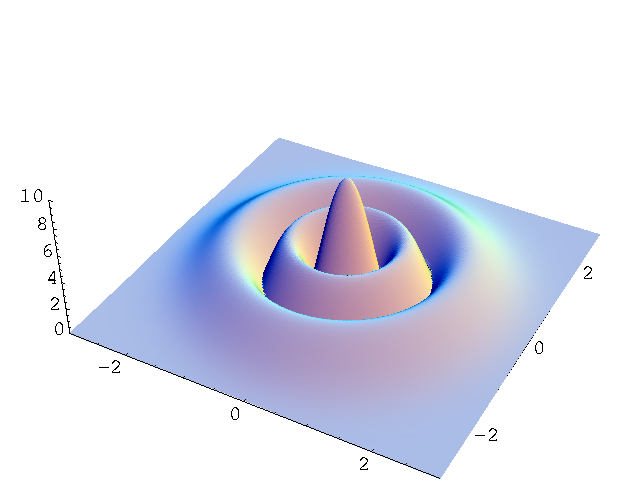
\includegraphics{GMS33.eps}
       \end{center}}
 \item \parbox[t]{130mm}{$B2sE>BP>N$G$J$$%=%j%H%s2r(BI\\
       \begin{center}
	$\begin{pmatrix}
	  0 & 0 & 1 & \cdots \\
	  0 & 0 & 0 & \cdots \\
	  1 & 0 & 0 & \cdots \\
	  \vdots & \vdots & \vdots & \ddots
	 \end{pmatrix}=$\\
	 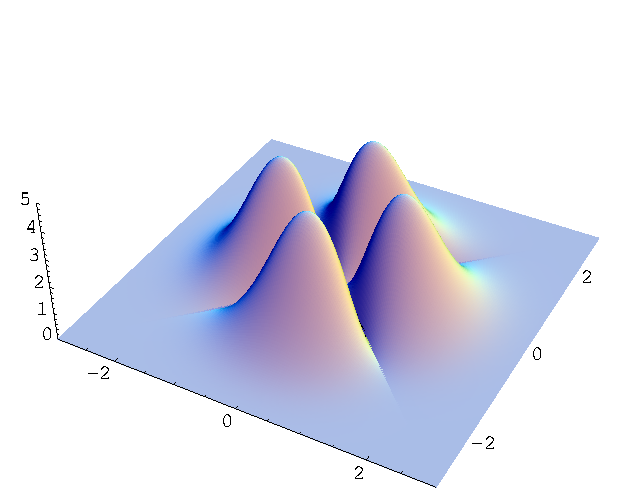
\includegraphics{GMS20.eps}
       \end{center}}
 \item \parbox[t]{130mm}{$B2sE>BP>N$G$J$$%=%j%H%s2r(BII\\
       \begin{center}
	$\begin{pmatrix}
	  0 & 0 & 0 & 0 & \cdots \\
	  0 & 0 & 0 & 0 & \cdots \\
	  0 & 0 & 0 & i & \cdots \\
	  0 & 0 & -i & 0 & \cdots \\
	  \vdots & \vdots & \vdots & \vdots &\ddots
	 \end{pmatrix}=$\\
	 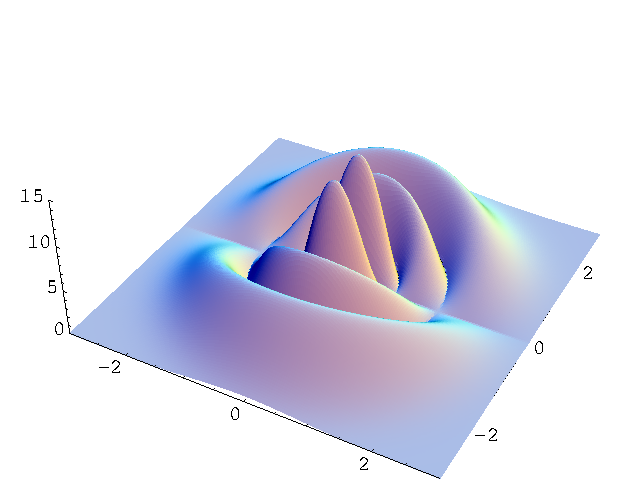
\includegraphics{GMS23I.eps}
       \end{center}}
\end{enumerate}


\subsubsection{$B9b<!85$X$N3HD%(B}

$B$3$l$^$G$O(B2$B<!85%f!<%/%j%C%I6u4V$N>l9g$r9M$($F$-$?$,!"$=$l$r(B$d+1$$B<!85(B
($+1$$B$O;~4V(B)$B$N>l9g$K3HD%$9$k!#$?$@$7;~4VJ}8~$OHs2D49@-$K4^$^$l$J$$$H$9$k!#(B
$B>l$NM}O@$G;~4VJ}8~$KHs2D49@-$rF~$l$?>l9g!"$=$N3HD%$O4JC1$G$"$k!#(B

$B$^$:!"(B$\theta^{\mu\nu}$$B$OH?BP>N9TNs$G$"$k$,!"E,Ev$J:BI8$ND>8rJQ49$K$h$C$F(B
\begin{equation}
 \theta^{\mu\nu}=
 \begin{pmatrix}
  \AntiSymBlock{\theta_1}& \zero & \cdots & \zero \\
  \zero & \AntiSymBlock{\theta_2}& \ddots & \vdots \\ 
  \vdots & \ddots & \ddots & \zero \\
  \zero & \cdots & \zero & \AntiSymBlock{\theta_{[d/2]}}\\
 \end{pmatrix}
\end{equation}
$B$H$J$k$h$&$K$9$k$3$H$,$G$-$k!#$9$k$H(B2$B<!85$N>l9g$K5"Ce$5$;$k$3$H$,$G$-$k!#(B
$B$3$&$7$FF@$i$l$?%=%j%H%s2r$O!"$?$@$N%=%j%H%s2r$+<+L@$J2r(B
($\phi(x)=\lambda_i$)$B$N@Q$K$J$C$F$$$k!#(B

\subsubsection{$B2r$N0BDj@-(B}

$B%=%j%H%s2r$rF@$k$3$H$O$G$-$?$,!"$3$l$i$N%=%j%H%s$,0BDj$J$b$N$H$7$FB8:_$7$F(B
$B$$$k$+$I$&$+$O<+L@$G$O$J$$!#$=$l$r3NG'$9$k!#(B

$B:#9M$($F$$$kM}O@$O!"(B(\ref{u-infinity-sym})$B$G<($7$?$h$&$J(B$U(\infty)$$B$NBP>N(B
$B@-$r$b$C$F$$$k$N$G$=$l$rMQ$$$F!"%=%j%H%s2r$r%*%Z%l!<%?$N8@MU$G(B$\ket{n}$$B$N(B
$B4pDl$K$D$$$FBP3Q$K;}$C$F$$$/$3$H$,$G$-$k!#$=$N$H$-$N2r$O!"(B
\begin{equation}
 \label{radial-solution}
 \begin{pmatrix}
  a_1 & 0 & \cdots & \cdots & \cdots & \cdots & 0 \\
  0 & a_2 & \ddots & \ddots & \ddots & \ddots & \vdots \\
  \vdots & \ddots & \ddots &\ddots &\ddots & \ddots & \vdots \\
  \vdots & \ddots & \ddots & a_n & \ddots & \ddots & \vdots \\
  \vdots & \ddots & \ddots &\ddots & 0 &  \ddots &\vdots \\
  \vdots & \ddots & \ddots &\ddots &\ddots & \ddots & \vdots \\
  0 & \cdots & \cdots & \cdots & \cdots & \cdots & 0 \\
 \end{pmatrix}
\end{equation}
$B$N$h$&$J7A$K$J$C$F$$$k!#C"$7!"(B$a_n$$B$O@h$K=R$Y$?$h$&$K!"%]%F%s%7%c%k(B$V$$B$NDd(B
$BN1E@(B$\lambda_i$$B$KCM$r$H$k!#$3$N2r$N%(%M%k%.!<$O(B
\begin{eqnarray}
 E &=& {2\pi\theta\over g^2}\Tr V(\phi) \nonumber \\
   &=& {2\pi\theta\over g^2}\sum^\infty_{n=0}V(a_n)
\end{eqnarray}
$B$H$J$k!#$7$?$,$C$F!"(B$a_n$$B$,%]%F%s%7%c%k(B$V$$B$N6K>.CM$G$"$l$P!"@]F0O@E*$K$O0B(B
$BDj$G$"$k$3$H$,J,$+$k!#(B

$B99$K!"(B$\theta\rightarrow\infty$$B$N6K8B$G$O!">l$N%(%M%k%.!<$,(B$\theta$$B$KHfNc(B
$B$7$F$$$k$N$G!"%]%F%s%7%c%k$NB>$N6K>.CM$dIi$NL58BBg$X$N%H%s%M%k$OM^@)$5$l$k(B
$B$N$GHs@]F0O@E*$K$b0BDj$G$"$k!#(B

\subsubsection{$\theta$$B$,M-8B$N;~$N(BGMS$B%=%j%H%s(B}

GMS$B%=%j%H%s$OHs2D49>l$NM}O@FCM-$NBP>]$G$"$k!#$7$?$,$C$F!"(B$\theta$$B$rM-8B$K(B
$B$7$F$=$N@dBPCM$r(B$0$$B$K$9$k$H(BGMS$B%=%j%H%s$OL5$/$J$C$F$7$^$&$3$H$,M=A[$5$l$k!#(B
$B$=$l$O;v<B$G$"$j!"<B:]$K$O(B$\theta$$B$N8:>/$KH<$J$C$F(BGMS$B%=%j%H%s2r$,L5$/$J$C(B
$B$F$7$^$&$3$H$,J,$+$k!#(B\cite{NCSolFinTheta}

$\theta$$B$,M-8B$N;~$O!"1?F09`$r9M$($J$/$F$O$J$i$J$$!#$^$:!"HyJ,$O:BI8$N%j(B
$B%9%1!<%k$N8e!"(B
\begin{equation}
 \left\{
  \begin{array}{l}
   \partial_x\rightarrow i[\yh,\cdot]
    ={1\over\sqrt{2}}[\anih -\crea,\cdot]\\
   \partial_y\rightarrow -i[\xh,\cdot]
    =-i{1\over\sqrt{2}}[\anih +\crea ,\cdot]\\
  \end{array}
 \right.
\end{equation}
$B$H=q$/$3$H$,$G$-$k!#$9$k$H!"(B
\begin{equation}
 \int dxdy\, \1half\left(\partial_x\phi^2+\partial_y\phi^2\right)
  =\pi \Tr ([\crea,\hat{\phi}][\anih,\hat{\phi}])
\end{equation}
$B$H$3$m$G!"$3$N1?F09`$O(B$\crea$$B$d(B$\anih$$B$r4^$s$G$$$k$N$G!"@h$K=R$Y$?(B
$U(\infty)$$B$NBP>N@-$r2u$7$F$7$^$&!#$h$C$F!"2sE>BP>N$J2r$K>o$K;}$C$F$$$1$k(B
$B$H$O8B$i$J$$$,!"$3$3$G$O2sE>BP>N$J(B\ref{GMSradial-solution}$B$N$h$&$J2r$N$_$r(B
$B9M$($k!#$9$k$H!"%*%Z%l!<%?$N8@MU$G=q$+$l$?%O%_%k%H%K%"%s$O!"(B
\begin{equation}
 \Ham =\sum_{n=0}^\infty {1\over 4}
  [(2n+1)a_n^2-2(n+1)a_na_{n+1}]+\theta V(a_n)
\end{equation}
$B$H$J$k!#8EE5E*$J2r$O(B
\begin{equation}
 {\partial\Ham\over\partial a_n}=0
\end{equation}
$B$K$h$C$FF@$k$3$H$,$G$-$k!#$3$l$O!"(B
\begin{equation}
 \left\{
  \begin{array}{ll}
   (n+1)a_n-(2n+1)+na_{n-1}=2\theta V'(a_n)\hspace{5mm}& (n\geq1) \\
   a_1-a_0=2\theta V'(a_0)\hspace{5mm}& (n=0\hbox{$B$KBP1~(B}) \\
  \end{array}
\right.
\end{equation}
$B$H$$$&L58B8D$N:9J,J}Dx<0$K$J$k!#3F<0$r(B$N$$B$^$GB-$79g$o$;$k$H!"(B$\theta$$BM-(B
$B8B$N;~$N2sE>BP>N$J%=%j%H%s2r$N%*%Z%l!<%?!<$K$h$kI=8=$NBP3Q@.J,(B
$a_n$$B$NK~$?$9$Y$-<0$N:G=*7A$O!"(B
\begin{equation}
 \label{finite-theta-equation}
 a_{N+1}-a_N={2\theta\over N+1}\sum^N_{n=0} V'(a_n)
\end{equation}
$B$H$$$&<0$K$J$k!#99$K!"%(%M%k%.!<$,M-8B$G$"$k$3$H$rMW5a$9$k$H!"(B
\begin{equation}
 \label{finite-theta-convergence-condition}
 \left\{
 \begin{array}{l}
  a_n\rightarrow0\quad(n\rightarrow\infty)\\
  \sum\limits_{n=0}^\infty V'(a_n)<\infty \\
 \end{array}\right.
\end{equation}
$B$H$$$&I,MW>r7o$,$G$k!#(B

$B$3$3$G!"(B$\theta$$B$r(B$0$$B$K6a$E$1$k$3$H$r9M$($F$_$k!#(BGMS$B%=%j%H%s$O;~6u$NHs2D(B
$B49@-$,$"$C$F;O$a$FB8:_$9$k$b$N$G$"$k$3$H$+$i!"(B$\theta\rightarrow 0$$B$G(BGMS 
$B%=%j%H%s$O>C$($F$7$^$&$O$:$G$"$k!#@_Dj$H$7$F!"(B$T=0$$B$r??$N??6u$K$H$C$F9M(B
$B$($k!#(B(\ref{finite-theta-equation})$B$r8+$k$H!"(B$\theta$$B$O(B$a_n$$B$,F0$/I}$r5,(B
$BDj$7$F$$$k$3$H$,J,$+$k!#(B$\theta$$B$,==J,>.$5$$;~$O!"(B$a_n$ $B$NJQ2=$,Hs>o$K>.(B
$B$5$$$N$G<0(B(\ref{finite-theta-equation})$B$N1&JU$O@QJ,$H$7$FNI$$6a;w$K$J$k!#(B
$BB($A!"(B
\begin{align}
 a_{n+1}-a_n\simeq 2\theta\int^{a_n}_{a_0}da\, V'(x)&=2\theta(V(a_n)-V(a_0))
  \nonumber\\
 &\xrightarrow{n\rightarrow\infty}-2\theta V(a_0)
\end{align}
$B$H$J$k!#$h$C$F!"(B(\ref{finite-theta-convergence-condition})$B$rK~$?$90Y$K$O!"(B
$V(a_0)=0$$BB($A(B$a_0=0$$B$G$J$/$F$O$J$i$J$$!#$7$+$7!"$3$N=i4|>r7o$G:9J,(B
$BJ}Dx<0(B(\ref{finite-theta-equation})$B$r2r$/$H!"<+L@$J2r$7$+M?$($J$$!#$h$C(B
$B$F!"(B$\theta$$B$,==J,>.$5$/$F!":9J,J}Dx<0(B(\ref{finite-theta-equation})$B$N1&(B
$BJU$NOB$r@QJ,$H$7$F8+$k$3$H$,$G$-$k$H$-$O!"<+L@$J2r$7$+L5$$$3$H$,J,$+$C$?!#(B

$B$3$l0J>e$N5DO@$r?J$a$k$?$a$K$O6qBNE*$K%]%F%s%7%c%k$N7A$rM?$($F?tCME*$J7W(B
$B;;$r9T$J$o$J$/$F$J$J$i$J$$!#%]%F%s%7%c%k$N7A$rM?$($F?tCME*$K2r@O$7$?5DO@(B
$B$O(B\cite{NCSolFinTheta}$B$G$J$5$l$F$$$k!#(B

\subsubsection{$\theta$$B$,M-8B$G%2!<%8>l$,$"$k;~(B}

$B>e$G8+$?$h$&$K!"%9%+%i!<>l$@$1$N;~$K$O(B$\theta$$BM-8B$GHs<+L@$J2r$r9=@.$7$h(B
$B$&$H$7$F$b7k6I:9J,J}Dx<0$K5"Ce$9$k$N$_$@$,!"%2!<%8>l$,B8:_$9$k;~$K$O1?F0(B
$B9`$,F~$C$F$$$F$b(B$U(\infty)$$B$NBP>N@-$,2sI|$9$k(B\footnote{$U( \infty)$$B$NL5(B
$B8B>.JQ49(B$1+\lambda$($\lambda$:Hermite)$B$KBP$7$F(B$A_\mu \rightarrow A+
\partial_\mu\lambda$$B$H$9$l$P$h$$!#(B}$B$N$G!"2r@OE*$J87L)2r$r9=@.$9$k$3$H$,(B
$B$G$-$k!#(B

$B$^$:!"6qBNE*$J2r$r5a$a$kA0$K%*%Z%l!<%?!<7A<0$G(B$U(\infty)$$BBP>N@-$,B8:_$9(B
$B$k;~$K%=%j%H%s2r$r9=@.$9$k0lHLE*$JJ}K!(B\cite{ExactNCSol}$B$K$D$$$F@bL@$9$k!#(B

$B:#!"(BHilbert$B6u4V$K:nMQ$9$k1i;;;R(B$U$$B$r9M$($k$H!"(B$U$$B$N:nMQ$O(B
\begin{equation}
 \begin{split}
  \ket{\psi}\rightarrow U\ket{\psi} \\
  \bra{\psi}\rightarrow \bra{\psi}\Ud \\
  \OpO\rightarrow U\OpO\Ud
 \end{split}
\end{equation}
$B$H$J$k!#$b$7(B$U$$B$,(Bisometry$B$G$"$kB($A(B
\begin{equation}
 \label{isometry}
  U\Ud=1
\end{equation}
$B$rK~$?$7!"$7$+$7$J$,$i%f%K%?%j$G$O$J$i$P!"JQ49(B$U$$B$K$h$C$F1?F0J}Dx<0$N2r(B
$B$OJL$N2r$X$HJQ49$5$l$k!#(B($U$$B$,%f%K%?%j$J$i$PK\<AE*$KF1$82r$X$HJQ49$5$l$k!#(B)
$B2?8N$J$i$P!"J*M}E*<+M3EY$rI=$o$91i;;;REy$r4^$`0lHL$N1i;;;R$KBP$7$F(B
\begin{equation}
 \frac{\delta S}{\delta \OpO}\rightarrow
  U\frac{\delta S}{\delta \OpO}\Ud
\end{equation}
$B$H$J$k$+$i!"7PO)@QJ,$N6KCM$rM?$($k$h$&$JG[0L$rJL$N7PO)@QJ,$N6KCM$rM?$($k(B
$B$h$&$JG[0L$KJQ49$9$k$+$i$G$"$k!#$3$N$h$&$JJQ49(B$U$$B$r(Bsolution generating
transformation $B$H$$$&!#(B

$B$3$3$G!"(BHilbert$B6u4V$H$7$F(B1$B8D$ND4OB?6F0;R$,@.$9(BFock$B6u4V$r9M$($k!#(Bshift
operator$S$$B!"(B
\begin{equation}
 \label{shift-operator}
 S\equiv\sum^\infty_{k=o}\ket{k+1}\bra{k}
\end{equation}
$B$O!"(B
\begin{equation}
 \Sd^nS^n=1,\quad S^n\Sd^n=1-P_n
\end{equation}
$B$H$$$&4X78$rK~$?$9!#C"$7!"(B
\begin{equation}
 P_n=\sum^{n-1}_{k=0}\ket{k}\bra{k}
\end{equation}
$B$G$"$k!#(B$S^n$$B$O<0(B(\ref{isometry})$B$rK~$?$9$N$G(Bsolution generation
transformation$B$G$"$k!#:#(B$S^n\Sd^n$$B$O(BHilbert$B6u4V$N(B$\ket{0}\sim\ket{n-1}$ 
$B$K1w$$$F$N$_%f%K%?%jJQ49$G$J$$!#(B$\ket{n}$$B$OH>7B(B$\sqrt{n\theta}$$B$NNN0h$K(B
$BBP1~$7$F$$$?$+$i!"2r@8@.JQ49(B$S^n$$B$K$h$C$F!"H>7B(B$\sqrt{n\theta}$$B$NHs2D49(B
$B%=%j%H%s$r:n$k$3$H$,$G$-$k$H9M$($k$3$H$,$G$-$k!#(B

$B6qBNE*$J7W;;$K0\$k$H!":#9M$($k:nMQ$O(B
\begin{equation}
 \int dxdy\, \left(\1half(F_{xy})^2
	      +\1half D^\mu\phi D_\mu\phi -V(\phi)\right)
\end{equation}
$B$G$"$k!#$3$l$r:BI8$N%j%9%1!<%k$N8e$K!"%*%Z%l!<%?!<$N8@MU$K=q$-D>$9!#JX59(B
$B$N0Y!"%2!<%8>l$O<!$N$h$&$KI=5-$9$k$3$H$K$9$k!#(B
\begin{equation}
 A\equiv A_z=-\frac{i}{\sqrt{2}}(A_x-iA_y),\quad
  \Ab\equiv A_{\zb}=-\frac{i}{\sqrt{2}}(A_x+iA_y)
\end{equation}
$B<!$K6&JQHyJ,$r%*%Z%l!<%?!<$N8@MU$G=q$/$3$H$r9M$($k(B
\begin{equation}
 \creC\equiv \anih+i\theta^{\1half}A,\quad
  \aniC\equiv \crea-i\theta^{\1half}\Ab
\end{equation}
$B$H$9$k$H!"(B
\begin{eqnarray}
 \frac{1}{\sqrt{2}}[D_x-iD_y,\phi]=-[\aniC,\phi]
 \frac{1}{\sqrt{2}}[D_x+iD_y,\phi]=[\creC,\phi]
\end{eqnarray}
$B$3$N6&JQHyJ,$r;H$C$F(Bfield strength$B$O%*%Z%l!<%?!<$N8@MU$G<!$N$h$&$K=q$1$k!#(B
\begin{equation}
 F\equiv -F_{xy}=-i[\crea,\Ab]-i[\anih,A]+\theta^{\1half}[A,\Ab]
  =\theta^{-\1half}([\aniC,\creC]+1)
\end{equation}
$B7k6I!"%*%Z%l!<%?!<7A<0$G=q$+$l$?%O%_%k%H%K%"%s$O(B
\begin{equation}
 \Ham=2\pi\Tr\left(\1half([\aniC,\creC]+1)^2
		 +[\aniC,\phi][\creC,\phi]
		 +\theta V(\phi)\right)
\end{equation}
$B$H$J$k!#$3$N7O$N<+L@$J2r$O(B$\phi_*$$B$r(B$V(\phi)$$B$N6K>.CM$rM?$($k(B$\phi$$B$NCM(B
$B$H$7!"99$K(B$V(\phi_*)=0$$B$9$l$P!"(B
\begin{equation}
 \begin{split}
  \phi&=\phi_*\\
  A&=0\Rightarrow \creC=\anih,\,\aniC=\crea
 \end{split}
\end{equation}
$B$G$"$k!#$3$l$r@h$N(Bsolution generating transformation$B$K$h$C$FJL$N2r$K<L$9$H!"(B
\begin{equation}
 \begin{split}
  \phi&=\phi_*(1-P_n) \\
  \creC&=S^n\anih\Sd^n,\,\aniC=S^n\crea\Sd^n
 \end{split}
\end{equation}
$B$H$J$k!#$3$l$OHs<+L@$J2r$G$"$k!#$3$N;~(Bfield strength$B$O!"(B
\begin{equation}
 F=\theta^{-\1half}([\creC,\aniC]-1)=\theta^{-\1half}(S^n\Sd^n-1)
  =\theta^{-\1half}P_n
\end{equation}
$B$G$"$j!"(B$[\creC,S^n\Sd^n]=0$$B$H$J$k$+$i!"$3$N2r$N;}$D%(%M%k%.!<$O(B
\begin{equation}
 E=2\pi n\left(\frac{1}{2\theta}+\theta V(0)\right)
\end{equation}
$B$H$J$k!#(B

 \input{d-brane}
 %#!platex master.tex
\subsection{TypeIIB$BM}O@$G$N(BToeplitz$BBe?t$H;X?tDjM}(B}

\subsubsection{$B\rightarrow\infty$$B6K8B$G$NBe?t$NJ,2r(B}

$B89M}O@$KI=$o$l$k(BOPE$BBe?t$O$$$/$D$+$NItJ,Be?t$r;}$C$F$$$k!#$=$NCf$G$b!"(B
$\AlgA_0$$B$r2D49$JJ}8~$N89$N=E?4:BI8$K0M$i$J$$ItJ,Be?t$9$J$o$A!"(B$b,c,\der
X, \der^2X, \ldots$$B$H$=$N@Q$+$i$J$kBe?t$H$9$k!#$3$NBe?t(B$\AlgA_0$$B$,Be?t$H(B
$B$7$FJD$8$F$$$k$H$O1?F0NL$NJ]B8$+$iD>46E*$KM}2r$G$-$k!#(B\footnote{$B$3$3$G$O(B
$g_{ij}$$B$,BP3Q7A$G$"$k$3$H$r2>Dj$7$F$$$k!#(B}$B$^$?!"(B$\AlgA_1$$B$r(B$p$$BHs2D49J}(B
$B8~$N1?F0NL$H$7$F!"(B$\E^{iX\cdot p}$$B$N7A$N85$+$i$J$k=89g$H$9$k!#$3$N=89g$O(B
$BIaDL$O(BOPE$BBe?t$H$7$FJD$8$J$$$,(B$B\rightarrow\infty$ $B$N6K8B$r$H$k$3$H$G$3$N(B
$B=89g$r(BOPE$BBe?t$H$7$FJD$8$5$;$k$3$H$,$G$-$k!#99$K$O!"(BOPE$B$NBe?tA4BN(B$\AlgA$
$B$O(B$\AlgA=\AlgA_0\otimes \AlgA_1$$B$HJ,2r$9$k!#(B

$B$^$::G=i$K$3$NJ,2r$r3N$+$a$k!#(B$B$$B>l$NB8:_$9$k;~$N(Bworld sheet$B$N6-3&>e$N%P!<(B
$B%F%C%/%91i;;;R(B$X^i$$B$N(BOPE$BB($A!"(Bpropagator$B$O<0(B(\ref{bdry-propag})$B$G4{$K5a(B
$B$a$?$h$&$K!"(B
\begin{equation}
 X^i(\tau)X^j(\tau')
  \sim -\ap\left(\frac{1}{g+2\pi\ap B}\right)_{\mbox{$BBP>N(B}}\ln(\tau-\tau')^2
  -i\pi\ap\left(\frac{1}{g+2\pi\ap B}\right)_{\mbox{$BH?BP>N(B}}
  \epsilon(\tau-\tau')
\end{equation}
$B$N$h$&$J7A$K$J$k!#$3$3$G!"(B$B\rightarrow\infty$$B$N6K8B$r<h$j99$K(B$X$$B$N%j%9(B
$B%1!<%k$r9T$J$&!#(B$B\rightarrow tB$$B$HCV$-49$($F!"(B$X^i\rightarrow X^i
\diagup\sqrt{t}$$B$HCV$-49$($F!"(B$t\rightarrow\infty$$B$N6K8B$r<h$k$H!"@h$K5a(B
$B$a$?(Bpropagator$B$O(B
\begin{equation}
 X^i(\tau)X^j(\tau')\sim\left\{\begin{array}{ll}
			\ihalf\theta^{ij}\epsilon(\tau-\tau')
			 &\quad\mbox{($i,j$$BHs2D49J}8~(B)}\\
			\frac{1}{t}g^{ij}
			 &\quad\mbox{($i,j$$B2D49J}8~(B)}\\
			\frac{(\theta^2)^{ij}}{t(2\pi)^2\ap}
			 &\quad\mbox{($B$=$l0J30(B)}
			\end{array}\right.
\end{equation}
$B$H$J$k!#$5$i$K$3$N6K8B$G$N=E?4:BI8$r4^$^$J$$Be?t(B$\AlgA_0$$B$r9M$($k$H!"$3(B
$B$NBe?t$N85$N$&$A!"Hs2D49J}8~$N(B$X^i$$B$r4^$`85$O!"%j%9%1!<%k$N1F6A$r<u$1$F(B
$B!"3F(B$\der^nX^i$$B$K$D$$$F(B$\sqrt{t}$$BG\$5$l$k!#(B

$B$^$:$3$N6K8B$G!"(B$\AlgA_0$$B$H(B$\AlgA_1$$B$,8r49$9$k$3$H$r3N$+$a$k!#(B$\AlgA_0$
$B$N85$H(B$\AlgA_1$$B$N85$N(BOPE$B$G8r49$9$k$+$I$&$+2x$7$$$N$O!"0J2<$N(BOPE$B$G$"$k!#(B
\begin{equation}
 \sqrt{t}\der^nX^i(\tau)\E^{iq\cdot X}\sim\frac{1}{\sqrt{t}}
  (\tau-\tau')^{-n}\E^{iqX}
\end{equation}
$B1&JU$r8+$k$H!"(B$t\rightarrow\infty$$B$N6K8B$G$3$N(BOPE$B$O>C$($F$7$^$&!#(B

$B<!$K(B$\AlgA_1$$B$,Be?t$H$7$FJD$8$F$$$k$3$H$r3N$+$a$k!#(B
\begin{equation}
 \E^{ipX}(\tau)\E^{iq\cdot X}(\tau')\sim\E^{-\ihalf p^i\theta_{ij}q^j}
  \E^{(p+q)\cdot X}(\tau')(1+i(\tau-\tau')p\cdot X)
\end{equation}
$B$G$"$k$,!"1&JU$N(B$p\cdot X$$B$N9`$O(B$X^i$$B$,Hs2D49J}8~$G$"$k$K$b94$i$:(B
$\sqrt{t}$$B$N(Bfactor$B$,$+$+$C$F$$$J$$$N$GL5;k$9$k$3$H$,$G$-$k!#(B

$B0J>e$G!"(B$B\rightarrow\infty$$B$N6K8B$G(B$\AlgA$$B$,(B$\AlgA_0\otimes\AlgA_1$$B$KJ,(B
$B2r$9$k$3$H$,8@$($?!#(B$\AlgA_1$$B$OHs2D49$JJ}8~$N1?F0NL$N(BFourier$B@.J,$N$_$+$i(B
$B9=@.$5$l$F$$$k$N$G!"Hs2D49J}8~$N4X?t4D$G$"$k$H2r<a$9$k$3$H$,$G$-$k!#(B

\subsubsection{Toeplitz$B:nMQAG$H;X?tDjM}(B}

$B$$$^!"(BD9-D\={9}$B7O$r9M$($k!#$3$N;~(Bstring field$B$O(B$2\times 2$$B$N(BChan-Paton$B9T(B
$BNs$G5-=R$5$l$k$,!"(B9-\={9}string$B$O5U8~$-$N(BGSO projection$B$,$+$+$k$N$G!"(B
string field$B$O<!$N$h$&$J7A$r$7$F$$$k!#(B
\begin{equation}
 A=\begin{pmatrix}
    B&C\\ C^* &B'
   \end{pmatrix}
\end{equation}
$B$3$3$G(B

D9-D\={9}$B7O$+$i!"(Bclosed string vacuum$B$X$NA+0\$r5-=R$9$k$h$&$J(BString
field theory$B$N1?F0J}Dx<0(B
\begin{equation}
 \label{sft-eom}
 Q(A)+A*A=0
\end{equation}
$B$N8EE52r$,B8:_$9$k$H$$$&;v$,!"(BString field theory$B$G?.$8$i$l$F$$$k!#$3$N(B
$B$h$&$J2r$r(B
\begin{equation}
 A_0=\begin{pmatrix}
      \alpha & \beta \\ \beta^* & \gamma
     \end{pmatrix}
\end{equation}
$B$H=q$/$9$k$3$H$K$9$k!#(B

$B\rightarrow\infty$$B$N6K8B$G$O@hDx=R$Y$?$h$&$K!"%P!<%F%C%/%9$NBe?t(B
$\AlgA$$B$,(B$\AlgA_0\otimes\AlgA_1$$B$HJ,2r$9$k$+$i!"(B$\Tb$$B$r(B$\AlgA_0$$B$N85(B
$B$H$7$F?7$?$J2r$r<!$N$h$&$K$7$F$D$/$k$3$H$,$G$-$k!#(B
\begin{equation}
 \begin{pmatrix}
  \alpha\otimes\Tb T&\beta\otimes \Tb\\
  \beta^\dagger\otimes T & \gamma\otimes T\Tb
 \end{pmatrix}
\end{equation}
$B$H$9$l$P!"$3$N2r$,1?F0J}Dx<0(B(\ref{sft-eom})$B$rK~$?$90Y$K$O(B$T$$B$,(B
\begin{equation}
 \label{ttt-t}
 T\Tb T=T,\quad\Tb T\Tb=\Tb
\end{equation}
$B$rK~$?$5$J$1$l$P$J$i$J$$!#$3$N<+L@$J2r$H$7$F(B$T$$B$,%f%K%?%j$G$"$k$H$-$K$O(B
$T$$B$N8GM-CM$r(B$\E^{i\varphi}$$B$H$9$l$P(B
\begin{equation}
 \begin{pmatrix}
  \alpha & \beta\E^{i\varphi} \\ \beta^\dagger\E^{-i\varphi} & \gamma
 \end{pmatrix}
\end{equation}
$B$J$k2r$rF@$k$,!"$3$l$O(BString field theory$B$N%?%-%*%s6E=L$N7O$G85$+$i$"$k(B
$BBP>N@-(B$C\rightarrow\E^{i\varphi}$$B$G2r(B$A_0$$B$H85$+$i7k$P$l$F$$$k2r$G$"$k!#(B

$BHs<+L@$J$N$O!"(B$T$$B$,%f%K%?%j$G$O$J$$$,<0(B(\ref{ttt-t})$B$rK~$?$9;~$G$"$k!#$=(B
$B$N4JC1$JNc$H$7$FHs2D49J}8~$,(B2$B<!85$G$"$k>l9g$r9M$($k!#$9$J$o$A!"(B
\begin{equation}
 [x,y]=-i\theta\quad(\theta>0)
\end{equation}
$B$3$N;~!"0JA0$HF1$8<jB3$-$G@8@.(B\ten $B>CLG1i;;;R$r:n$k$3$H$,$G$-$k!#B($A!"(B
\begin{equation}
 \anih=\frac{x-iy}{\sqrt{2\theta}},\quad\crea=\frac{x+iy}{2\theta}
 ,\quad [\anih,\crea]=1
\end{equation}
$B$9$k$H!"0J2<$N$h$&$KDj5A$7$?(B$T$$B$O<0(B(\ref{ttt-t})$B$rK~$?$9!#(B
\begin{align}
 T&=\frac{1}{\sqrt{\crea\anih+1}}\anih\\
 \Tb&=\crea\frac{1}{\sqrt{\crea\anih+1}}
\end{align}

$B$3$3$G!"(BHilbert$B6u4V(B$\Hil$$B$N>e$N1i;;;R$K$O(BFredholm$B1i;;;R$H$$$&35G0$,$"$j!"(B
Fredholm$B1i;;;R$K$O;X?t$,Dj5A$5$l$F$$$k!#(B
\begin{Def}[Fredholm$B1i;;;R(B]
 Hilbert$B6u4V$N>e$NM-3&$J1i;;;R(B$T\in\AlgB(\Hil)$$B$,(BFredholm$B1i;;;R$G$"$k$H(B
 $B$O!"(B$\Img T$$B$,JD=89g$K$J$C$F$$$F(B$\Ker T,\Ker T^*$$B$,6&$KM-8B<!85$G$"$k$3(B
 $B$H$r$$$&!#(B
\end{Def}
$B$3$N;~(B$T$$B$K$D$$$F!";X?t$O(B
\begin{equation}
 \Ind(T)=\Dim(\Ker T)-\Dim(\Ker T^*)
\end{equation}
$B$K$h$C$FDj5A$5$l$F$$$k!#(B

$B:#(B$T$$B$O(BToeplitz$B1i;;;R$K$J$C$F$$$k!#$3$3$G(BToeplitz$B1i;;;R$H$O0J2<$GDj5A$5(B
$B$l$k$h$&$JBe?t$N85$G$"$k!#(B
\begin{Def}[Toeplitz$BBe?t(B]
 $B>hK!C10L85$r$b$D(B$\Cst$$B4D$NItJ,4D$G(B$SS^*=1,S^*S\neq 1$$B$rK~$?$9(B$S$
 $B$+$i@8@.$5$l$k(B$\Cst$$BItJ,4D$r(BToeplitz$BBe?t$H$$$&!#(B
\end{Def}
$B$3$NNc$H$7$F$O!"(BGMS$B%=%j%H%s(B(\ref{GMSsoliton}$B>.@a(B)$B$N:G8e$NJ}$GDj5A$7$?(B
shift operator $S$ (\ref{shift-operator})$B$G@8@.$5$l$k(B$\Cst$$B4D$,$"$k!#$3(B
$B$l$O!"(BHilbert$B6u4V>e$NM-3&:nMQAG$N@.$9(B$\Cst$$B4D$N(BToeplitz$BBe?t$K$J$C$F$$$k!#(B
$B:#$NNc$G(B

$B:#!"5a$a$?(B$T$$B$K$D$$$F;X?t$r7W;;$9$k$H(B
\begin{equation}
 \Ind(T)=1
\end{equation}
$B$G$"$k!#$=$N0lJ}$GHs2D496u4V>e$N4X?t(B$T$$B$r(B$x,y$$B$GI=$o$9!"B($A5U(BWeyl$B<LA|$r(B
$B$9$k$H!"(B
\begin{equation}
 f(r)(x-iy)
\end{equation}
$B$N7A$K$J$C$F$$$k!#$3$l$O!"86E@6aK5$G(B$U(1)$$B$K$D$$$F4,$-IU$-?t(B$-1$$B$NG[0L$K(B
$B$J$C$F$$$k!#$h$C$F!"0lHL$K%?%-%*%s>l$N4,$-IU$-?t$O(B$-\Ind(T)$$B$GM?$($i$l$k!#(B
$B$3$l$O!"(BAtiyah-Singer$B$N;X?tDjM}$N0lNc$K$J$C$F$$$k!#(B

\subsubsection{$BM><!85$,(B$2n$$B$N;~$N;X?tDjM}(B}
$B:#!"6u4V(B$X$$B$NM><!85(B$2n$ $B$NItJ,6u4V(B$Y$$B$r9M$($k!#:#EY$O!"(B10$B<!85$N;~6u$K(B
$2^p$$BKg$N(BD9-brane$B$H(BD\={9}-brane$B$NBP$,$"$k$3$H$r9M$($k!"$3$N7O$,;}$AF@$k(B
D-brane$B%A%c!<%8$r9M$($k!#$3$N;~$=$NM><!85$,Hs2D49(B$\Real^{2n}$ $B$K$J$C$F$$(B
$B$k$H$9$k!#$=$NHs2D49@-$O0lHL$K(B
\begin{equation}
 [x^{2i-1},x^{2i}]=-i\theta_i\quad(\theta_i>0)
\end{equation}
$B$H=q$/$3$H$,$G$-$k!#(B

$B99$K!"(BClifford$BBe?t$N(B$2^n$$B<!85$NI=8=(B$\gamma_i$$B!"(B
\begin{equation}
 \gamma_i=\begin{pmatrix}
	   0 &\Gamma_i\\
	   \bar{\Gamma}_i &0
	  \end{pmatrix}
\end{equation}
$B$K$h$C$FHs2D496u4V>e$N%?%-%*%s>l!"(B
\begin{equation}
 T\equiv f(r)\Gamma_ix^i:\Hil\otimes\Spi^-\rightarrow\Hil\otimes\Spi^+
\end{equation}
$B$r9M$($k!#$3$3$G!"(B$\Hil$$B$O(B$p$$B8D$ND4OB?6F0;R$N@.$9(BFock$B6u4V$G$"$k!#$3$3$G!"(B
$N_i$$B$r(B$i$$BHVL\$ND4OB?6F0;R$N(Bnumber operator$B$H$7$F!"(B
\begin{align}
 \Gamma_ix^i\bar{\Gamma_j}x^j&=\frac{1}{4}\{\Gamma_i,\bar{\Gamma}_j\}
  \{x^i,x^j\}+\frac{1}{4}[\Gamma_i,\bar{\Gamma}_j][x^i,x^j]\nonumber\\
 &=\frac{1}{2}\delta^{ij}\{x_i,x_j\}+\sum_i\sigma^3_i\theta^i\nonumber\\
 &=\sum_i2\theta_i(N_i+\frac{1}{2})+\sum_i\sigma^3_i\theta^i\\
 \bar{\Gamma}_ix^j\Gamma_jx^j
 &=\sum_i2\theta_i(N_i+\frac{1}{2})+\sum_i\sigma^3_i\theta^i
\end{align}
$B$G$"$k$+$i!"(B$T$$B$r(B
\begin{equation}
 \label{T-gamma}
 T=\Gamma_ix^i\frac{1}{\sqrt{\Gamma_ix^i\bar{\Gamma}_jx^j}}
\end{equation}
$B$H$9$l$P!"$3$N(B$T$$B$O(B
\begin{equation}
 T\Tb T=T,\quad\Tb T\Tb=\Tb
\end{equation}
$B$rK~$?$7!"(B$\Spi^-$$B$N%9%T%s$,(B$(-\frac{1}{2},\ldots,-\frac{1}{2})$$B$G$"$k;~(B
$T$$B$O<!85(B1$B$N%+!<%M%k$r;}$D!#$h$C$F!"(B$T$$B$N;X?t$O(B
\begin{equation}
 \Ind(T)=-1
\end{equation}
$B$H7W;;$5$l$k!#(B

$B99$K!"$3$N;X?t$H4,$-IU$-?t$H$N4X78$r8+$k!#:#!"(B$Y$$B$NM><!85$G$"$k(B
$\Real^{2n}$$B$r9M$($F!"(B$z_i=x^{2i-1}+ix^{2i}$$B$H$7$?;~$N@5B'4X?t$+$i$J$k(B
Hilbert$B6u4V(B$\Hil$$B$r9M$($k!#$3$N(BHilbert$B6u4V$N4pDl$O(B$z^k\equiv
\prod_{i=0}^k(z_i)^k_i$$B$G$"$k!#99$K!"(B$\Real^{2n}$$B$NCf$N(B$2n-1$ $B<!85$N5eLL(B
$\Sigma^{2n-1}$$B$K$D$$$F!"$=$N>e$N@5B'4X?t$+$i:n$k(BHilbert$B6u4V(B
$\Hil_\Sigma$$B$r9M$($k!#$3$N5eLL>e$N(B2$B>h2D@QJ,$J4X?t(B$f\in L^2(\Sigma ;d
\Omega)$$B$+$i(B$\Hil_\Sigma$$B$X$NJQ49(B$P$$B$O<!$N$h$&$KM?$($i$l$k!#(B
\begin{equation}
 (Pf)(z)\equiv\int_\Sigma\frac{f(w)}{(1-z\cdot\bar{w})}d\Omega
\end{equation}
$B$3$N$h$&$K$7$FDj5A$5$l$k(BHilbert$B6u4V(B$\Hil_\Sigma$$B$r(BHardy$B6u4V$H$$$&!#$3$N(B
$\Hil_\Sigma$$B$ND>8r4pDl$O$d$O$j(B$z^k$$B$GM?$($i$l$k!#$?$@$7!"(B$\Hil_\Sigma$
$B$G$N%N%k%`$O(B
\begin{equation}
 (z^k,z^{k'})\equiv\delta_{k,k'}\frac{2\pi^p\prod_i(k_i)!}{
\Gamma(\sum_ik_i+p)}
\end{equation}
$B$H=q$/$3$H$,$G$-$k!#$3$NHs2D49(B$\Real^{2n}$$B$K4X$9$k(BHilbert$B6u4V$+$i(BHardy$B6u(B
$B4V$X$N@)8B<LA|$O(B1$BBP(B1$B$G>e$X$N<LA|$K$J$C$F$$$k$N$G!"(BT$B$N;X?t$O(BT$B$N(B
$\Hil_\Sigma$$B$X$N@)8B$N;X?t$HF1$8$K$J$k!#(B

$B$3$N(BHardy$B6u4V$K$D$$$F(BToeplitz$B:nMQAG$rDj5A$9$k$3$H$,$G$-$k!#B($A!"(B
$\Sigma$$B>e$N4X?t(B$f$$B$K$D$$$F!"(B$M_f:\Ham_\Sigma\rightarrow
L^2(\Sigma;d\Omega)$$B$O(BHardy$B6u4V>e$N1i;;;R$r(B$\Sigma$$B>e$N4X?t$KD>$7$F!"(B$f$ 
$B$r3]$1$k$H$$$&1i;;;R$H$9$l$P!"(B
\begin{equation}
 \Toep_f\equiv PM_f
\end{equation}
$B$H$$$&1i;;;R$rDj5A$9$k$3$H$,$G$-$k!#(B
\begin{align}
 \Toep_{z_i}z^k&=z^{k+e_i}\\
 \Toep_{\zb_i}z^k&=0\quad(k_i=0)\\
 &=2\pi\frac{k_i}{\sum_ik_i+p-1}z^{k-e_i}
\end{align}
$B$G$"$j!"$3$N(B$\Toep$$B$O(BToeplitz$B1i;;;R$K$J$C$F$$$k!#(B

$B:#!"(BHilbert$B6u4V$H$7$F(B$\Hil_\Sigma\otimes\Cplx^{2^N}$$B$r$H$l$P!"1i;;;R$r9T(B
$BNsCM$N1i;;;R$KMF0W$K3HD%$9$k$3$H$,$G$-$k!#$9$k$H!"<0(B(\ref{T-gamma})$B$GDj(B
$B5A$7$?(B$T$$B$N(B$\Sigma$$B$X$N@)8B$O(B
\begin{equation}
 T:\Ham_\Sigma\otimes S\rightarrow\Ham_\Sigma\otimes S
\end{equation}
$B$H8+$k$3$H$,$G$-$k!#$3$3$G(B$T$$B$O<!$N$h$&$K=q$/$3$H$,$G$-$k!#(B
\begin{align}
 T&=PM_\beta(x) \\
 \beta(x)&=\Gamma_ix^i\frac{1}{\sqrt{x^ix^i+\mbox{const.}}}
\end{align}
$B$3$&$7$FDj5A$5$l$?(B$T$$B$OM-3&$G(BFredholm$B$G$"$k!#$3$3$G!"(BBoutet de Monvel$B$N(B
$B;X?tDjM}(B\cite{IndxToeplitzOpCplxVar}$B$rMQ$$$k!#(B
\begin{equation}
 \Ind(T\Big|_{\Hil_\Sigma})=\int_{\Sigma}\mathrm{ch}(\beta)
  \mathrm{Td}(T\Sigma)
\end{equation}
$BC"$7(B$\mathrm{ch}(\beta)$$B$O(B$\omega_j$$B$r(B$H^i(GL(2^n,C),\Rtnl)$$B$N@8@.85$H$7(B
$B$F!"(B
\begin{equation}
 \mathrm{ch}(\beta)=\beta^*\left(\sum_{j\geq 0}(-1)^{j-1}
		     \frac{\omega_{2j-1}}{(2j-1)!}\right)
\end{equation}
$B$GM?$($i$l$k!#$^$?!"(B$\mathrm{Td}(T\Sigma)=1$$B$G$"$k!#(B

$B$3$N;X?tDjM}$K$h$C$F!"Hs2D496u4V$N>e$N4X?t$H$7$F$N%?%-%*%s1i;;;R$N;X?t$H(B
$B4,$-IU$-?t$N$h$j0lHLE*$J4X78$rM?$($k$3$H$,$G$-$k!#(B

\subsection{Type IIA$B$N(BD-brane$B$H(BBDF$B9=@.K!(B}

$B$"$kB?MMBN(B$X$$B$,M?$($i$l$?;~!"$=$N>e$N4X?t4D(B$\Cinf(X)$$B$K$h$k%3%s%Q%/%H:n(B
$BMQAG$N@.$94D$N3HD%$r9M$($k!#$9$k$H!"$=$N3HD%$N$"$kF1CMN`$,(B$K(X)$$B72$NAjBP(B
$B$K$J$C$F$$$k$3$H$,CN$i$l$F$$$k(B\cite{ExtCstKHom}$B!#$^$:$O!"(B$\Cst$$B4D$N3HD%(B
$B$N35G0$rDj5A$9$k!#(B
\begin{Def}[$\Cst$$B4D$N(Bextension]
 $\AlgA,\AlgC$$B$r(B$\Cst$$B4D$H$7$?$H$-!"(B$\AlgA$$B$N(B$\AlgC$$B$K$h$k3HD%$H$O(B$\Cst$
 $B4D(B$\AlgB$$B$H(B$\alpha:\AlgA\rightarrow\AlgB,\beta:\AlgB\rightarrow\AlgC$$B$N(B
 $BAH$G0J2<$N$h$&$J40A47ONs$r@.$9$b$N$r8@$&!#(B
 \begin{equation}
  \xymatrix{0\ar[r]&\AlgA\ar[r]^\alpha&\AlgB\ar[r]^\beta&\AlgC\ar[r]&0}
 \end{equation}
\end{Def}
$B:#$O>e$NDj5A$G(B$\AlgA=\MatK,\AlgC=\Cinf(X)$$B$H$7$F9M$($k!#B($A!"(B
\begin{equation}
 \xymatrix{0\ar[r]&\MatK\ar[r]^\alpha&\AlgB\ar[r]^\beta&\Cinf(X)\ar[r]&0}
\end{equation}
Gelfand-Na\u{\i}mark$B$NDjM}(B($BDjM}(B\ref{gelfand-naimark})$B$+$i$"$i$f$k(B$\Cst$ 
$B4D$O(BHilbert$B6u4V(B$\Hil$$B>e$NM-3&:nMQAG$N@.$94D(B$\AlgB(\Hil)$$B$NItJ,4D$@$H;W$&(B
$B$3$H$,$G$-$k$N$G!">e$NDjM}$N(B$\AlgB$ $B$O(B$\AlgB(\Hil)$$B$NItJ,4D$H9M$($k$3$H(B
$B$,$G$-$k!#$3$3$G!"(B$\Cinf(X)$$B$+$i(BCalkin$BBe?t(B$\AlgB (\Hil)\diagup\MatK$$B$X$N(B
$B<LA|(B$\tau$ $B$r9M$($k!#(B$\pi:\AlgB (\Hil) \rightarrow\AlgB(\Hil)\diagup
\MatK$$B$r<M1F$G$"$k$H$7$F!"(B$f\in \Cinf(X)$$B$KBP$7$F!"(B$\AlgB$$B$N85(B
$T_f\in\AlgB$$B$G(B$\beta:\AlgB \rightarrow \Cinf(X)$$B$G(B$f$$B$K1G$k$h$&$J$b$N$r(B
$BA*$V$3$H$,$G$-$k!#$3$N$H$-!"(B$\tau:\Cinf(X)\rightarrow\AlgB(\Hil)$$B$H$7$F(B
\begin{equation}
 \tau(f)=\pi(T_f)
\end{equation}
$B$rK~$?$9$h$&$J$b$N$r(BBusby invariant$B$H$$$&!#(B$\Cst(X)$$B$N2D49@-$+$i!"(B$T_f
T_g-T_{fg}\in\MatK$$B$r8@$&$3$H$,$G$-$k$+$i!"(BBusby invariant $\tau$$B$OBe?t(B
$B$H$7$F$N=`F17A$K$J$C$F$$$k!#$3$3$G!"(BBusby invariant$B$OBe?t$N3HD%$KBP$7$F(B
$BM#0l$DDj$^$k$3$H$,CN$i$l$F$$$k(B\cite[p57,\textbf{proposition3.2.5}
]{Wegge-OlsenKth}$B!#$^$?!"(BBubsy invariant$\tau$$B$+$iBe?t$N3HD%$rDj5A$9$k$3(B
$B$H$,$G$-$k(B\cite[p58,\textbf{proposition 3.2.9}]{Wegge-OlsenKth}$B!#B($A!"(B
\begin{equation}
 \AlgB'\equiv\{(a,f)\in\AlgB(\Hil)\oplus\Cinf(X)\}
\end{equation}
$B$H$7$F!"(B
\begin{equation}
 \xymatrix{0\ar[r]&\MatK\ar[r]^\alpha&\AlgB'\ar[r]^\beta&\Cinf(X)\ar[r]&0}
\end{equation}
$B$H$$$&Be?t$N3HD%$r9M$($k$3$H$,$G$-$k!#$3$N3HD%(BBusby invariant$B$O(B$\tau$$B$G(B
$B$"$k!#(B

$B$3$N(BBusby invariant$B$KBP$7$F!"F1CM4X78$rDj5A$9$k!#(B
\begin{Def}[Busby invariant$B$N%f%K%?%jF1CM(B]
 $B:#!"(B$\AlgA$$B$N(B$\AlgC$$B$K$h$k(B2$B$D$N4D$N3HD%!"(B
 \begin{equation}
  \begin{split}
   \xymatrix{0\ar[r]&\MatK\ar[r]^{\alpha_1}
   &\AlgB_1\ar[r]^{\beta_1}&\Cinf(X)\ar[r]&0}\\
   \xymatrix{0\ar[r]&\MatK\ar[r]^{\alpha_2}
   &\AlgB_2\ar[r]^{\beta_1}&\Cinf(X)\ar[r]&0}
  \end{split}
 \end{equation}
 $B$,%f%K%?%jF1CM$G$"$k$H$O!"(B$\tau_1=\pi(u)\tau_2\pi(u^*)$$B$J$k(BHilbert$B6u4V(B
 $B>e$N%f%K%?%j9TNs(B $u$$B$,B8:_$9$k$3$H$G$"$k!#(B
\end{Def}
$B$3$NF1CM4X78$K$h$k(BBusby invariant$B$NF1CMN`$r(B $\Ext(\Cinf(X),\MatK)$$B$HI=5-(B
$B$9$k!#$3$N(B$\Ext(\Cinf(X),\MatK)$$B$K$O2CK!$,Dj5A$G$-$k!#B($A!"(B
\begin{equation}
 \label{busby-add}
 \tau_1\oplus\tau_2\rightarrow
  (B(\Ham)\diagup\MatK)\oplus(B(\Ham)\diagup\MatK)
  \cong(\Cinf(X),\MatK)
\end{equation}
$B$H2CK!$rDj5A$9$k!#$3$N2CK!$K$D$$$F!"C10L85(B$0$$B$rDj5A$9$k$3$H$,$G$-$k!#$3(B
$B$N(B$0$$B$H$O!"(Btrivial extension$BB($A!"(B$\tau:\Cinf(X)\rightarrow B(\Ham)
\diagup\MatK$$B$r(B$\tau:\Cinf(X)\rightarrow B(\Ham)$$B$K;}$A>e$2$k$3$H$N$G$-(B
$B$k$h$&$J3HD%$G$"$k(B\cite[1.17 Theorem]{ExtCstKHom}$B!#$3$N;~!"(B$\tau$$B$K$h$C(B
$B$F40A47ONs$OJ,2r$9$k$N$G(B$T_f=N_f+k\quad(k\in\MatK)$$B$H=q$/$3$H$,$G$-$k!#(B
$B$3$N;~(B$N_fN_g=N_{fg}$$B$H$J$k!#99$K!"<0(B(\ref{busby-add})$B$GDj5A$5$l$k2CK!$K(B
$B$D$$$F$N5U85$,$"$k$3$H$,CN$i$l$F$$$k(B\cite[1.23 Theorem]{ExtCstKHom}$B!#$h$C(B
$B$F$3$N(B$\Ext(\Cinf(X),\MatK)$$B$O72$K$J$C$F$$$k$3$H$,J,$+$k!#99$K!"(B
$\Ext(\Cinf(X),\MatK)$$B$+$i(B$K$$B72$rDj5A$9$k$3$H$,$G$-$k!#(B
\begin{equation}
 \begin{split}
  K^a_1&=\Ext(\Cinf(X),\MatK)\\
  K^a_0&=\Ext(\Cinf(X)\otimes C(S^1),\MatK)
 \end{split}
\end{equation}
$B$HDj5A$9$k$H!"$3$N(B$K^a_*$$B$O(BBott$B<~4|@-$r;}$C$F$$$F(B\cite[Section
6]{ExtCstKHom}$B!"%H%]%m%8%+%k(B$K$-theory$B$HAjBP$J(B$K$$BM}O@$K$J$C$F$$$k(B
\cite[Section 7]{ExtCstKHom}$B!#(B$a$$B$NE:;z$O(B''analytic''$B$N(B$a$$B$G$"$k!#$3$N(B
$K$-theory$B$N9=@.K!$r(BBDF$B9=@.K!$H$$$&(B\cite{ExtCstKHom}$B!#(B

\subsubsection{Type IIA$BM}O@$N(Bbrane$B$HBe?t$N3HD%(B}

$B0J>e$,!"(BBDF$B9=@.K!$N35MW$G$"$k$,!":#(BType IIA$BM}O@$G$N$"$i$f$k(Bbrane$B$O(B
Hilbert$B6u4V$N%3%s%Q%/%H:nMQAG$N@.$94D(B$\MatK$$B$N;~6u>e$N4X?t4D(B$\Cinf(X)$$B$K(B
$B$h$k3HD%$rDj5A$9$k!#(B

$B:#!"(BType IIA$BM}O@$N4q?t<!85$N(Bbrane$B$r9M$($?;~$K!"(Bbrane$B$,$$$kB?MMBN(B$W$$B$O;~(B
$B6u(B$X$$B$NItJ,B?MMBN$G$"$k!#(B$W$$B$N>e$K(BChan-Paton$BB+(B$E$$B$,$"$k$H$9$k$H!"$=$3$+(B
$B$i(B$S\otimes E$$B$KCM$r$H$k$h$&$J(B$L^2$spinor$B$N(BHilbert$B6u4V(B$\Hil$$B$r9=@.$9$k$3(B
$B$H$,$G$-$k!#$3$3$G!"(B$S\rightarrow W$$B$O(Bspin$BB+$G$"$k$H$9$k!#$3$N;~!"(B
$S\otimes E$$B$N>e$N(BDirac$B1i;;;R$r(B$\sla{D}_E$$B$HI=5-$9$k!#@\B3$H%a%H%j%C%/$r(B
$B0lHL$@$H$9$k$H!"(B$\sla{D}_E$$B$O%<%m%b!<%I$r;}$?$:!"(B$\sla{D}_E$$B$N8GM-CM$N@5(B
$BIi$K$h$C$F!"(B$\Hil$$B$O(B$\Hil=\Hil_+\oplus \Hil_-$$B$HJ,2r$9$k!#(B

$W$$B$N>e$NO"B34X?t$N4D(B$\Cinf(W)$$B$O(B$\Hil$$B$N>e$G(B$M_f$$B$H$7$FI=8=$5$l$F$$$k$,!"(B
$B$3$N(B$M_f$$B$O0lHL$K$O(B$\Hil_+$$B$rJ]$?$J$$!#$h$C$F<M1F1i;;;R(B$P_+:\Hil
\rightarrow\Hil_+$$B$H$7$?$H$-$K!"(B
\begin{equation}
 T_f\equiv P_+M_f
\end{equation}
$B$H$9$k$3$H$G!"(BToeplitz$B1i;;;R$r:n$k$3$H$,$G$-$k!#$3$N;~(B$T_{f_1}T_{f_2}
-T_{f_1f_2}$$B$O%3%s%Q%/%H$J1i;;;R$G$"$k$+$i(B$T_f$$BC#$K$h$C$F@8@.$5$l$kBe?t(B
$B$r(B$\AlgB$$B$H$9$l$P!"<!$N$h$&$J(B$\MatK$$B$N(B$\Cinf(W)$$B$K$h$k3HD%$rDj5A$9$k$3$H(B
$B$,$G$-$k!#(B
\begin{equation}
 \xymatrix{0\ar[r]&\MatK\ar[r]^\alpha&\AlgB'\ar[r]^(.4)\beta&\Cinf(W)\ar[r]&0}
\end{equation}
$B$3$N3HD%$KBP1~$9$k(BBusby invariant$B$O(B$\tau:f\mapsto\pi(T_f)$$B$G$"$k!#99$K!"(B
$B<LA|(B$\phi:W\rightarrow X$$B$K$h$k0z$-La$7(B$\phi^*:\Cinf(X)\rightarrow \Cinf
(W)$$B$K$h$C$F!"(B$\MatK$$B$N(B$\Cinf(X)$$B$K$h$k3HD%(B
\begin{equation}
 \xymatrix{0\ar[r]&\MatK\ar[r]^\alpha&\AlgB\ar[r]^(.4)\beta&\Cinf(X)\ar[r]&0}
\end{equation}
$B$rDj5A$9$k$3$H$,$G$-$k!#$3$N3HD%$KBP1~$9$k(BBusby invariant$B$O(B$\tau\circ\phi^*:
\Cinf(X)\rightarrow Q(\Hil)$$B$GDj5A$5$l$k!#(B

$B0J>e$G!"(Bbrane$B$,(B$\MatK$$B$N(B$\Cinf(X)$$B$K$h$k3HD%$rDj5A$9$k$3$H$,J,$+$C$?$,!"(B
$K_1^a(X)$$B$NDj5A$KMQ$$$?%f%K%?%jF1CM$KBP1~$9$kF1CM4X78$r(B$(W,E,\phi)$$B$KBP(B
$B$7$FDj5A$9$l$P!"(B$K_1^a(X)$$B$H(B$\{[(W,E,\phi)]\}$$B$O(B1$BBP(B1$B$N4X78$K$"$k!#(B

$B$3$3$G!"(B$K^a_1(X)$$B$H(BD-brane$B$N%A%c!<%8$N4X78$K$D$$$F5DO@$9$k!#:#(B$X$$B$,%3%s(B
$B%Q%/%H(B\ten $B6v?t<!85$G%9%T%sB?MMBN$G$"$k$H$9$l$P(B$K^a_1$$B$O(BPoincar\'e$B%G%e%"(B
$B%j%F%#!<$K$h$C$F!"%H!<%7%g%s$N<+M3EY$r=|$$$F0lCW$9$k!#B($A!"(B
\begin{equation}
 K^a_1(X)\otimes\Rtnl\cong K^1(X)\otimes\Rtnl
\end{equation}
$B$7$+$7!"%H!<%7%g%s$r9M$($?;~$O$3$N(B$K^a_1(X)$$B$H(B$K^1(X)$$B$N4X78$OJ#;($K$J$k!#(B

D-brane$B$N%A%c!<%8$H$O4X78$,$J$$$,!"Be?t$N3HD%$NM}O@$H(BD-brane$B$N4X78$GM=A[(B
$B$5$l$kLLGr$$E@$O!"(BBusby invariant $B$O(B D-brane $B$N0LCV$N>pJs$r4^$s$G$$$k$h(B
$B$&$K;W$($kE@$G$"$k!#B($A!"(B\ref{definition}$B@a$NKvHx$K<($7$?(B$\Cst$$B4D$N8@MU(B
$B$r4v2?$N8@MU$KD>$9<-=q$K$h$l$P!"6u4V$NItJ,=89g$O(B$\Cst$$B4D$N%$%G%"%k$K$h$C(B
$B$FDj5A$5$l$k!#(BBusby invariant $\tau:\Cinf(X)\rightarrow \AlgB$$B$N3K(B
$\Ker(\tau)$$B$O$^$5$K(B$\Cst$$B4D(B$\Cinf(X)$$B$N%$%G%"%k$G$"$k!#$h$C$F!"$3$N%$%G(B
$B%"%k$K$h$C$F(BD-brane$B$N0LCV$,5-=R$5$l$k$H;W$&$N$O<+A3$JH/A[$G$"$k!#(B

\subsection{$BHs<+L@$J(B$dB$$B$,$"$k;~$N(BD-brane$B$N%A%c!<%8(B}

$B:#Kx$N5DO@$OHs2D49@-$,A46u4V$G0lDj$G$"$k>l9g$K$D$$$F9T$J$o$l$F$-$?!#$=$N(B
$B7k2L89M}O@$G$N(Bbrane$B%A%c!<%8$O(B$K$-theory$B$K$h$C$FJ,N`$5$l$k$3$H$r8+$F$-$?$,(B
$dB$$B$,Hs<+L@$G$"$k;~$K$O(Btwisted $K$-theory$B$K$h$C$F(Bbrane$B$N%A%c!<%8$rJ,N`(B
$B$9$k$Y$-$G$"$k$H$$$&$3$H$,Ds0F$5$l$F$$$k(B\cite{DbrBTwiKth}$B!#(B

\subsubsection{Twisted $K$-theory}

$B$^$::G=i$K(BRosenberg\cite{ContTrAlgBndlTh}$B$i$K$h$kJ}K!$G!"(Btwisted
$K$-theory$B$rDj5A$9$k!#(B
\begin{Def}[twisted $K$-theory]
 twisted $K$-theory$B$O%3%s%Q%/%H$J(B
 Hausdorff$B6u4V(B$X$$B$H(B$[H]\in H^3(X,\Intg)$$B$KBP$7$F0J2<$N$h$&$KDj5A$5$l$k!#(B
 \begin{equation}
 K^j(X,[H])\equiv K_j(C_0(X,E_{[H]}))
 \end{equation}
 $B$3$3$G!"(B$E_H$$B$O%U%!%$%P!<$r(B$\MatK$$B9=B$72$r(B$\Aut(\MatK)$$B$H$7$F!"$=$N(B
 Dixmier-Douady invariant $\delta(E)$$B$,(B$[H]$$B$G$"$k$h$&$J6I=j<+L@B+$G(B
 $B$"$k!#(B
\end{Def}
$B$3$3$G(BDixmier-Douady invariant$B$O<!$N$h$&$KDj5A$5$l$k!#(B

\subsubsection{Dixmier-Douady invariant}

$B:#!"(B$X$$B$NNI$$3+HoJ$$r(B$\{U_i\}$$B$H$9$k!#$3$N;~(B$C_0(X,E)$$BB($A(B$\MatK$$BB+(B$E$$B$N(B
$BO"B3$GL58B1s$G>C$($k$h$&$J(Bsection$B$+$i$J$k(B$\Cst$$B4D$N85$O3F%Q%C%A(B$U_i$$B$N>e(B
$B$N4X?t(B$R_i:U_i\rightarrow\MatK$$B$N=89g$G!"(B2$B$D$N%Q%C%A(B$U_i,U_j$$B$N8r$o$j$N(B
$B>e$G(B
\begin{equation}
 \label{transition}
 R_i=g_{ij}R_jg_{ij}^{-1}=\Ad(g_{ij})R_j
\end{equation}
$B$H$J$k$h$&$J$b$N$G$"$k!#$3$3$G!"(B$g_{ij}:U_i\cap U_j\rightarrow U(\Hil)$
$B$O%f%K%?%jJQ49$KCM$r$H$kO"B34X?t$G!"(B$g_{ij}g_{ji}=1$$B$rK~$?$9!#<0(B
(\ref{transition})$B$,L7=b$7$J$$0Y$K$O!"(B$U_i\cap U_j\cap U_k$$B$G!"(B
\begin{equation}
 g_{ij}g_{jk}g_{kl}=g_{jk}g_{ki}g_{ij}=g_{kl}g_{li}g_{ij}
  =\zeta_{ijk}\in U(1)
\end{equation}
$B$G$J$/$F$O$J$i$J$$!#$5$i$K!"(B$U_i\cap U_j\cap U_k\cap U_l$$B$K1w$$$F<!$,@.(B
$BN)$9$k!#(B
\begin{align}
 \zeta_{ijk}\zeta_{ikl}&=g_{ij}g_{jk}g_{kl}g_{li}\nonumber\\
 &=g_{jk}g_{kl}g_{lj}g_{jl}g_{li}g_{ij}\\
  &=\zeta_{jkl}\zeta_{ijl}\nonumber
\end{align}
$B$h$C$F!"<!$N$h$&$J(B$\Intg$$B$KCM$r$b$D(B\u{C}ech 3-cocycle$B$,B8:_$9$k!#(B
\begin{equation}
 \log\zeta_{ijk}+\log\zeta_{ikl}-\log\zeta_{jkl}-\log\zeta_{ijl}
  =2\pi i \kappa_{ijkl}\in\Intg
\end{equation}
$B$3$N(B$\{\kappa_{ijkl}\}\in H^3(X,\Intg)$$B$,6I=j<+L@$J(B$\MatK$$BB+(B$E$$B$N(B
Dixmier-Douady invariant$B$G$"$k!#(B

\subsubsection{Twisted $K$-theory$B$NJ*M}(B}

$B0J>e$G!"(Btwisted $K$-theory$B$rDj5A$9$k$3$H$,$G$-$?!#(BBouwknegt$B!"(BMathai$B$i$K(B
$B$h$kDs0F$O<!$N$h$&$J$b$N$G$"$k!#(B
\begin{Conj}
 $H=dB$$B$,Hs<+L@$G$"$k$H$-(BD-brane$B$N%A%c!<%8$O(B$K$-theory $K^i(C_0(X))$$B$G$O(B
 $B$J$/!"(Btwisted $K$-theory $K^i(C_0(X,E_{[H]}))$$B$K$h$C$FJ,N`$5$l$k!#(B
\end{Conj}

$B3NG'$H$7$F!"(B$[H]=0$$B$N;~$K$O(B$\MatK$$BB+(B$E$$B$O<+L@$J$b$N$K$J$k!#$9$k$H!"(B$K$$B72(B
$B$N(Bstability($BDjM}(B\ref{k-stability}$B$h$j(B)
\begin{equation}
 k^i(C_0(X,E))=K^i(C_0(X)\otimes\MatK)=K^i(X_0(X))
\end{equation}
$B$H$J$j!"IaDL$N(B$K$-theory$B$K0lCW$9$k!#(B

$B0lHL$N(B$\MatK$$B$NCf$N<M1F1i;;;R$NA|$OM-8B<!85$G$"$k$+$i!"(B$C_0(X,E_{[H]})$
$B$NCf$N<M1F1i;;;R$OM-8B<!85$N%U%!%$%P!<$r$b$DB+$N$h$&$K8+$($k!#(B

$B:#!"Nc$H$7$F2D49$J6u4V$N>e$G9M$($k!#(B$\{U_i\}$$B$r==J,NI$$HoJ$$G$"$k$H$7$F!"(B
$B3F%Q%C%A(B$U_i$$B$N>e$N<M1F1i;;;R$r(B$p_i(p_i=p_i^*=p^2)$$B$H$9$l$P!"(B$U_i\cap
U_j$$B$G$O!"(B
\begin{equation}
 p_i=\Ad(g_{ij})p_j
\end{equation}
$B$H$J$j!"$3$NJQ49$K$h$C$F1G$C$?@h$N1i;;;R$O$d$O$j!"<M1F1i;;;R$N@-<A$rK~$?(B
$B$9;v$,J,$+$k!#B($A(B$(\Ad(p_i))=(\Ad(p_i))^*=(\Ad(g_{ij}))^2$$B$,@.N)$9$k!#(B
$B$3$N<M1F1i;;;R$NA|(B$\{V_{i,x}\}\,(x\in U_i)$$B$OJQ494X?t(B$g_{ij}$$B$G0\$j9g$&(B
$B6u4V(B$X$$B$N>e$NO"B3$J4X?t$G$"$k!#$3$N@-<A$+$i$3$N(B$\{V_{i,x}\}$$B$r(B$X$$B>e$N%2!<(B
$B%8B+$H8+$k$3$H$,$G$-$k!#$h$C$F!"$3$N(B$\{U_i,\{V_{i,x}\}_{x\in U_i},g_{i
j}\}$$B$K$h$C$F(B$X$$B$N>e$N%2!<%8B+$rDj5A$9$k$3$H$,$G$-$k!#$3$NDj5A$N;EJ}$K$O(B
ambiguity$B$,$"$k$N$G$3$NDj5A$G$&$^$/$$$C$F$$$k$+$I$&$+$O<+L@$G$O$J$$$,!"(B
$B7w$NAX$rF3F~$9$k$3$H$K$h$C$F$3$NLdBj$O2r7h$G$-$k!#(B

$B$3$N%2!<%8B+$O!"85$N(B$\MatK$$BB+$K(B$[H]\in H^3(X,\Intg)$$B$K$h$kG1$l$,F~$C$F$$(B
$B$k$N$G!"$3$N%2!<%8B+<+BN(B$[H]$$B$K$h$k1F6A$r<u$1$F$$$k$H9M$($i$l!"(BBouwknegt
Mathai$B$i$K$h$kDs0F$O$b$C$H$b$J$h$&$K46$8$i$l$k!#(B

$B:#!"(B$p,q$$B$r(B$C_0(X,E_{[H]})$$B$NCf$N<M1F1i;;;R$G$"$k$H$9$k!#(B
$p_i=\Lambda^*_i \Lambda_i,q_i=\Lambda_i\Lambda^*_i$$B$G$"$k$h$&$J(B
$\Lambda\in C_0(X,E_{[H]})$$B$,B8:_$9$k$H$-!"<M1F1i;;;R(B$p,q$$B$O(BMurray-von
Neumann$BF1CM$G$"$k$H8@$o$l$k$,!"$3$N(BMurray-von Neumann$BF1CM$O(B$p,q$$B$K$h$C$F(B
$BDj5A$5$l$k%2!<%8B+(B$\{U_i,\{V_{i,x}\}_{x\in
U_i},g_ij\},\,\{U_i,\{W_{i,x}\}_{x \in U_i} ,g_ij\}$$B$NF17?4X78$K$J$k!#$9(B
$B$J$o$A!"(B
\begin{align}
 \Lambda_i V_{i,x}&=\Lambda_i\Lambda_i^*\Lambda_i\Hil\nonumber\\
 &=q_i\Lambda_i\subset W_{i,x}\\
 \Lambda_i^* V_{i,x}&=\Lambda_i^*\Lambda_i\Lambda_i^*\Hil\nonumber\\
 &=p_i\Lambda_i^*\subset V_{i,x}
\end{align}
$B$H$J$C$F!"$*8_$$$K0\$j9g$&!#(B

$B$5$i$K!"$3$N%2!<%8B+$NF17?N`$KBP$7$FD>OB$rDj5A$9$k$3$H$,$G$-$k!#(B
\begin{equation}
 \{U_i,\{V_{i,x}\}_{x\in U_i},g_ij\}
  \oplus\{U_i,\{W_{i,x}\}_{x \in U_i} ,g_ij\}
  =\{U_i,\{V_{i,x}\oplus W_{i,x}\}_{x\in U_i},g_ij\}
\end{equation}
$B$3$ND>OB$K$h$C$FDj5A$5$l$kH>72$N(BGrothendieck$B72$r<h$k$3$H$G(B$K^0(X,[H])$$B$N(B
$B$h$j4JC1$JDj5A$rF@$k$3$H$,$G$-$k!#(B

\subsection{Bott$B<~4|@-$NHs2D49%=%j%H%s$K$h$k@bL@(B}

$B:#Kx$O<g$K(B$B\rightarrow\infty$$B$N6K8B$r$H$C$F5DO@$r$7$F$$$?$,!"(B$B=0$$B$N6K(B
$B8B$G$b(BD-brane$B$H(BGMS$B%=%j%H%s$N4X78$,@.N)$7$F$$$k$H$$$&2>Dj$rCV$/$H!"(BBott$B<~(B
$B4|@-$H$$$&(B$K$ $B72$G=EMW$J@-<A$,Hs2D49%=%j%H%s$N8@MU$r;H$C$F@bL@$G$-$k(B
\cite{NCTacKth}$B!#(B

$K$$B72$O(BBott$B<~4|@-(B($BDjM}(B\ref{bott-periodicity})$B$H$$$&@-<A$r;}$C$F$$$k!#B((B
$B$A%3%s%Q%/%H6u4V(B$X$$B$KBP$7$F!"(B
\begin{align}
 K(X)\cong K^{-2}(X)&\cong \Kt(S^2\wedge(X/\phi)) \nonumber \\
 &\cong\Kt(S^2\wedge (X/\phi)) \nonumber \\
 &\cong\Kt(I^2\times(X/\phi))\nonumber \\
 &\cong\Kt((X\times\Real^2)^\infty)\nonumber \\
 &\cong K_{\mathrm{cpt}}(X\times\Real^2)
\end{align}
$BC"$7!"(B$K_{\mathrm{cpt}}(X\times \Real^2)$$B$H$O(B$\Real^2$$B$NL58B1s$GA4$F$N%Y(B
$B%/%H%k$,(B$\zero$ $B$K$D$V$l$k$h$&$J%Y%/%H%kB+$+$i:n$C$?(B$K$$B72$G$"$k!#$^$?!"(B2
$B9TL\$+$i(B3$B9TL\$NEy<0$O!"0J2<$N%H%]%m%8!<$N4X78<0(B
(\cite[p333]{RotmanAlgTopo})$B$rMQ$$$k!#(B
\begin{equation}
 X^\infty\wedge Y^\infty\approx(X\times Y)^\infty
\end{equation}
$B$3$3$G!"(B$\approx$$B$H$O0LAjF1Aj$G$"$j!"(B$X^\infty$$B$O(B$X$$B$N(B1$BE@%3%s%Q%/%H2=$G(B
$B$"$k(B(\ref{convention}$B>.@a;2>H(B)$B!#(B

$B$3$l$r!"Be?tE*$J(B$K$-theory$B$N8@MU$K=q$-D>$9$H!"0J2<$N$h$&$K$J$k!#(B
\begin{equation}
 \label{algebraic-morita}
 K(\Cinf(X))\cong K(C(X)\otimes C_0(\Real^2))
\end{equation}
$B$3$3$G!"(B$C_0$$B$H$OL58B1s$G(B0$B$K$J$k$h$&$J4X?t$N@.$9(B$\Cst$$B4D$G$"$k!#(B
$B$3$N<0$rJ*M}E*$K@bL@$9$k$3$H$,$G$-$k!#(B

$K$$B72$O(Bstable$BB($A!"?9EDF1CM$KBP$7$FITJQ$G$"$k!#$D$^$j!"(B
\begin{equation}
 K(C(X))=K(C(X)\otimes \Mtrx_N(\Cplx))\xrightarrow{N\rightarrow\infty}
  K(C(X)\otimes\MatK)
\end{equation}
$B$G$"$k!#$3$3$G(B$\MatK$$B$O(BFock$B6u4V$K:nMQ$9$k%3%s%Q%/%H$J%*%Z%l!<%?!<$N@.$9(B
$B4D$G$"$k!#:#!"$3$N4X78$,(B$B\rightarrow 0$$B$N6K8B$G@.N)$7$F$$$k$H;W$&$H!"(B
2$B<!85$GL58B1s$K$*$$$F==J,5^B.$K8:?j$9$k4X?t$rHs2D492=$7$?1i;;;R$N@.$9Be(B
$B?t$O(B$\MatK$$B$G$"$k$+$i!"(B
\begin{equation}
 K(C(X))=K(C(X)\otimes C_0(\Real^2))
\end{equation}
$B$H$J$j!"(BBott$B<~4|@-$NI=<0$rF@$k!#(B


%%
%% Conclusion
%%
\chapter{$B7kO@(B}
\label{conclusion}
%#!platex master.tex

$B$3$NO@J8$G$O!"?t3X$H$7$F$NHs2D494v2?3X$N>R2p$H$=$N>l$NM}O@$X$N1~MQ$5$i$K(B
$BHs2D494v2?E*$J@-<A$,89M}O@$+$i<+A3$K=P$F$/$k$3$H$r8+$F$-$?!#(B

\ref{application}$B>O$G8+$?$h$&$K!";~6u$NHs2D49@-$,D>$A$KNL;RE*$JH/;6$N:$(B
$BFq$r2r7h$9$k$H$$$&D>46E*$JM=A[$O!"I,$:$7$b@5$7$/$O$J$$!#Hs2D496u4V$N>e$N(B
$B>l$NM}O@$N@]F0O@$K1w$$$F$O(BUV/IR$B:.9g$d(BString$B$H$N%"%J%m%8!<$H$$$C$?LLGr$$(B
$B@-<A$,8+$($k0lJ}$G!"(Bplanar$B$J%@%$%"%0%i%`$G$O;g30H/;6$O@V30H/;6$H:.9g$9$k(B
$B$H$$$&$h$j:$Fq$J7A$G;g30H/;6$r;D$7$F$7$^$&!#$3$l$O!":G$bC1=c$JJQ7ANL;R2=(B
$B$K$h$C$F9=@.$5$l$?Hs2D494v2?3XE*$J@_Dj$G$O!"=ENO$NNL;R2=$N:$Fq$r9nI~$9$k(B
$B$3$H$,$G$-$J$$$H$$$&$3$H$r0UL#$7$F$$$k!#(B

$B0lJ}$G!"2f!9$O=ENO$NNL;R2=$N:$Fq$r9nI~$7$?M}O@$H$7$F89M}O@$rCN$C$F$$$k!#(B
$B8=:_$N!"89M}O@$G$$$&Hs2D494v2?$O?M0YE*$K(B$B$$B>l$N%P%C%/%0%i%&%s%I$d:BI8F1(B
$B;N$NHs2D49@-$rF~$l$F!"!VL5M}LpM}!WHs2D494v2?E*$J>u67$r:n$C$?$H$$$&@_Dj$r(B
$B8&5f$NBP>]$K$7$F$$$k$3$H$,B?$$!#$7$+$7!"Nc$($P!"(B\ref{uncertainty}$B@a$G$O!"(B
$B;~6u$NIT3NDj@-$,!"89M}O@$,NL;R=ENOM}O@$H$7$F>e<j$/$$$C$F$$$kM}M3$NBg$-$J(B
$BMWAG$G$"$k(Bworld sheet$B$N6&7AITJQ@-$r85$K$7$F$$$k$H$$$&$3$H$r<($7$?!#$3$N(B
$B$3$H$O!"89M}O@$,%P%C%/%0%i%&%s%I$NA*Br$K0M$i$:$KHs2D494v2?E*$J@-<A$r;}$C(B
$B$F$$$k$3$H$r<(:6$7$F$$$k$h$&$K8+$($k!#$5$i$K!"Hs2D496u4V>e$G$N%=%j%H%s$,(B
$B89M}O@$G$NHs@]F0O@E*$JBP>]$G$"$k(BD-brane$B$r5-=R$7$F$$$k$3$H$,3N$+$i$7$$$H(B
$B$$$&;v<B$d!"89M}O@$NHs@]F0O@E*$JDj<02=$N8uJd$H$7$F?t!9$N@.8y$r<}$a$F$$$k(B
Matrix theory$B$d!"(BString field theory$B$,Hs2D494v2?E*$J@-<A$r;}$C$F$$$k$H$$(B
$B$&;v<B$b$^$?!"L$$@@5BN$NCN$i$l$F$$$J$$89M}O@$NHs@]F0O@E*$JDj<02=$KHs2D49(B
$B4v2?3X$,Bg$-$JLr3d$r2L$?$7$F$$$k$3$H$r<(:6$7$F$$$k!#(B

$B$5$i$K!"2D49$J4v2?3X$K$*$$$F=EMW$JLr3d$r2L$?$7$FMh$?%[%b%m%8!<Be?t$G$d$C(B
$B$F$$$?;v$r!"Hs2D494v2?3X$K1w$$$F$O(B$K$-theory$B$G$d$i$6$k$rF@$J$$$,!"89M}O@(B
$B$K1w$$$FHs@]F0O@E*$JBP>]$G$"$k(BD-brane$B$N%A%c!<%8$NJ,N`$r(B$K$-theory$B$rMQ$$(B
$B$F$d$i$J$/$F$O$J$i$J$$$H$$$&;v<B$b$^$?!"Hs2D494v2?3X$,89M}O@$NHs@]F0O@E*(B
$B$JDj<02=$K$*$$$F=EMW$JLr3d$r2L$?$7$F$$$k$H$$$&;v$NK5>Z$K$J$C$F$$$k$H9M$((B
$B$i$l$k!#(B

$B$3$NO@J8$N:G=i$K$b=R$Y$?$,!"8=:_$N89M}O@$r<h$j4,$/>u67$O!"NL;RNO3X$,CB@8(B
$B$9$kD>A0$N>u67$K5<$($k$3$H$,$G$-$k!#NL;RNO3X$NCB@8$N:]$K9T$J$o$l$?$3$H$O(B
$B1?F0NL$d:BI8$H$$$C$?J*M}NL$r1i;;;R$KCV$-49$($k$3$H$G$"$j!"?t3X$N8@MU$G8@(B
$B$($P!"0LAj6u4V$NNL;R2=$G$"$k!#0lJ}$GHs2D494v2?3X$O!"6u4V$=$N$b$N$NNL;R2=(B
$B$G$"$k!#:r:#$N89M}O@$NHs@]F0O@E*$JDj<02=$N;n$_$NMM!9$JB&LL$NCf$GHs2D494v(B
$B2?3X$,=EMW$J8&5fBP>]$K$J$C$F$-$?;v$O6vA3$H$O;W$($J$$!#(B

$BJ*M}3X$NBg$-$JN.$l$H$7$F!"Hy>.$J%9%1!<%k$NJ*M}$rCN$m$&$H$9$k$H2f!9$,D>4Q(B
$BE*$KCN$C$F$$$k35G0$rBe?t$N8@MU$KCV$-D>$799$K=$@5$r2C$($J$/$F$O$J$/$F$O$J(B
$B$i$J$$!"$H$$$&$3$H$,8@$($k$h$&$K;W$($k!#$=$N0UL#$G!"6u4V$=$N$b$N$h$j$b$=(B
$B$N>e$N4X?t$N@.$9Be?t$r8&5fBP>]$H$9$kHs2D494v2?3X$O!"$=$NN.$l$K1h$C$F$$$k!#(B

$B8=:_$N$H$3$mJ*M}3X$K1w$1$kHs2D494v2?3X$rMQ$$$?5DO@$O!"Hs2D494v2?3X$NC1=c(B
$B$J%;%C%H%"%C%W$rBP>]$K$7$F$J$5$l$?4Q;!$r85$K$7$?5DO@$,KX$I$G$"$k!#Hs2D49(B
$B4v2?3X$N$h$jJq3gE*$JBN7O$r85$K$7$?5DO@$r$9$k$3$H$,$G$-$l$P!"89M}O@$NHs@](B
$BF0O@E*$JDj<02=$K$D$$$F!"Bg$-$J%R%s%H$rF@$k$3$H$,$G$-$k$N$G$O$J$$$@$m$&$+!#(B

\section*{$B<U<-(B}

$B?t3X$K4X$9$k<ALd$KCzG+$KEz$($F2<$5$C$?>.3^$5$s(B\ten $B>.@>$5$s!"(BString
Field Theory$B$K$D$$$F5.=E$J>pJs$r$/$l$?Bg?97/!"A4HLE*$K?t!9$N>pJs$H%"%I%P(B
$B%$%9$rM?$($F2<$5$C$?9bLx6)$5$s(B\ten $B;{EhLw<#$5$s!"?IJz6/$/CzG+$K;XF3$7$F(B
$B2<$5$C$?>>Hx@h@8!"$=$7$F<+J,$r@:?@E*$K;Y$($F$/$l$??MC#$K?4$+$i46<U$7$^$9!#(B


%%
%% Appendix
%%
\appendix
\chapter{$B7w(B}
\label{category}
\input{category}

\chapter{K-theory}
\label{k-theory}
\input{topo-k}
%#!platex master.tex
\section{$\Cst$$B4D$N(B$K$-theory}
\label{alg-k}
\nocite{MurphyCstarandOpTh}

K-theory$B$K$O?'!9$J<oN`$,$"$j!"4v2?E*$J(BK-theory$B$NB>$K=c?h$KBe?tE*$J(B
K-theory$B$,$"$k!#$3$3$G$O!"$=$N$h$&$J(BK-theory$B$N(B1$B<o$G$"$k!#(B$\Cst$$B4D$N(B
K-theory $B$K$D$$$F@bL@$9$k!#$3$N(B$\Cst$$B4D$N(B$K$-theory$B$O2D49$J6u4V(B$X$$B>e$N4X(B
$B?t4D(B$\Cinf(X)$$B$K$D$$$F9M$($?;~$K$O%H%]%m%8%+%k$J(B$K$-thoery$B$K0lCW$7$F$$$k!#(B
$B$3$l$O!"2D49$J6u4V$N>e$N4X?t$N@.$9(B$\Cst$$B4D$r9M$($?;~$K!"%H%]%m%8%+%k$J(B
$K$-theory$B$KBP1~$9$k$b$N$G$"$k!#Hs2D494v2?3X$N(B$K$-theory$B$r9M$($k>l9g$O(B
$\Cst$$B4D$N(B$K$-theory$B$r9M$($6$k$rF@$J$$!#(B

$B$3$N@a$G$O!"$^$:(B$\Cst$$B4D$NDj5A$r$7$?8e$K!"(B$\Cst$$B4D$N>hK!C10L85$NB8:_$K$D(B
$B$$$F5DO@$9$k!#$5$i$K!"(B$\Cst$$B4D$N(B$K$-theory$B$H$OD>@\4X78L5$$$,(BHilbert$B6u4V(B
$B$N>e$G$NI=8=$K$D$$$F@bL@$9$k!#$=$N8e$K(B$K$$B72$H$=$N@-<A$r$$$/$D$+=R$Y$F!"(B
$\Cst$$B4D$N(B$K$-theory$B$N8@MU$G%H%]%m%8%+%k$J35G0$,$I$N$h$&$K5-=R$5$l$k$+$K(B
$B$D$$$F$N@bL@$r8r$8$($D$D:G8e$K(BBott$B<~4|@-$H=d2s$9$kD940A47ONs$K$D$$$F8@5Z(B
$B$9$k!#(B

\subsection{$\Cst$$B4D(B}
\label{C-star}

$\Cst$$B4D$O!"J*M}$NJ8L.$G$O$7$P$7$P!"(BHilbert$B6u4V$K:nMQ$9$k%*%Z%l!<%?$N$J(B
$B$94D$H$7$FEP>l$9$k!#Hs2D494v2?3X$K$*$$$F$O!"(B\ref{definition}$B@a$G=R$Y$?DL(B
$B$jHs2D494v2?3X$NDj5A$KI,MWIT2D7g$JF;6q$G$"$k!#(B$\Cst$$B4D$rDj5A$9$k$N$KIT2D(B
$B7g$J35G0$H$7$F(B$*$-operation$B$H(BBanach$B4D$H$$$&35G0$,$"$k!#(B

$\Cst$$B4D$rDj5A$9$k$K$"$?$C$F!"$^$::G=i$KBe?t$KBP$9$k(B$*$$B$H$$$&A`:n$rDj5A(B
$B$9$k!#$3$N(B$*$-operation$B$N(B1$BNc$H$7$F!"1i;;;R$N(BHermite$B6&Lr$r$H$k$H$$$&A`:n(B
$B$,5s$2$i$l$k!#(B
\begin{Def}[$*$-operation]
 $\Cplx$$B>e$NBe?t(B$\AlgA$$B$,M?$($i$l$?;~!"<!$N@-<A$r$b$D$h$&$J(B
 $*:\AlgA\rightarrow\AlgA$$B$r(B$*$-operation$B$H8@$&!#$^$?(B$*$$B$N(B$a\in\AlgA$$B$X(B
 $B$N:nMQ$r(B$a^*$$B$H=q$/!#(B($a,b\in\AlgA,\,\alpha,\beta\in\AlgA$)$B$H$7$F(B
 \begin{enumerate}[St1]
  \item $a^{**}=a$
  \item $(ab)^*=b^*a^*$
  \item $(\alpha a+\beta b)^*=\bar{\alpha}a^*+\bar{\beta}b^*$
 \end{enumerate}
\end{Def}
\begin{Def}[$*$-Algebra]
 $*$-operation$B$,Dj5A$5$l$F$$$k$h$&$JBe?t$r(B$*$-Algebra$B$H$$$&!#(B
\end{Def}
$B$^$?!"$3$NA`:n$NDj5A$KH<$J$C$F!"<!$N$h$&$J<LA|$rDj5A$9$k!#(B
\begin{Def}[$*$-$B=`F17A<LA|(B]
 $*$-$B=`F17A<LA|$H$O!"(B$*$-Algebra$B$+$i(B$*$-Algebra$B$X$N4D=`F17A<LA|$G!"(B
 $*$-operation$B$H2D49$J=`F17A<LA|$r$$$&!#(B
\end{Def}

$B<!$K!"%N%k%`$N35G0$r@bL@$9$k!#(B
\begin{Def}[$B%N%k%`(B]
 $B%N%k%`$H$O!"<!$N$h$&$J(B$\Cplx$$B>e$NBe?t(B$\AlgA$$B$+$i(B$\Real$$B$X$N<LA|$G$"$k!#C"(B
 $B$7!"(B$a,b\in\AlgA,\,\alpha\in\Cplx$$B$G$"$k!#(B
 \begin{enumerate}[Nr1]
  \item $\|a\|\geq 0$
  \item $\|\alpha a\|=|\alpha|\|a\|$
  \item $\|a+b\|\leq\|a\|+\|b\|,\|ab\|\leq\|a\|\|b\|$
 \end{enumerate}
\end{Def}
$B$3$N%N%k%`$K$h$C$F!"%H%]%m%8!<$rDj5A$G$-$k!#(B
\begin{Def}[normed topology]
 $U(a,\epsilon)\equiv\{b\in\AlgA\mid\|a-b\| <\epsilon\}
 (a\in\AlgA,\epsilon\in\Real)$$B$r6aK5$H$9$k%H%]%m%8!<$rDj5A$9$k$3$H$,$G$-$k!#(B
 $B$3$N%H%]%m%8!<$r(Bnormed topology $B$H$$$&!#(B
\end{Def}
\begin{Def}[Banach$B4D(B]
 $B%N%k%`$,Dj5A$5$l$F$$$F!"$K$D$$$F40Hw$D$^$j!"(BCausy$BNs$N6K8B(B
 $BA`:n$K$D$$$FJD$8$F$$$k4D$r(BBanach$B4D$H$$$&!#(B
\end{Def}

$B$3$N!"(B2$B$D$N35G0$+$i(BBanach$*$-Algebra$B$H(B$\Cst$$B4D$N35G0$rDj5A$G$-$k!#(B
\begin{Def}[Banach $*$-Algebra]
 Banach$B4D$G!"(B$*$-operation$B$r;}$A<!$N@-<A$rK~$9$b$N$r(BBanach $*$-Algebra$B$H$$(B
 $B$&!#(B
 \begin{equation}
  \|a^*\|=\|a\|
 \end{equation}
\end{Def}
\begin{Def}[$\Cst$$B4D(B]
 Banach $*$-Algebra$B$G<!$N@-<A(B($\Cst$$BEy<0(B)$B$rK~$9$b$N$r(B$\Cst$$B4D$H$$$&!#(B
 \begin{equation}
  \label{cstar-eq}
  \|aa^*\|=\|a\|^2
 \end{equation}
\end{Def}
$B0J>e$G!"(B$\Cst$$B4D$,Dj5A$G$-$?!#(B

\subsection{$\Cst$$B4D$N>hK!C10L85(B}

$BA0$N>.@a$GDj5A$7$?(B$\Cst$$B4D$K$O!"I,$:$7$b>hK!C10L85$,B8:_$7$J$$(B(unital$B$G(B
$B$J$$(B)$B!#$7$+$7!"G$0U$N(B$\Cst$$B4D$K$D$$$F!"0J2<$GDj5A$5$l$k$h$&$J6a;wE*>hK!(B
$BC10L85(B(apploximate unit)$B$,B8:_$9$k$3$H$,CN$i$l$F$$$k!#(B
\begin{Def}[$B6a;wE*>hK!C10L85(B(apploximate unit)]
 $B6a;wE*>hK!C10L85$H$O!"<!$N$h$&$J@-<A$r$_$?$9(B$\AlgA$$BFb$NM-8~=89g(B
 (net)$\{a_\lambda\}_\lambda$$B$G$"$k!#(B
 \begin{enumerate}[{A}U1]
  \item $a_\lambda^*=a_\lambda,\| a_\lambda\|$
  \item $\lambda\leq\mu$$B$J$i$P(B$a_\lambda\leq a_\mu$
  \item $BG$0U$N(B$x\in\AlgA$$B$K$D$$$F(B$\lim_\lambda\| xe_\lambda -x\|
	=\lim_\lambda\| e_\lambda x -x\|=0$
 \end{enumerate}
\end{Def}
$B6a;wE*>hK!C10L85$NB8:_$K$D$$$F$N>ZL@$O!"(BArveson$B$N652J=q(B
\cite[\textbf{Theorem1.8.2}]{ArvesonCstar}$B$r;2>H!#(B

$B99$K!"(B$\Cst$$B4D(B$\AlgA$$B$K$D$$$F!"(B$\AlgA$$B$r4^$`$h$&$J>hK!C10L85$r;}$DBe?t(B
$\AlgA\sptilde$ $B$r:n$k$3$H$,$G$-$k!#$3$N(B$\AlgA\sptilde$$B$O(B
$\AlgA\oplus\Cplx$$B$N$h$&$J7A$r$7$F$$$k!#(B
\begin{The}[minimal unitalization $\AlgA\sptilde$]
 $B>hK!C10L85$r;}$?$J$$(B$\Cst$$B4D(B$\AlgA$$B$K$D$$$F!"(Bminimal unitalization
 $\AlgA\sptilde$$B$J$k(B$\Cst$$B4D$,B8:_$9$k!#(B
 \begin{proof}
  Banach$B6u4V(B$\AlgB(\AlgA)$$B$r(B$\AlgA$$B$K:nMQ$9$kM-3&$J:nMQAG(B($BM-3&$N35G0$ODj(B
  $B5A(B\ref{bounded-operator}$B$HF1MM$K$7$FDj5A$9$k$3$H$,$G$k!#(B)$B$N@.$94D$H$9(B
  $B$k!#$3$N$H$-(B$\AlgA$$B$r(B$\AlgB(\AlgA)$ $B$KKd$a9~$`$3$H$,$G$-$k!#$9$J$o$A!"(B
  \begin{equation}
   i(a)\equiv[a'\mapsto aa']
  \end{equation}
  $B:#!"(B$\AlgB(\AlgA)$$B$K%*%Z%l!<%?!<$H$7$F$N%N%k%`(B($B$3$l$bDj5A(B
  \ref{operator-norm} $B$HF1MM$NDj5A$GDj5A$G$-$k!#(B)$B$H(B$\AlgA$$B$N%N%k%`$K4X$7(B
  $B$F(B$i:\AlgA\rightarrow\AlgB(\AlgA)$$B$OEyD9JQ49$G$"$k$3$H$,8@$($k!#B($A!"(B
  $\AlgB(\AlgA)$$B$N%N%k%`$NDj5A$h$j(B$\| i(a)\|\leq\| a\|$$B$@$,!"0lJ}$G(B
  $\AlgA$$B$N(B$\Cst$$BEy<0(B(\ref{cstar-eq})$B$h$j!"(B$\| i(a)\|\geq\| i(a)
  ({a^*\over\| a\|})\|=\| a\|$$B$J$N$G!"(B$\| i(a)\|=\|a\|$$B$,8@$($k!#(B

  $B$=$3$G!"(B$\AlgA\sptilde\subset\AlgB(\AlgA)$$B$r<!$N$h$&$KDj5A$9$k!#(B
  \begin{equation}
   \AlgA\sptilde\equiv i(\AlgA)+\Cplx I\hspace{1cm}
    \mbox{$I\in\AlgB(\AlgA)$:$B91Ey<LA|(B}
  \end{equation}
  $B:#2>$K!"(B$\AlgA$$B$,>hK!C10L85$r;}$C$F$$$k$H$9$l$P(B
  $\AlgA\cong\AlgA\sptilde$$B$G$"$k!#(B$\AlgA$$B$,>hK!C10L85$r;}$C$F$$$J$$$H$-(B
  $B$K$3$N(B$\AlgA^+$$B$,(B$\Cst$$B4D$K$J$C$F$$$k$3$H$r<($7$?$$!#(B

  $BLdBj$O!"(B$\AlgB(\AlgA)$$B$O85!9(B$\Cst$$B4D$N(B$*$-operation$B$r;}$C$F$$$J$$$3$H(B
  $B$G$"$k!#$=$3$G!"(B$\AlgA^+$$B$N(B$*$-operation$B$r0J2<$N$h$&$KDj5A$9$k!#(B
  \begin{equation}
   (i(a)+\alpha I)^*\equiv i(a^*)+\bar{\alpha}I
  \end{equation}
  $B$3$N(B$*$-operation$B$O(B$\Cst$$BEy<0$rK~$?$9$3$H$r<($5$M$P$J$i$J$$!#6a;wE*>h(B
  $BK!C10L85$NB8:_$+$i!"G$0U$N>.$5$J@5?t(B$\epsilon >0$$B$H(B$x\equiv
  i(a)+\alpha I$$B$K$D$$$F<!$NEy<0$rK~$?$9$h$&$J(B$b\in\AlgA$$B$,B8:_$9$k!#(B
  \begin{eqnarray}
   \| x\|^2=\|\ (a)+\alpha I\|^2&\leq&\| (i(a)+\alpha I)(b)\|
    +\epsilon \nonumber \\
   &=&\| (ab+\alpha b)^*(ab+\alpha b)\|+\epsilon \nonumber\\
   &\leq&\| b^*\|\,\| (i(a)+\alpha I)^*(i(a)+\alpha I)\|
    +\epsilon \nonumber \\
   &\leq&\| x^*x\|+\epsilon
  \end{eqnarray}
  $B$9$k$H%N%k%`$N@-<A$+$i(B$\epsilon\rightarrow 0$$B$N6K8B$G(B$\| x\|^2\leq\|
  x^*x\|\leq\| x^*\|\| x\|=\| x\|^2$$B$,8@$($k!#(B
 \end{proof}
\end{The}
\begin{The}
 $\AlgA$$B$,>hK!C10L85$r;}$?$$;~(B$\AlgA\sptilde\diagup\AlgA\cong\Cplx$$B$G$"(B
 $B$k!#(B
\end{The}

\begin{Def}[$\AlgA^+$]
 $\Cst$$B4D(B$\AlgA$$B$KBP$7$F(B$\AlgA^+$$B$H$O!"(B$\AlgA\times\Cplx$$B$G@Q(B
 $B$,<!$N$h$&$KDj5A$5$l$F$$$k$b$N$r$$$&!#(B
 \begin{equation}
  (a,\alpha)(b,\beta)\equiv(ab+\alpha b+ \beta a,\alpha\beta)
 \end{equation}
\end{Def}
\begin{The}[$\AlgA^+$$B$N@-<A(B]
 \label{nature-of-aplus}
 $\AlgA^+$$B$K$D$$$F<!$N;v$,8@$($k!#(B
 \begin{enumerate}[(1)]
  \item $\AlgA^+$$B$O>hK!C10L85(B$(0,1)$$B$r;}$C$?(B$C^*$-algebra$B$G$"$k!#(B
  \item $\AlgA$$B$,>hK!C10L85$r;}$?$J$$;~!"(B$\AlgA^+\cong\AlgA\sptilde$$B$G$"(B
	$B$k!#(B
  \item $\AlgA$$B$,>hK!C10L85(B$1_\AlgA$$B$r;}$D;~!"(B
	$\AlgA^+\cong A\oplus\Cplx$$B$G$"$k!#(B
  \item $\AlgA^+\diagup\AlgA\cong\Cplx$$B$G$"$k!#(B
 \end{enumerate} 
 \begin{proof}
  $\AlgA$$B$,>hK!C10L85$r;}$?$J$$$H$7$?;~!"(B$\psi:(a,\alpha)\mapsto
  i(a)+\alpha I$$B$O(B$*$-$BF17?<LA|$G$"$k!#99$K!"(B$A\sptilde$$B$+$iM6F3$5$l$k%N(B
  $B%k%`$K$D$$$F(B$\AlgA^+$$B$O(B$\Cst$$B4D$K$J$C$F$$$k!#$^$?!"(B$\AlgA$$B$O(B$\psi^{-1}
  (i(\AlgA))$$B$J$k%$%G%"%k$KF17?$@$+$i!"(B$\AlgA\diagup\AlgA\cong\Cplx$$B$G(B
  $B$"$k!#(B

  $\AlgA$$B$,>hK!C10L85$r$b$D;~!"(B$\AlgA^+$$B$O<LA|(B$\varphi : (a,\alpha )
  \mapsto (a+\alpha 1_\AlgA,\alpha)$$B$K$h$C$F(B$\AlgA\oplus\Cplx$$B$KF17?$G$"(B
  $B$k!#$5$i$K!"(B$\AlgA^+$$B$O(B$\AlgA\oplus\Cplx$$B$+$iM6F3$5$l$k%N%k%`$K$h$C$F(B
  $\Cst$$B4D$K$J$k!#$^$?(B$A\cong\varphi^{-1}(\AlgA\oplus 0),\Cplx\cong
  \varphi^{-1}(0\oplus\Cplx)$$B$O$=$l$>$l(B$\AlgA^+$$B$N%$%G%"%k$G(B$\AlgA^+
  \diagup\AlgA\cong\Cplx,\AlgA^+ \diagup\Cplx=\AlgA$$B$G$"$k!#(B
   \end{proof}
\end{The}

\subsection{$\Cst$$B4D$N(BHilbert$B6u4V>e$NI=8=(B}

$BJ*M}$NJ8L.$G$h$/=P$F$/$k(B$\Cst$$B4D$K$O!"B?MMBN>e$N4X?t(B($B>l(B)$B$d(BHilbert$B6u4V(B
$\Hil$$B>e$N(B($BM-3&$J(B)$B:nMQAG4D$J$I$,$"$k!#<B$O$I$N$h$&$J(B$\Cst$$B4D$b$"$k(B
Hilbert$B6u4V(B$\Hil$$B>e$NI=8=$,$"$k$3$H$,CN$i$l$F$$$k!#$h$C$F!"(B$\Cst$$B4D$H(B
$B$$$C$?;~$K$O(BHilbert$B6u4V>e$N:nMQAG$N4D$H;W$($P$h$$!#(B

$B$^$:!"(BHilbert$B6u4V$NDj5A$r=R$Y$k!#(B
\begin{Def}[($BJ#AG(B)Hilbert$B6u4V(B]
 $BJ#AG(BHilbert$B6u4V(B$\Hil$$B$H$O<!$N$h$&$J@-<A$rK~$?$9!"Fb@Q$H8F$P$l$kAP@~7?<L(B
 $BA|(B$(\cdot,\cdot):\Hil^2 \rightarrow\Real$$B$r$b$D@~7?6u4V$G$"$k!#(B
 \begin{enumerate}[H1]
  \item $(x,y)^*=(y,x)$ 
  \item $(x,x)\leq 0$ 
  \item $(x,x)=0\Leftrightarrow x=0$
  \item $(x,x)$$B$GDj5A$5$l$k%N%k%`(B$\|x\|\equiv(x,x)$$B$K$D$$$FJD$8$F$$$k!#(B
 \end{enumerate}
\end{Def}
Hilbert$B6u4V>e$N:nMQAG$NCf$GJ*M}E*$K6=L#$,$"$k$N$O!"$"$k>uBV$KBP$7$FM-8B(B
$B$J8GM-CM$r;}$D$h$&$J:nMQAG$G$"$k!#(B
\begin{Def}[$BM-3&:nMQAG(B(bounded operator)]
\label{bounded-operator}
 Hilbert$B6u4V$N:nMQAG(B$A$$B$,$"$C$?$H$-!"@5?t(B$M\in\Real_+$$B$G(BHilbert$B6u4V$NG$0U(B
 $B$N85(B$x\in\Hil$$B$KBP$7$F!"(B$\|Ax\|\leq M\|x\|$$B$rK~$?$9$b$N$,B8:_$9$k$H$-!"(B
 $A$$B$rM-3&:nMQAG(B(bounded operator)$B$H$$$&!#$^$?!"M-3&:nMQAG$,@.$9(BHilbert$B6u(B
 $B4V>e$N:nMQAG4D$NItJ,(B$\Cst$$B4D$r(B$\AlgB(\Hil)$$B$H=q$/!#(B
\end{Def}

$BM-3&:nMQAG$N(B$*$-operation$B$K$D$$$FJD$8$F$$$kJDItJ,4D$O!"(B$\Cst$$B4D$K$J$C$F(B
$B$$$k!#$3$N$H$-:nMQAG$N%N%k%`$rDj5A$7$J$/$F$O$J$i$J$$!#(B
\begin{Def}[$B@~7?:nMQAG$N%N%k%`(B]
 \label{operator-norm}
 $B@~7?6u4V(B$X$$B$+$i@~7?6u4V(B$Y$$B$X$N@~7?:nMQAG(B$a$$B$N%N%k%`$O<!$N$h$&$KDj5A$5$l(B
 $B$F$$$k!#(B
 \begin{equation}
  \|a\|\equiv\sup_{\|x\|\in X}\|Mx\|
 \end{equation}
\end{Def}
$B$3$N%N%k%`$K$D$$$F!"@~7?:nMQAG$N@.$94D$K0LAj$rF3F~$9$k$3$,$G$-$k!#99$K!"(B
$BM-3&:nMQAG$N@.$94D(B$\AlgB(\Hil)$$BBP$7$F$O<!$N$h$&$K$7$F$b$&(B2$BDL$j$N0LAj$rDj(B
$B5A$9$k$3$H$,$G$-$k!#(B
\begin{Def}[$B6/0LAj(B]
 Hilbert$B6u4V>e$N:nMQAG$N=89g$G(B$\{A\mid \|Ax\|<\epsilon\,\mbox{for}\,\forall
 x\in\Hil\}$$B$+$i$J$k=89g$r6aK5$H$9$k$h$&$J0LAj$r6/0LAj$H$$$&(B
\end{Def}
\begin{Def}[$B<e0LAj(B]
 Hilbert$B6u4V>e$N:nMQAG$N=89g$G(B$\{A\mid (y,Ax)<\epsilon\,\mbox{for}\,\forall
 x,y\in\Hil\}$$B$+$i$J$k=89g$r6aK5$H$9$k$h$&$J0LAj$r<e0LAj$H$$$&(B
\end{Def}
\begin{Def}[$B%3%s%Q%/%H:nMQAG(B]
 \label{compact-operator} Hilbert$B6u4V(B$\Hil$$B>e$N:nMQAG(B$A$$B$,%3%s%Q%/%H$G$"$k(B
 $B$H$O!"(BHilbert$B6u4VFb$NG$0U$NM-3&=89g(B$X\subset\Hil$$B$N(B$A$$B$K$h$kA|(B$A(X)$$B$,(B
 $B%3%s%Q%/%H$G$"$k$3$H$r$$$&!#(B
\end{Def}

$B$3$3$G!"$3$N;h@a$NKAF,$G=R$Y$?DjM}$r=R$Y$k!#(B
\begin{The}[Gel'fand-Na\u{\i}mark]
 \label{gelfand-naimark}
 $B$"$i$f$k(B$\Cst$$B4D$O$"$k(BHilbert$B6u4V(B$\Hil$$B$NM-3&:nMQAG$N4D(B$\AlgB(\Hil)$$B$N(B
 $*$-operation$B$K$D$$$FJD$8$?JDItJ,4D$HF17?$G$"$k!#(B
 \begin{proof}
  $B>ZL@$O!"(BArveson$B$N652J=q(B\cite[Section1.6,1.7]{ArvesonCstar}$B$r;2>H!#(B
 \end{proof}
\end{The}

\subsection{$\Cst$$B4D$N(B$K_0$$B72$NDj5A(B}

\ref{projective-module}$B$NCf$G!"f2Ey$J<M1F1i;;;R(B$p=p^*=p^2$$B$,Hs2D494v2?$G(B
$B$N%Y%/%H%kB+$KBP1~$7$F$$$k$H$$$C$?!#$=$&$9$k$H!"Hs2D494v2?$G$N%H%]%m%8%+(B
$B%k(B$K$-theory$B$NBP1~J*$H$7$F!"f2Ey$J<M1F1i;;;R$K$h$k(B$K$-theory$B$r9M$($k$3$H(B
$B$,$G$-$=$&$G$"$k!#<B:]!"(B$\Cst$$B4D$N(B$K$-theory$B$O$=$N$h$&$K$7$F9=@.$5$l$k!#(B

$\Cst$$B4D(B$\AlgA$$B$,M?$($i$l$?;~!"(B$\Mtrx_n(\AlgA)$$BCf$Nf2Ey$J<M1F1i;;;R$r(B$p$ 
$B$H$9$k!#$3$N<M1F1i;;;R$rMQ$$$F!"H>72$r9=@.$9$k!#$=$N8e$O!"%H%]%m%8%+%k$J(B
$K$$B72$NCj>]E*$HF1MM$K$7$F!"(BGrothandieck$B72$r9=@.$9$k$3$H$G(B$K_{00}$$B72$rF@(B
$B$k$3$H$,$G$-$k!#$7$+$7!"<M1F1i;;;R$K9TNs$N@Q$+$i$/$k2C72$N9=B$$r$=$N$^$^(B
$BF~$l$k$3$H$K$OLdBj$,$"$k!#2?8N$J$i!"<M1F1i;;;R$OD>8r$G$"$k$H$O8B$i$J$$$+(B
$B$i$G$"$k!#Nc$($P!"(B
\begin{equation}
 \begin{pmatrix}
  1 & 0 & 0 \\
  0 & 1 & 0 \\
  0 & 0 & 0 \\
 \end{pmatrix}
 \begin{pmatrix}
  0 & 0 & 0 \\
  0 & 1 & 0 \\
  0 & 0 & 1 \\
 \end{pmatrix}=
 \begin{pmatrix}
  0 & 0 & 0 \\
  0 & 1 & 0 \\
  0 & 0 & 0 \\
 \end{pmatrix}
\end{equation}
$B$G$"$k$,!"2D494v2?3X$N%Y%/%H%kB+$H$=$N(B$K$-theory$B$X$NBP1~$r9M$($?;~$K!"1&(B
$BJU$O:8JU$N(B2$B$D$N%Y%/%H%kB+$ND>@Q$K$J$C$FM_$7$$!#$7$+$7!"<B:]$K$O$=$&$O$J$C(B
$B$F$$$J$$!#$=$N0Y$KJL$NH>72$H$7$F$N9=B$$rF~$l$kI,MW$,$"$k!#I,MW$H$5$l$k$h(B
$B$&$JH>72$N9=B$$O!"Fs$D$N<M1F1i;;;R(B$p,q\in\Mtrx_n(\AlgA)$$B$KBP$7$F!"(B
\begin{equation}
 \label{alg-k-addition-candidate}
 p + q = \Diag(p,q)
\end{equation}
$B$N$h$&$KL5M}LpM}D>8r$K$7$FB-$9$h$&$JH>72$G$"$k!#$3$N$h$&$JH>72$rDj5A$9$k(B
$B$?$a$K!"<M1F1i;;;R$NF1CM4X78$rDj5A$9$k!#<B$O!"$3$NF1CM4X78$K$O(B3$BDL$j$NF1(B
$BCM$JDj5A$,$"$k!#(B
\begin{Def}[$B<M1F1i;;;R$NF1CM4X78(B]
 \label{projection-identification}
 $B<M1F1i;;;R(B$p$$B$H(B$q$$B$,F1CM$G$"$k$H$O!"0J2<$N(B3$B$D$NEy2A$JDj5A$rK~$?$9$3$H$G(B
 $B$"$k!#(B
 \begin{enumerate}[(1)]
  \item $B0J2<$N$h$&$J@-<A$rK~$?$9(B$v\in\Minf(\AlgA)$$B$,B8:_$9$k(B
	\begin{equation}
	 p=v^*v,q=vv^*
	\end{equation}
  \item ($\AlgA$$B$,>hK!C10L85$r;}$D$3$H$r2>Dj$7$?;~(B)$B%f%K%?%j9TNs(B$u\in
	U(n,\AlgA)$$B$,$"$C$F(B
	\begin{equation}
	 p=uqu^*
	\end{equation}
  \item $B%N%k%`$N0LAj$K$D$$$FO"B3$JJQ7A$G7k$S$D$$$F$$$k!#(B
 \end{enumerate}
 $B$3$N$3$H$r(B$p\sim q$$B$H=q$-!"$3$NF1CM4X78$K$h$kF1CMN`$r(B$[\cdots]$$B$H=q$/!#(B
 $B$3$N(B3$B$D$N4X78$,F1CM4X78$K$J$C$F$$$k$3$H$O4JC1$K3N$+$a$k$3$H$,$G$-$k!#F1(B
 $BCM4X78$N0UL#$rJ,$+$j0W$/$9$k0Y$K(B3$BDL$j$NF1CM4X78$NDj5A$r>R2p$7$?$,!":#8e(B
 $B$O<g$K(B(1)$B$NF1CM4X78$N$_$rMQ$$$k!#(B3$B$D$NF1CM4X78$NEy2A@-$K$D$$$F$O!"(B
 \cite[Chapter4,5]{Wegge-OlsenKth}$B$r;2>H!#(B
\end{Def}

$B$^$:!">e$NF1CM4X78$NDj5A$+$i4JC1$KJ,$+$k$3$H$H$7$F<M1F1i;;;R(B$p$$B$H(B$q$$B$,D>(B
$B8r$7$F$$$J$$;~$K!"F1CM4X78$r;H$C$FD>8r$5$;$k$3$H$,$G$-$k!#2?8N$J$i!"(B
\begin{equation}
 uu^*=\begin{pmatrix}p & \zero \\ \zero & \zero\end{pmatrix},\quad
  uu^*=\begin{pmatrix}\zero & \zero \\ \zero & p\end{pmatrix},\quad
  \mbox{$BC"$7(B}u=\begin{pmatrix}\zero & p \\ \zero & \zero\end{pmatrix}
\end{equation}
$B$G$"$k$+$i!"(B$p$$B$r(B$q$$B$HD>8r$9$k%V%m%C%/$^$G<+M3$K;}$C$F9T$/$3$H$,$G$-$k$+(B
$B$i$G$"$k!#$h$C$F!"$3$NF1CMN`$K$h$k2CK!$O<0(B\ref{alg-k-addition-candidate}
$B$N$h$&$K$7$F!"Dj5A$G$-$k!#(B
\begin{Def}[$B<M1F1i;;;R$N2CK!(B]
 \label{alg-k-addition}
 $B<M1F1i;;;R$N2CK!$O(B$p\sim p',q\sim q',p'\bot q'$$B$H$7$F!"(B
 \begin{equation}
  [p]+[q]\equiv \mathrm{diag}(p+q)\equiv [p'\oplus q']
 \end{equation}
\end{Def}

$B$3$N2CK!$N4pK\E*$J@-<A$H$7$F0J2<$N$3$H$,J,$+$k!#(B
\begin{The}
 \begin{enumerate}[(1)]
  \item $BDj5A(B\ref{alg-k-addition}$B$N2CK!$O>e<j$/Dj5A$5$l$F$$$k!#(B
	\begin{proof}
	 $p\sim p',q\sim q',p\bot
	 q,p'\bot q'$$B$H$9$l$P(B$p=uu^*,p'=u^*u,q=vv^*,q'=v^*v$ $B$J$k(B$u,v$$B$,(B
	 $BB8:_$7$F!"(B$w=u\oplus v$$B$H$9$l$P!"(B$p\oplus q=ww^*,p'\oplus
	 q'=w^*w$$B$@$+$i!"(B  $p\oplus q=p'\oplus q'$
	\end{proof}  
  \item $p\oplus q=q\oplus p$
	\begin{proof}
	 $u=\begin{pmatrix}\zero&p\\ q&\zero\end{pmatrix}$$B$H$9$l$P(B
	 $p\oplus q = uu^*,\quad q\oplus p = u^*u$
	\end{proof}
 \end{enumerate}
\end{The}

$B$3$l$G<M1F1i;;;R$+$iK>$`$h$&$JH>72$r9=@.$G$-$?$N$G!"$=$3$+$i(BGrothendieck 
$B72(B($BDj5A(B\ref{kgroup})$B$r%H%]%m%8%+%k$J(B$K$$B72$HF1MM$K$7$F9=@.$9$k$H$3$H$G(B
$K_{00}$$B72$rF@$k$3$H$,$G$-$k!#$^$H$a$k$H!"(B
\begin{Def}[$K_{00}(\AlgA)$$B72(B]
 \label{alg-k00} $\Cst$$B4D(B$\AlgA$$B$N(B$K_0$$B72$O!"(B$\Minf(\AlgA)$$B$NCf$N<+8J6&(B
 $BLr$Gf2Ey$J85$NF1CMN`(B($BDj5A(B\ref{projection-identification})$B$KBP$7$FDj5A(B
 \ref{alg-k-addition}$B$N2CK!$+$iDj5A$5$l$?H>72$+$i9=@.$7$?(BGrotehndick $B72(B
 $B$G$"$k!#(B
\end{Def}
$BNc$($P4JC1$JNc$r5s$2$l$P(B$K_{00}(\AlgA)$$B72$N6qBNNc$O(B$K_{00}(\Cplx)=\Intg$
$B$G$"$k!#$9$J$o$A!"(B$\Minf(\Cplx)$$B$Nf2Ey$J<M1F1i;;;R$NF1CMN`$O!"<M1F1i;;;R(B
$B$N(B$\Rank$$B$K$h$C$FJ,N`$5$l$k$9$J$o$A(B$\Ntrl$$B!"$h$C$F$=$3$+$i9=@.$7$?(B
Grothendieck$B72$O(B$\Intg$$B$G$"$k!#(B

$B0J>e$N=`Hw$r7P$F!"(B$K_0(\AlgA)$$B$O<!$N$h$&$K$7$FDj5A$5$l$k!#(B
\begin{Def}[$K_0(\AlgA)$$B72(B]
 \label{alg-k0} $\pi:\AlgA^+\rightarrow \AlgA^+\diagup\AlgA\cong\Cplx$
 ($BDjM}(B\ref{nature-of-aplus} $B;2>H(B) $B$H$7$F!"(B
 \begin{equation}
  K_0(A)\equiv \Ker(\pi_*:K_{00}(\AlgA^+)\rightarrow K_{00}(\Cplx)=\Intg)
   \subset K_{00}(\AlgA^+)
 \end{equation}
\end{Def}
$B>hK!C10L85$r;}$D(B$\Cst$$B4D(B$\AlgA^*$$B$K$D$$$F$O(B$K_{00}(\AlgA)=K_0(\AlgA)$$B$G(B
$B$"$k!#$^$?!"%H%]%m%8%+%k(B$K$-theory$B$N;~$HF1MM$K(B$K_0$$B$N85$O(B$[p]-[q]$$B$N7A$G(B
$B=q$/$3$H$,$G$-$k!#(B

\subsection{$K_0$$B72$N@-<A(B}

$B%H%]%m%8%+%k(B$K$-theory$B$,%3%s%Q%/%H6u4V$+$i$NH?JQ4X<j$K$J$C$F$$$k$N$HF1$8(B
$B$h$&$K!"(B$\Cst$$B4D$N(B$K_0$$B$O(B$\Cst$$B4D$N7w$+$i$N6&JQ4X<j$K$J$C$F$$$k$3$H$,8@(B
$B$($k!#$3$3$G!"H?JQ$,6&JQ$K$J$C$F$$$k$N$O!VB?MMBN(B$\rightarrow$$B$=$N>e$N4X(B
$B?t!W$N$H$3$m$G0lEYH?JQ$H6&JQ$,F~$lBX$o$k$+$i$G$"$k!#(B
\begin{The}[$K_0$$B$N6&JQ4X<j@-(B]
 $\Cst$$B4D$N(B$K_0$$B$O(B$\Cst$$B4D$N7w$+$i$N6&JQ4X<j$G$"$k!#(B
 \begin{proof}
  $\Cst$$B4D(B$\AlgA$$B$+$i(B$\Cst$$B4D(B$\AlgB$$B$X$N<LA|(B$i:\AlgA\rightarrow\AlgB$$B$,(B
  $BM?$($i$l$?$H$9$k$H$-!#<M1F1i;;;R$NF1CMN`$N:9$N4V$N<LA|$,M6F3$5$l$k!#(B
  \begin{equation}
   i_*([(a_{ij}^1)]-[(b^2_{ij})])=[(i^+a_{ij})]-[(i^+b_{ij})]
  \end{equation}
  $BC"$7!"(B$(x_{ij})$$B$O(B$\AlgA$$B$+$i(B$\AlgA^+$$B$N<+A3$JKd$a9~$_$G$"$j!"(B$i^+:
  \AlgA^+\rightarrow \AlgB^+$$B$O(B$i^+(a,\alpha)\equiv (i(a),\alpha)$
  $B$GDj5A$5$l$F$$$k!#(B
 \end{proof}
\end{The}

$K_0$$B$O(B$\MatK$$B$r%F%s%=%k$9$kA`:n(B($B<B$O!"?9EDF1CM(B)$B$K4X$7$FITJQ$G$"$k!#(B
\begin{The}[$K_0$$B$N(Bstability]
 \label{k-stability}
 $\Cst$$B4D(B$\AlgA$$B$K$D$$$F(B$K_0(\AlgA)\cong K_0(A\otimes\MatK)$$B$G$"$k!#(B
 \begin{proof}
  $\Phi_{nm}:\Mtrx_m(\AlgA)\hookrightarrow\Mtrx_n(\AlgA)\, (m\leq n)$$B$r(B
  $B9TNs$N:8>e$KKd$a9~$`<LA|$@$H9M$($k!#$9$k$H0J2<$N$h$&$J?^<0$O2D49$G$"$k!#(B
  \begin{equation}
   \xymatrix{\AlgA\ar[r]^{\Phi_{m1}}\ar[rd]^{\Phi_{n1}}&\Mtrx_m(\AlgA)
    \ar[d]^{\Phi_{nm}}\\ &\Mtrx_n(\AlgA)}
  \end{equation}
  $B=>$C$F!"(B$\Phi_{n1}$$B$O(B$K_0(\AlgA)$$B$H(B$K_0(\AlgA)$$B$NF17?$rM6F3$9$k!#2?8N(B
  $B$J$i$P!"(B$K_0$$B72$N9=@.K!$r;W$$=P$;$P(B$\Mtrx_\infty(\Mtrx(\AlgA))=
  \Mtrx_infty(\AlgA)$$B$G$"$k$+$i!"(B$K_{00}(\AlgA)$$B$H(B
  $K_{00}(\Mtrx_n(\AlgA))$ $B$O0lCW$9$k$+$i$G$"$k!#(B

  $B$h$C$F!">e$N2D49?^<0$O!"<!$N$h$&$J2D49?^<0$rM6F3$9$k!#(B
  \begin{equation}
   \xymatrix{K_0(\AlgA)&K_0(\Mtrx_m(\AlgA)\ar[l]_{\Phi_{m1*}{}^{-1}})
    \ar[d]^{\Phi_{nm*}}\\ &K_0(\Mtrx_m(\AlgA)\ar[ul]_{\Phi_{m1*}{}^{-1}})}
  \end{equation} 
  $B$3$3$G(B$\Mtrx_n(\AlgA)$$B$N5"G<E*6K8B(B$\MatK\otimes\AlgA$$B$r9M$($k$H!"0J(B
  $B2<$N?^<0$,=q$1$k!#(B
  \begin{equation}
   \xymatrix{
   K_0(\Mtrx_m(\AlgA))\ar[d]_{\Phi_{nm*}}\ar[r]^{\Phi_{m*}}\ar[dr]^(.4){\cong}
   &K_0(\AlgA\otimes\MatK)\ar[d]^\Xi\\
   K_0(\Mtrx_n(\AlgA))\ar[ur]^(0.3){\Phi_{m*}}\ar[r]^{\cong}
   &K_0(\AlgA)\\ }
  \end{equation}
  $B$3$3$G5"G<E*6K8B$NIaJW@-(B(\cite[AppendixL]{Wegge-OlsenKth}$B;2>H(B)$B$h$j(B
  $\Xi$$B$OF17?<LA|$G$"$k!#(B
\end{proof}
\end{The}

$B<!$K(B$\Cst$$B4D(B$K$-theory$B$K$bD940A47ONs$,$"$k$,!"$=$N=`Hw$H$7$FC;40A47ONs$r(B
$BF3$/!#(B
\begin{The}[$K_0$$B$NC;40A47ONs(B]
 $B40A47ONs(B$\Cst$$B4D(B$\AlgJ$$B$r(B$\Cst$$B4D(B$\AlgA$$B$N%$%G%"%k$H$7$F(B$0\rightarrow
 \AlgJ\xrightarrow{\iota}\AlgA\xrightarrow{\pi}\AlgA\diagup\AlgJ
 \rightarrow 0$$B$J$k40A47ONs$O0J2<$N(B$K_0$$B72$N40A47ONs$rM6F3$9$k!#(B
 \begin{equation}
  \xymatrix{K_0(\AlgJ)\ar[r]^{\iota_*}&K_0(\AlgA)\ar[r]^{\pi_*}
   &K_0(\AlgA\diagup\AlgJ)}
 \end{equation}
 \begin{proof}
  Wegge-Olsen$B$N652J=q(B\cite[p199,\textbf{Theorem6.3.2}]{Wegge-OlsenKth}$B$r(B
  $B;2>H!#(B
 \end{proof}
\end{The}

$\Cst$$B4D$N(B$K$-theory$B$N=EMW$J@-<A$H$7$F(B$K_0$$B72$N%[%b%H%T!<ITJQ@-$,$"$k$,!"(B
$B$=$l$K$D$$$F=R$Y$kA0$KA0$K=`Hw$H$7$F%H%]%m%8!<$N35G0$N4v$D$+$r(B$\Cst$$B4D$N(B
$B8@MU$GDj5A$9$k!#(B
\begin{Def}
 \begin{list}%
  {} %default label
  {} %formatting parameter
  \item[$B%[%b%H%T!<F1CM(B] \par $BFs$D$N<LA|(B
			$\alpha,\beta:\AlgA\rightarrow\AlgB$$B$,%[%b%H%T!<(B
			$BF1CM$H$O!"(B$\gamma_t:\AlgA\rightarrow
			\AlgB\,(t\in [0,1])$$B$,B8:_$7$FA4$F$N(B$a\in\AlgA$ 
			$B$K$D$$$F(B$[0,1] \mapsto\gamma_t(a)$$B$,(B$\AlgB$$B$N%N(B
			$B%k%`$K$D$$$FO"B3$J7PO)$G$"$k$3$H$r$$$&!#$3$N$3$H(B
			$B$r(B$\alpha\sim_h\beta$$B$HI=5-$9$k!#(B
  \item[$BF1CM(B(equivarence)] \par $B<LA|(B$\alpha:\AlgA\rightarrow\AlgB$$B$,F1CM(B
			$B$G$"$k$H$O!"<LA|(B$\beta:B\rightarrow A$$B$,B8:_$7$F(B
			$\beta\circ\alpha\sim_h\id_\AlgA$$B$+$D(B
			$\alpha\circ\beta\sim_h\id_\AlgB$$B$G$"$k$3$H$r8@(B
			$B$&!#(B
  \item[$B8#=L(B(retraction)] \par $B<LA|(B$\alpha$$B$,(Bdeformation retraction$B$G$"$k(B
			$B$H$O(B$\alpha$$B$,(Bequivarence$B$G$"$j!"(B
			$\alpha\circ\beta =\id_\AlgB$$B$G$"$k$3$H$r8@$&!#(B
  \item[$B2D=L(B(contractable)] \par $\AlgA$$B$,2D=L(B(contractable)$B$G$"$k$H$O!"(B
			$\id_\AlgA\sim_h 0$$B$G$"$k$3$H$r$$$&!#(B
 \end{list}
\end{Def}
\begin{The}[$K$-theory$B$N%[%b%H%T!<ITJQ@-(B]
 $\alpha_1,\alpha_2:\AlgA\rightarrow\AlgB$$B$,%[%b%H%T!<F1CM$J<LA|$G$"$k;~!"(B
 $B4X<j(B$K_0$$B$K$h$C$FM6F3$5$l$?<LA|$O(B$\alpha_{1*}=\alpha_{2*}$$B$G$"$k!#(B
 \begin{proof}
  $K_0$$B72$NDj5A$KMQ$$$?F1CM4X78(B($BDj5A(B\ref{projection-identification})$B$NDj(B
  $B5A$+$i<+L@$G$"$k!#(B
 \end{proof}
\end{The}
\begin{Cor}
 $\alpha:\AlgA\rightarrow\AlgB$$B$,F1CM(B(equivarence)$B$G$"$k$H$-!"(B
 $K_0(\AlgA)\cong K_0(\AlgB)$$B$G$"$k!#(B\\
 $BFC$K!"(B$\AlgA$$B$,2D=L$G$"$k$H$-(B$K_0(\AlgA)=0$
\end{Cor}

$B$5$i$K!"%H%]%m%8!<$N35G0$N$$$/$D$+$N35G0$r(B$\Cst$$B4D$N8@MU$K>F$-D>$9!#(B
\begin{Def}
 \begin{list}%
  {} %default label
  {} %formatting parameter
  \item[$B?mBN(B(cone)] \par $\Cst$$B4D(B$\AlgA$$B$N?mBN$H$O!"0J2<$GDj5A$5$l$k(B
		    $\Cst$$B4D$N$3$H$r8@$&!#(B
		    \begin{equation}
		     C\AlgA\equiv\{f\in C([0,1]\rightarrow\AlgA)
		      \mid f(0)=0\}
		    \end{equation}
  \item[$B7|?b(B(suspention)] \par $\Cst$$B4D(B$\AlgA$$B$N7|?b$H$O0J2<$N$h$&$J(B
		    $\Cst$$B4D$N$3$H$r8@$&!#(B
		    \begin{equation}
		     S\AlgA\equiv{f\in CA\mid f(1)=0}
		    \end{equation}
 \end{list}
\end{Def}
\begin{The}
 $BG$0U$N(B$\Cst$$B4D(B$\AlgA$$B$K$D$$$F$=$N?mBN(B$C\AlgA$$B$O2D=L$G$"$k!#(B\\
 $B$^$?!"G$0U$N(B$\Cst$$B4D(B$\AlgA$$B$K$D$$$F$=$N?mBN(B$C\AlgA$$B$O2D=L$G$"$k!#(B
 \begin{proof}
  $\gamma_t:C\AlgA\rightarrow\AlgA$$B$r(B$\gamma_t(f)(s)\equiv f(st)$$B$HDj5A(B
  $B$9$k$H!"L@$+$K(B$\gamma_1=\id_{C\AlgA}$$B$G(B$\gamma_0=0$$B$G$"$k$+$i(B$C\AlgA$
  $B$O2D=L$G$"$k!#(B
 \end{proof}
\end{The}
\subsection{$K_n(\AlgA)$$B72(B}

$B$^$:$O!"(B$K_1(\AlgA)$$B72$rDj5A$9$k!#(B$K_1$$B72$O<!$N$h$&$KDj5A$5$l$k!#(B
\begin{Def}[$K_1(\AlgA)$$B72(B]
 \begin{equation}
  K_1(\AlgA)\equiv\GL_\infty(\AlgA^+)\diagup\GL_\infty(\AlgA^+)_0
   =U_\infty(\AlgA^+)\diagup U_\infty(\AlgA^+)_0
 \end{equation}
\end{Def}
$B$3$3$G!"(B$GL_\infty(\AlgA^+)_0,U_\infty(\AlgA^+)_0$$B$H$O!"C10L85$HO"B3$K7Q(B
$B$,$C$F$$$k85$+$i$J$k%$%G%"%k$G$"$k!#<B$O!"$3$N(B$K_1(\AlgA)$$B72$O(B$\AlgA$$B$N(B
$B7|?b(B$S\AlgA$$B$N(B$K_0$$B72$HF17?$G$"$k(B
\cite[p138,\textbf{Theorem 7.2.5}]{Wegge-OlsenKth}$B!#(B
\begin{equation}
 K_1(\AlgA)\cong K_0(S\AlgA)
\end{equation}

$B%H%]%m%8%+%k(B$K$-theory$B$N;~$HF1MM$K$7$F7|?b$+$i(B$K_n(\AlgA)$$B72$rDj5A$9$k$3(B
$B$H$,$G$-$k!#(B
\begin{Def}[$\Cst$$B4D$N(B$K_n$]
 \begin{equation}
  K_n(\AlgA)\equiv K_0(S^n\AlgA)
 \end{equation}
\end{Def}

$B:G8e$K!"NI$/MQ$$$i$l$k(B$K_0$$B72$H(B$K_1$$B72$N%+%?%m%0$r=q$$$F$*$/!#(B
\begin{figure}[ht]
 \begin{center}
  \begin{tabular}{|l|l|l|} \hline
   $\Cst$$B4D(B$\AlgA$&$K_0(\AlgA)$&$K_1(\AlgA)$ \\ \hline
   $\Cplx$&$\Intg$ &0 \\
   $\Mtrx_n$&$\Intg$ &0 \\
   $\Mtrx_\infty$&$\Intg$ &0 \\
   $C_0(\Real^{2n})$&0&$\Intg$ \\
   $C_0(\Real^{2n+1})$&$\Intg$&0 \\
   $C(T^n)$&$\Intg^{2^{2n-1}}$&$\Intg^{2^{n-1}}$ \\
   $C(S^{2n})$&$\Intg^2$&$0$ \\
   $C(S^{2n+1})$&$\Intg$&$\Intg$ \\ \hline
  \end{tabular}
 \end{center}
 \caption{$B4pK\E*$J(B$\Cst$$B4D$N(B$K$$B72$N%+%?%m%0(B}
\end{figure}

\subsection{Bott$B<~4|@-$HD940A47ONs(B}

$\Cst$$B4D$N(B$K$-theory$B$K$b(BBott$B<~4|@-$,$"$k!#B($A!"(B
\begin{The}[$\Cst$$B4D$N(BBott$B<~4|@-(B]
 \begin{equation}
 K_n(\AlgA)\cong K_{n+2}(\AlgA)
 \end{equation}
 \begin{proof}
  Wegge-Olsen$B$N652J=q(B\cite[Chapter9]{Wegge-OlsenKth}$B$r;2>H(B
 \end{proof}
\end{The}

$B$5$i$K!"$3$l$b%H%]%m%8%+%k(B$K$-theory$B$H$N%"%J%m%8!<$G=d2s$9$k40A47ONs$,B8(B
$B:_$9$k!#$3$ND940A47ONs$O(B$K$$B72$r6qBNE*$K7W;;$9$k:]$KM-NO$JIp4o$H$J$k!#(B
\begin{equation}
 \xymatrix{
  K^1(\AlgJ)\ar[r] & K^1(\AlgA)\ar[r] 
  & K^1(\AlgA\diagup\AlgJ)\ar[d]^\delta\\
  K^0(\AlgA\diagup\AlgJ)\ar[u] & K^0(\AlgA)\ar[l] 
   & K^0(\AlgJ)\ar[l]}
\end{equation}


%%
%% Citations
%%
\nocite{IntroNCSandG}
\nocite{IwanamiKisoSet}
\nocite{WessBagger}
\nocite{WeinbergQFT}
\nocite{ConnesNCG}
\nocite{MadoreNCDG}
\nocite{HabaraMthesis}
\nocite{KajiuraMthesis}
\nocite{UesugiMthesis}

\bibliographystyle{mybibsty}
\bibliography{books,paper,thesis}

\end{document}